\documentclass[11pt]{article}

\usepackage[a4paper,margin=1in]{geometry}
\usepackage{amsmath,amssymb}
\usepackage{booktabs}
\usepackage{graphicx}
\usepackage{microtype}
\usepackage{array}
\usepackage{multirow}
\usepackage{enumitem}
\usepackage[numbers,sort&compress]{natbib}
\usepackage[hidelinks]{hyperref}
\usepackage{xurl}
\usepackage{caption}
\usepackage{float}
\usepackage{longtable}

\hypersetup{
  pdftitle={Replay--Plasticity Co-Design at 16 KiB for Patient-Specific Adaptation of a Tiny ECG Transformer},
  pdfauthor={Subhajit Roy},
  pdfsubject={Memory-constrained patient-specific ECG adaptation},
  pdfkeywords={ECG, continual learning, replay, LoRA, TinyML, patient-specific adaptation}
}

\graphicspath{{figures/}}
\setlength{\parskip}{0.35em}
\setlength{\parindent}{0pt}
\captionsetup{font=small}
\newcommand{\kib}{\,\mathrm{KiB}}
\newcommand{\bytes}{\,\mathrm{B}}
\newcommand{\macrof}{macro-F1}
% long compound terms in this paper are otherwise unbreakable and cause
% marginal overfull lines; give TeX explicit break points.
\hyphenation{mi-nor-i-ty-class-strength-ened re-play-plas-tic-ity
             per-sis-tent-state pa-tient-spe-cif-ic post-pool
             hard-ware-mo-ti-vat-ed re-pro-duc-i-bil-i-ty}

\title{\textbf{Replay--Plasticity Co-Design at 16\,KiB for Patient-Specific
Adaptation of a Tiny ECG Transformer}\\
\large A Software Study Under an Analytical Persistent-State Budget}

\author{Subhajit Roy\\
\small Independent Researcher\\
\small \texttt{subhajitroy005@gmail.com}}

\date{\today}

\begin{document}
\maketitle

\begin{abstract}
Patient-specific adaptation of tiny electrocardiogram (ECG) classifiers must fit
replay exemplars, trainable parameters, gradients, and optimizer state into one
small reserved adaptation budget. We study that allocation in a
6{,}643-parameter ECG transformer under an analytical 16\,KiB constraint on
\emph{persistent state}---what a device must retain between adaptation steps,
explicitly excluding peak training SRAM. The architecture exhibits a
\emph{replay-point cliff}: a 198-sample beat expands to 1{,}056 token elements
and an 8{,}448-element feed-forward tensor while global pooling contracts it to
16, so only post-pool replay is storage-compressive, making maximum-volume
post-pool replay the naive budget-optimal choice. Over all 21 patient-disjoint
MIT--BIH DS2 records and five seeds (630 chronological adaptation cells), with
metric, seed count, tests, effect size, and multiplicity family fixed before the
final runs, a rank-1 encoder low-rank adapter with tens of raw replay samples
raises per-patient \macrof{} from $0.666$ to $0.803$ and a rank-2 adapter to
$0.809$, each improving 17 of 21 patients against 12 for maximum head-only
replay, with stronger pooled minority-class performance. Both
beat the frozen model (Holm $p \le 0.008$), but their \emph{direct} comparison
with maximum head-only replay is \textbf{not} significant ($p = 0.25$, $0.11$),
so maximum-volume replay is not established as uniquely optimal. Paired
ablations support a contribution from encoder plasticity ($p = 0.005$) but not
from replay volume. The evidence supports a \textbf{replay--plasticity
allocation frontier} with several competitive operating points rather than a
universal winner. This study is software-only: no hardware runtime, SRAM,
latency, or energy is measured.
\end{abstract}

\textbf{Keywords:} arrhythmia classification; continual learning;
electrocardiography; low-rank adaptation; patient-specific learning; replay;
TinyML; transformers.

\section{Introduction}

Wearable and portable ECG systems collect long-duration cardiac signals outside
the clinic. A static classifier trained on population data can still perform
unevenly across patients, because beat morphology, rhythm prevalence, electrode
placement, and acquisition conditions vary substantially between individuals.
The problem is most acute for minority arrhythmia classes, whose prevalence is
small relative to normal beats and whose morphology is patient-specific.

Busia \emph{et al.} proposed a 6{,}643-parameter transformer for low-power
arrhythmia classification on microcontrollers \cite{busia2025tiny}. Such a model
is attractive for embedded inference, but deployment-time personalization
introduces a distinct resource problem. Continual adaptation on the device
requires \emph{persistent} state: trainable parameters, their gradients,
optimizer moments, replay exemplars, replay labels, and buffer metadata. Under
a microcontroller-motivated memory ceiling, these components cannot be designed
independently, because every byte spent on one is a byte unavailable to the
others.

Latent replay reduces storage by preserving intermediate representations
instead of raw samples \cite{pellegrini2020latent,ravaglia2021tinyml}. In many
convolutional networks, feature-map size decreases with depth, so replaying
deeper features gives a relatively smooth memory--plasticity trade-off. The
evaluated ECG transformer behaves differently. Tokenization \emph{expands} the
signal before pooling collapses it, so the storage cost of a replay exemplar is
non-monotone in depth. We call this the \emph{replay-point cliff}: only the
post-pooling representation is smaller than the raw ECG window, and every
intermediate tap is larger.

The cliff makes an intuitive design choice look optimal: because the post-pool
vector is $\approx 11\times$ smaller than the raw beat, one can store hundreds
of post-pool exemplars and adapt only a small classifier head. That intuition is arithmetically correct about
\emph{where} replay is cheap, but it does not settle \emph{how} the budget should
be spent. Retaining a small amount of encoder plasticity through low-rank
adaptation, paired with only tens of raw replay samples, yields stronger pooled
minority-class performance and more frequent positive patient-level changes than
maximum-volume post-pool replay at the same ceiling. We do not claim it is
statistically superior: maximum-volume replay is simply \emph{not established as
uniquely optimal}, and the budget admits several competitive allocations.

This paper frames the problem as \textbf{replay--plasticity co-design} and
reports a pre-specified primary evaluation over the full eligible DS2 cohort. Relative to
an earlier exploratory version restricted to an arrhythmia-informative panel and
three seeds, every headline number here is computed over all eligible
patient-disjoint DS2 records (21 after excluding record 202) with five seeds,
with patient-bootstrap uncertainty, Holm-corrected
paired tests, and effect sizes. The contributions are:

\begin{enumerate}[leftmargin=*]
\item an architecture-level measurement of the replay-point cliff and its
consequence for where replay may be stored (Section~\ref{sec:method});
\item a complete persistent-state allocation formulation that jointly accounts
for replay representation, trainable scope, gradients, and optimizer state, and
a constrained configuration generator that turns a byte budget into a maximum
replay count (Sections~\ref{sec:method}, \ref{sec:protocol});
\item a pre-specified patient-level comparison of frozen, head-only, post-pool
adapter, and encoder-LoRA adaptation over all eligible DS2 patients with five
seeds. The metric, seed count, paired tests, effect-size definition, and multiplicity
family were fixed before the final runs. Record 202 was subsequently excluded
following a subject-identity audit, and all affected analyses were rerun without
changing the methods (Section~\ref{sec:results});
\item paired ablations separating replay location, replay volume, and trainable
depth, which support a plasticity contribution, do not support a direct replay
contribution, and find no benefit from replay volume
(Section~\ref{sec:results});
\item robustness evidence on three axes: an Adam rank-1/rank-2 budget sweep
showing that a reduced 12-record, three-seed Adam rank-1/rank-2 panel found no
statistically detectable benefit from increasing the persistent-state budget
from 8 to 64\,KiB, adaptation from
two of five trained alternative class-reweighted source checkpoints, and subject-level
cross-database transfer to INCART and SVDB (Section~\ref{sec:results});
\item a label-budget analysis quantifying how much supervision patient-specific
adaptation actually requires (Section~\ref{sec:results});
\item a memory-matched regularization baseline --- an L2 source anchor on the
$B$ factor of the low-rank delta that costs zero persistent bytes --- showing
that replay provides substantially better source retention than this tested
zero-byte $B$-factor anchor under the evaluated configuration
(Section~\ref{sec:results});
\item a leakage and reproducibility audit, and an explicit accounting of what the
software-only evidence does and does not support---including the
non-significance of the direct encoder-versus-maximum-replay comparison, the
partial coverage of the budget grid, and the small subject count on INCART
(Section~\ref{sec:limitations}).
\end{enumerate}

We deliberately avoid claiming demonstrated microcontroller deployment. The
16\,KiB ceiling is an \emph{analytical, hardware-motivated persistent-state
design constraint}: it covers what a device must retain \emph{between}
adaptation steps---trainable weights, gradients, optimizer moments, replay
exemplars, replay labels, and buffer metadata. Peak training SRAM is instead
dominated by activations (cf. TinyTL~\cite{cai2020tinytl}) and is explicitly
out of scope and unmeasured here. Runtime latency, energy, and
nonvolatile-memory endurance are likewise outside the scope of this study and
are not measured.

\section{Related Work}
\label{sec:relatedwork}

\subsection{Patient-specific ECG adaptation}

Personalizing a heartbeat classifier to an individual is a long-standing idea.
The mixture-of-experts classifier of Hu et al.\ combines a global model with a
small patient-specific expert trained on a brief annotated segment
\cite{hu1997patient}, and Kiranyaz et al.\ train a compact 1-D convolutional
network per patient from a few hundred labelled beats \cite{kiranyaz2016realtime}.
Both establish the central empirical fact we build on: a short labelled prefix of
a patient's own record is worth a great deal, particularly for supraventricular
beats that inter-patient models systematically miss. Neither, however, bounds the
\emph{state} that personalization costs. Their patient models are stored and
trained without a byte budget, and neither considers what must be retained
alongside the parameters --- gradients, optimizer moments, and rehearsal data ---
which is precisely the quantity that decides whether personalization can run on a
microcontroller. Large-scale ECG networks \cite{hannun2019cardiologist} sharpen
the same gap in the opposite direction: accuracy at a parameter scale far beyond
an embedded budget.

\subsection{Inter-patient ECG classification}

The MIT--BIH Arrhythmia Database remains a common benchmark for heartbeat
classification \cite{moody2001impact,goldberger2000physiobank}. Patient-wise
evaluation is substantially more demanding than random beat-level splitting,
because morphology correlations within a record inflate optimistic estimates
when beats from the same patient appear in both train and test. The de Chazal
protocol partitions records into disjoint patient groups (DS1/DS2) and combines
morphology with heartbeat-interval features \cite{dechazal2004automatic}. We
adopt the conventional DS1/DS2 record partition, correct its 201/202 cross-split
subject overlap, and use the AAMI class mapping
\cite{ansi2012aami} but study \emph{supervised adaptation} within an unseen
patient's own chronological record, rather than a single static inter-patient
model. Feature-selection work driven explicitly by cross-database generalization
\cite{llamedo2011heartbeat,mar2011optimization} shows how fragile inter-patient
performance is when the evaluation database changes, which motivates our external
validation on INCART and the MIT--BIH Supraventricular Arrhythmia Database
\cite{greenwald1990svdb}.

\subsection{Latent replay under embedded constraints}

Latent replay stores features extracted by a frozen prefix of a network
\cite{pellegrini2020latent}. Quantized latent replay has been demonstrated on
TinyML platforms and motivates joint selection of replay precision and replay
location \cite{ravaglia2021tinyml}. On-device training within a few hundred
kilobytes has also been shown for vision backbones \cite{lin2022ondevice}. These
results largely concern convolutional architectures whose feature maps shrink
with depth. Our replay-point cliff is architecture-specific: transformer tokens
can be several times \emph{larger} than the raw ECG window, so ``replay deeper
to save memory'' does not hold.

Budget-aware replay with an explicit plasticity trade-off has recently appeared
for vision continual learning \cite{zhang2026amrecl}, and memory--latency--accuracy
trade-offs for latent replay have been characterized on extreme-edge RISC-V nodes
\cite{ravaglia2020memlatacc} from the same lineage as our base model's platform.
Our study differs in three ways: the replay-cost non-monotonicity is a property
specific to an expand-then-pool ECG tokenizer rather than a general depth trend,
the setting is patient-specific ECG adaptation rather than class-incremental
vision, and the constraint is a byte-exact persistent-state budget rather than a
bit-precision or feature-map allocation.

\subsection{Source-free and test-time adaptation}

A parallel line of work adapts a trained model to a shifted target distribution
without labels, either by entropy minimization over test batches
\cite{wang2021tent} or by source-hypothesis transfer \cite{liang2020shot}. These
methods are attractive on a device because they need no annotation, but they
adapt statistics and affine parameters rather than allocating a fixed memory
budget, and they do not address the class-imbalance problem that dominates
minority-class ECG performance. Our setting is deliberately the supervised one:
we assume a short labelled prefix, which is the assumption under which the
patient-specific ECG literature operates, and ask how to spend bytes given it.

\subsection{Continual-learning regularization}

Elastic weight consolidation penalizes changes to parameters estimated to be
important for previous tasks \cite{kirkpatrick2017overcoming}. Under our
accounting, storing a full-model FP32 parameter anchor plus a Fisher value
requires $6643\times8=53{,}144$ bytes, already above the nominal 16\,KiB
ceiling before any replay. The same arithmetic applies to synaptic
intelligence \cite{zenke2017si}; distillation-based approaches such as learning
without forgetting \cite{li2018lwf} avoid the anchor but require a copy of the
source model's outputs, and gradient-projection methods \cite{lopezpaz2017gem}
still keep an episodic memory. This establishes infeasibility only for
\emph{full-model} FP32 regularization under the stated assumptions; restricted or
compressed regularization remains a valid future baseline and we do not claim
that regularization is universally infeasible. Work on very small episodic
memories \cite{chaudhry2019tiny} suggests that the replay side of this trade-off
degrades gracefully, which is consistent with what we measure.

Regularization has also been brought inside the low-rank setting directly.
Zheng et al.\ propose \textbf{EWC-LoRA} \cite{zheng2026ewclora}, which
regularizes a \emph{shared} low-rank update with a Fisher-based importance
estimate, keeping storage and inference cost constant as tasks accumulate. That
is the closest published method to the regularization arm of our study, and the
comparison is worth stating precisely rather than by omission. Zheng et al.\
study Fisher-based regularization of shared low-rank updates in
\emph{task-sequential} vision and language continual learning. Our setting
instead asks how replay and trainable depth should share a \emph{kilobyte-scale
persistent-state budget} for patient-specific ECG adaptation, where the binding
constraint is bytes rather than task count. \textbf{We do not implement
EWC-LoRA}, and therefore restrict our regularization comparison to the tested
$B$-factor anchor (Section~\ref{sec:reg}); we make no claim about how EWC-LoRA
would perform under a 16\,KiB ceiling, and note that a Fisher estimate is itself
a persistent-state cost that would have to be charged against the budget.

\subsection{Parameter-efficient adaptation}

LoRA freezes the original weight matrix and learns a low-rank update
\cite{hu2022lora}. Although introduced for large language models, the mechanism
is equally useful when the goal is to preserve a tiny inference model while
exposing only a few trainable parameters and their optimizer state. Transformer
continual-learning methods such as DyTox reduce task-specific parameter growth
\cite{douillard2022dytox}, and bottleneck adapters achieve the same end by
inserting small trainable modules into a frozen backbone
\cite{houlsby2019adapters}. On the systems side, TinyTL observes that trainable
\emph{parameter} count is the wrong memory target because activations dominate
\cite{cai2020tinytl}, and on-device training has been demonstrated within a few
hundred kilobytes \cite{lin2022ondevice} on runtimes such as TensorFlow Lite
Micro \cite{david2021tflitemicro}, whose workloads the MLPerf Tiny suite
standardizes \cite{banbury2021mlperftiny}. The problem has stayed active: recent
TinyML continual-learning work adapts model \emph{size} to the task and distils
the retained set rather than storing raw exemplars \cite{ruib2024tinyml}, and a
2025 survey of replay-based continual learning on edge hardware confirms that
the binding constraint in practice is how much history fits in memory rather than
which replay rule is used \cite{replay2025survey} --- which is the premise this
paper takes to its conclusion by making the byte budget the independent variable.
Parameter-efficient adaptation of ECG foundation models, including LoRA, is now
surveyed as a standard branch \cite{ecgfoundation2024survey}, but at a parameter
scale far above the microcontroller regime studied here. Our accounting is the persistent-state
complement to that observation: we bound what must be \emph{retained} between
updates rather than what peaks during one. None of this work studies the
ECG-specific replay-depth discontinuity under a kilobyte-scale payload budget.

\subsection{Replay selection}

Replay performance depends on which exemplars are retained. Herding,
gradient-based selection, and bilevel coreset optimization are representative
approaches \cite{rebuffi2017icarl,tiwari2022gcr,borsos2020coresets}. Selection
quality matters, but our evidence shows that a prior question must be answered
first: \emph{how much of the budget should be spent on replay at all}, versus on
representation plasticity? We therefore hold the selection policy fixed and vary
the allocation between replay volume and trainable depth.

\subsection{Class imbalance in minority-beat classification}

Supraventricular and fusion beats are rare, and the source model's failure on
them is what patient adaptation must repair. Re-weighting by effective sample
number \cite{cui2019classbalanced} and focal loss \cite{lin2017focal} are the
standard remedies; we use both to build the class-reweighted source
variants of RQ5, in order to test whether our adaptation gain is merely
compensating for a weak source rather than adding anything.

\subsection{What is new here, and what is not}

We want to be explicit about the boundary. Low-rank adaptation
\cite{hu2022lora}, replay \cite{rebuffi2017icarl}, latent replay
\cite{pellegrini2020latent}, patient-specific ECG classification
\cite{hu1997patient,kiranyaz2016realtime}, and the tiny ECG transformer
architecture itself \cite{busia2025tiny,vaswani2017attention} are all
established, and none of them is claimed as a contribution of this paper.

What is new is their \emph{fixed-byte co-design}: measuring that replay cost is
non-monotonic in depth for a tiny ECG transformer, formulating a single
persistent-state budget that replay volume and trainable depth must share,
generating budget-matched configurations from that constraint, and evaluating the
resulting allocation under controlled patient-sequential adaptation. To our
knowledge the allocation question --- given a fixed number of bytes, how much
should be spent on remembering the source versus on the freedom to change the
representation --- has not been posed for this class of model.
Table~\ref{tab:relwork} places the present work against the closest prior
studies.

\begin{table}[H]
\centering
\small
\caption{Positioning against representative prior work. ``Budget'' is an explicit
byte constraint on retained adaptation state, not a parameter count.}
\label{tab:relwork}
\setlength{\tabcolsep}{3.5pt}
\begin{tabular}{lccll@{}c@{}}
\toprule
Work & ECG & Pt.-spec. & Replay & Trainable scope & Byte budget \\
\midrule
Hu \cite{hu1997patient}                  & yes & yes & ---            & patient expert  & no \\
de Chazal \cite{dechazal2004automatic}   & yes & no  & ---            & full model      & no \\
Kiranyaz \cite{kiranyaz2016realtime}     & yes & yes & ---            & full 1-D CNN    & no \\
Hannun \cite{hannun2019cardiologist}     & yes & no  & ---            & full model      & no \\
Pellegrini \cite{pellegrini2020latent}   & no  & no  & latent         & partial net     & no \\
Ravaglia \cite{ravaglia2021tinyml}       & no  & no  & quant.\ latent & partial net     & yes \\
Lin \cite{lin2022ondevice}               & no  & no  & ---            & sparse layers   & peak \\
Hu \cite{hu2022lora}                     & no  & no  & ---            & low-rank        & no \\
Busia \cite{busia2025tiny}               & yes & no  & ---            & inference only  & infer.\ \\
\midrule
\textbf{This work} & yes & yes & raw $+$ post-pool & head / adapter / LoRA
 & \textbf{persist.} \\
\bottomrule
\end{tabular}
\end{table}

\section{Problem Formulation and Method}
\label{sec:method}

\subsection{Patient-sequential adaptation}

Let $\mathcal{D}_0$ denote the source-patient (DS1) training data and
$f_{\theta_0}$ the source model. For an unseen target patient $p$, an early
chronological segment $\mathcal{D}^{\mathrm{adapt}}_p$ supplies labeled beats
for supervised adaptation, while a later segment $\mathcal{D}^{\mathrm{test}}_p$
is held out for evaluation: no test beat and no test label takes part in
adaptation or model selection. (The released preprocessing filters each record
as a whole, so the test \emph{signal} is not strictly unseen near the boundary;
Section~\ref{sec:protocol} bounds that dependency and Section~\ref{sec:splitfirst}
reruns the experiment without it.) Each patient begins from the \emph{same}
source checkpoint $\theta_0$; there is no cross-patient state carry-over. A
frozen replay memory $\mathcal{R}_0$ of source-domain exemplars is mixed into
adaptation to limit forgetting.

For a metric $\mathcal{M}$, the per-patient target gain and the per-patient
\emph{source-domain change} are
\begin{equation}
G_p =
\mathcal{M}\!\left(f_{\theta_p},\mathcal{D}^{\mathrm{test}}_p\right)
-\mathcal{M}\!\left(f_{\theta_0},\mathcal{D}^{\mathrm{test}}_p\right),
\qquad
\Delta^{\mathrm{src}}_p =
\mathcal{M}\!\left(f_{\theta_p},\mathcal{D}^{\mathrm{src}}_{\mathrm{test}}\right)
-\mathcal{M}\!\left(f_{\theta_0},\mathcal{D}^{\mathrm{src}}_{\mathrm{test}}\right).
\label{eq:gain_and_srcchange}
\end{equation}
Both are \emph{signed changes measured in the same direction}: positive means the
adapted model is better than the frozen source on that domain, negative means
worse. We therefore report $\Delta^{\mathrm{src}}_p$ throughout and call it the
\textbf{source-domain \macrof{} change}, not ``forgetting''. Every source-domain
number in this paper is negative, meaning source performance fell by that amount;
a value of $-0.027$ is a smaller loss than $-0.136$. We avoid the word forgetting
for the quantity itself because the two common conventions differ in sign and
mixing them is a standard source of confusion.
The primary unit of analysis is the patient: $\mathcal{M}$ is per-patient
\macrof{} over the AAMI classes present in that patient's test segment.
Fig.~\ref{fig:protocol} summarizes the adaptation protocol end to end.

\begin{figure}[H]
\centering
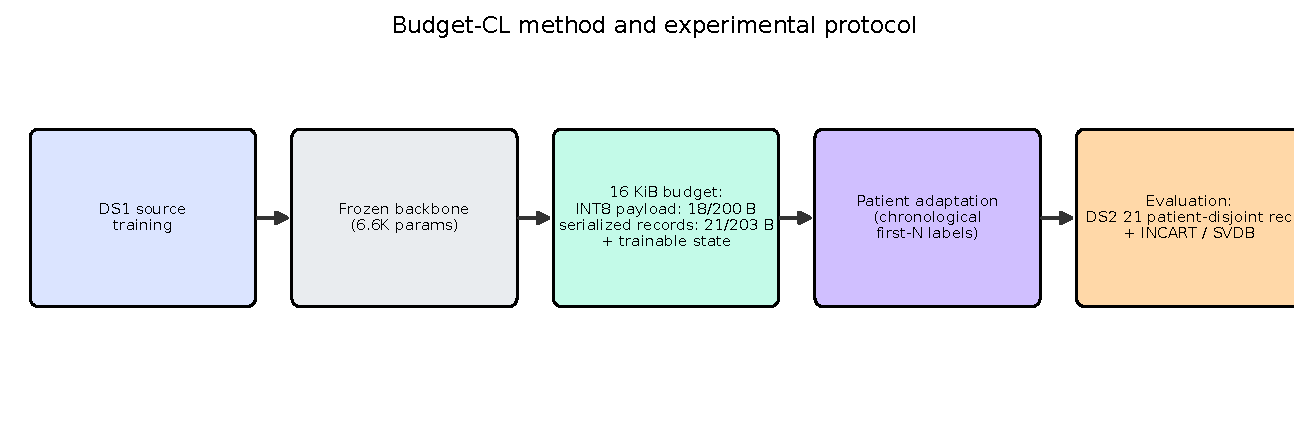
\includegraphics[width=\textwidth]{fig_method_protocol.pdf}
\caption{Method and experimental protocol. A DS1-trained tiny ECG transformer
is adapted per patient: source replay is mixed with the early (chronologically
first) labeled patient segment, while the later segment is held out for
testing: it contributes no beat, label, normalization statistic, early-stopping
signal, or model-selection information. The bounded whole-record filter
dependency near the chronological boundary is quantified and removed in the
split-first sensitivity analysis of Section~\ref{sec:splitfirst}. Adaptation may touch the classifier head, a post-pool residual
adapter, or an encoder-attention LoRA update, each drawing from the same
persistent-state budget. The budget covers persistent adaptation state; peak
temporary training memory and hardware runtime are not evaluated.}
\label{fig:protocol}
\end{figure}

\subsection{Analytical adaptation-state model}

\paragraph{What ``persistent state'' means here.} We use \emph{persistent
adaptation state} to mean \textbf{a statically reserved writable region that the
adaptation procedure needs across update steps}. It does \emph{not} imply that
every included quantity is nonvolatile or must survive power loss, and it is
\emph{not} total SRAM. The budget covers trainable weights, optimizer moments,
replay values, replay labels, and buffer metadata, all of which must persist
between updates. It also charges gradients, which are strictly update-time
working state rather than retained state; we include them because an
implementation that materializes a full gradient vector must reserve that region,
and excluding them would understate what a device has to set aside. It excludes
forward and backward activations, stack and workspace, and allocator overhead,
which are transient peak-SRAM quantities and are not measured anywhere in this
paper (Table~\ref{tab:memcats}).


A complete persistent-state accounting includes
\begin{equation}
B_{\mathrm{persistent}} =
B_{\mathrm{weights}}+B_{\mathrm{gradients}}+B_{\mathrm{optimizer}}
+B_{\mathrm{replay}}+B_{\mathrm{labels}}+B_{\mathrm{metadata}}+B_{\mathrm{padding}}.
\label{eq:completebudget}
\end{equation}
The experiments use FP32 trainable weights, FP32 gradients, and two FP32 Adam
moments, giving a per-parameter trainable cost of
\begin{equation}
b_{\mathrm{train}}=\underbrace{4}_{\text{weight}}+\underbrace{4}_{\text{grad}}
+\underbrace{8}_{\text{2 moments}}=16\ \mathrm{bytes/parameter}.
\end{equation}
A stored replay item costs more than the tensor it carries, and conflating the
two is an easy way to understate a budget. We therefore separate the
\emph{value payload} from the \emph{serialized record}:
\begin{equation}
b_l^{\mathrm{record}} =
b_l^{\mathrm{payload}} + b_{\mathrm{label}} + b_{\mathrm{flags}}
+ b_{\mathrm{pad}},
\label{eq:record}
\end{equation}
where $b_l^{\mathrm{payload}}$ is the INT8 tensor at replay location $l$ and the
remaining terms are the per-entry label, the validity and class-id flags, and any
alignment padding. Concretely
$b^{\mathrm{payload}} = 18\bytes \to b^{\mathrm{record}} = 21\bytes$ for
post-pool and $200\bytes \to 203\bytes$ for raw, at 1-byte alignment. For $P$
trainable parameters and $N$ replay items the reserved adaptation state is
\begin{equation}
B(P,N,l)=16P+N\,b_l^{\mathrm{record}}+B_{\mathrm{bufmeta}},
\label{eq:completebudget2}
\end{equation}
with $B_{\mathrm{bufmeta}}$ the fixed per-buffer overhead (write
index, count, reservoir state, class counters, and quantization parameters:
$49\bytes$ post-pool, $54\bytes$ raw). The constrained replay-count generator that
fixes a fair budget match is therefore
\begin{equation}
N_{\max}(P,l)=
\left\lfloor
\frac{B_{\mathrm{budget}}-16P-B_{\mathrm{bufmeta}}}
     {b_l^{\mathrm{record}}}
\right\rfloor .
\label{eq:nmax}
\end{equation}
Every byte total in this paper uses $b_l^{\mathrm{record}}$, never
$b_l^{\mathrm{payload}}$; where the text quotes 18 or 200 bytes it is naming the
payload explicitly.
Every configuration in this paper is generated from Eq.~\eqref{eq:nmax} so that
$B(P,N_{\max},l)\le 16{,}384\bytes$ holds by construction; the packed byte total
for each arm is asserted per adaptation cell. Table~\ref{tab:arm_definitions}
lists the resulting trainable counts, replay counts, and byte totals.

\paragraph{One-beat decision latency from the post-RR feature.} The model
consumes both the preceding and the \emph{following} RR interval. The following
interval is only known once the next R peak has been detected, so a classification
cannot be emitted at the current R peak: \textbf{the task evaluated here is
delayed heartbeat classification, one beat behind the signal}, not zero-latency
classification. This is a property of the source architecture we adopt rather
than of the adaptation method, and it applies equally to every arm including the
frozen baseline, so it does not affect any comparison in this paper. It does bound
the deployment claim, and comparing pre-RR-only, predicted-post-RR, and delayed
variants is left as future work.

\subsection{Replay-point cliff}

The base model accepts a 198-sample ECG window and two RR-derived interval
values. A convolutional embedding produces 66 tokens of width 16; the
feed-forward hidden dimension is 128; mean pooling then contracts the sequence,
and the two RR values are fused post-pool. Table~\ref{tab:replay_bytes} and
Fig.~\ref{fig:cliff} give the per-item INT8 payload at each candidate replay tap.
Only the post-pool (and post-pool$+$RR) representation is smaller than the raw
input; convolution tokens are $5.3\times$ and the FFN hidden tensor $42.7\times$
larger. The cliff is deterministic for this architecture and fixes \emph{where}
replay may be stored, but not \emph{where it should be}.

\begin{table}[H]
\centering
\small
\caption{Replay-point sizes and the \emph{serialized} INT8 cost of one stored
exemplar at each candidate tap. ``Values'' is the tensor itself; ``$+$RR'' adds
the two RR-interval features the model also consumes, without which an exemplar
cannot be replayed; ``$+$meta'' adds the per-entry label, valid flag, and class
id. The stride is the per-entry cost under 1-byte alignment, which is exact here
because every field is a byte. Only the post-pool tap is storage-compressive.}
\label{tab:replay_bytes}
\setlength{\tabcolsep}{5pt}
\begin{tabular}{llrrrrl}
\toprule
Replay point & Shape & Values & $+$RR & $+$meta & $\times$ raw & Verdict \\
\midrule
Raw ECG window          & $198\times1$  & 198   & 200   & 203   & $1.00$  & baseline \\
After conv embedding    & $66\times16$  & 1{,}056 & 1{,}058 & 1{,}061 & $5.33$  & larger (disqualified) \\
Encoder output          & $66\times16$  & 1{,}056 & 1{,}058 & 1{,}061 & $5.33$  & larger (disqualified) \\
FFN hidden              & $66\times128$ & 8{,}448 & 8{,}450 & 8{,}453 & $42.67$ & larger (disqualified) \\
Post-pool (mean)        & $16$          & 16    & 18    & 21    & $0.08$  & \textbf{smaller (viable)} \\
Post-pool $+$ RR concat & $18$          & 18    & 18    & 21    & $0.09$  & \textbf{smaller (viable)} \\
\bottomrule
\end{tabular}

\vspace{0.4em}
{\small Buffer-level fixed metadata is charged once, not per entry: a 4\,B write
index, a 4\,B count, 16\,B of reservoir state, $5\times4$\,B class counters, and a
4\,B scale plus 1\,B zero point per quantized tensor. That is 49\,B for a
post-pool buffer (one quantized tensor) and 54\,B for a raw buffer (two: the beat
and the RR pair). Under 4-byte alignment the strides become 24\,B and 204\,B;
we report the 1-byte figures and account for padding explicitly.}
\end{table}


\begin{figure}[H]
\centering
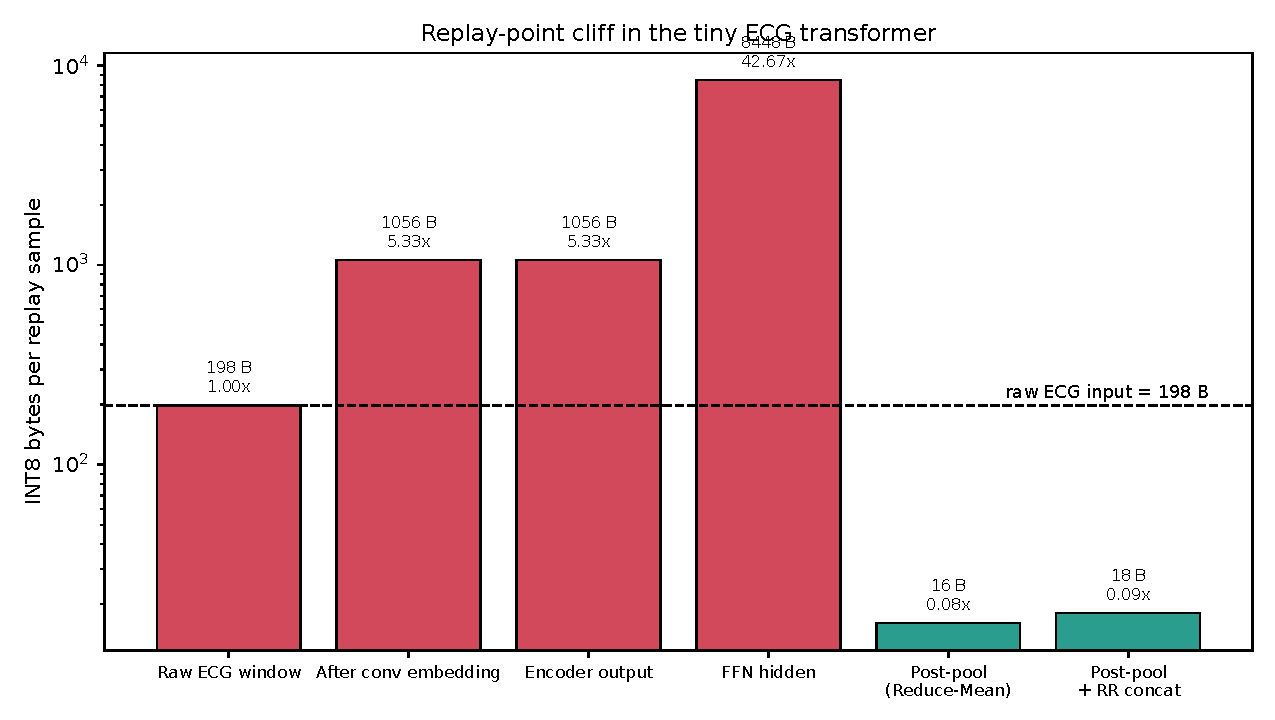
\includegraphics[width=0.82\textwidth]{fig_replay_cliff.pdf}
\caption{Replay-point cliff (log scale). Token and feed-forward representations
expand relative to the raw ECG window; only post-pool replay is
storage-compressive. Storing post-pool exemplars therefore maximizes replay
\emph{count}, which motivates---but does not justify---maximum-volume post-pool
replay.}
\label{fig:cliff}
\end{figure}

\subsection{Adaptation arms}

Six arms span the replay-volume / plasticity trade-off at 16\,KiB:
\begin{itemize}[leftmargin=*]
\item \textbf{A0} --- frozen source model (reference; 0 trainable, 0 replay);
\item \textbf{A1} --- 95-parameter linear head, maximum post-pool replay;
\item \textbf{A2} --- rank-1 post-pool residual adapter plus head, post-pool replay;
\item \textbf{A3} --- rank-2 post-pool residual adapter plus head, post-pool replay;
\item \textbf{A4} --- rank-1 encoder-attention LoRA plus head, raw replay;
\item \textbf{A5} --- rank-2 encoder-attention LoRA plus head, raw replay.
\end{itemize}
For fused representation $z\in\mathbb{R}^{18}$, the post-pool adapter applies
$z'=z+BAz$ with $A\in\mathbb{R}^{r\times18}$, $B\in\mathbb{R}^{18\times r}$. For
an encoder projection $W$, LoRA applies $W'=W+BA$ with
$A\in\mathbb{R}^{r\times d_{\mathrm{in}}}$, $B\in\mathbb{R}^{d_{\mathrm{out}}\times r}$.
A1--A3 spend the budget on \emph{volume}: 650--705 post-pool exemplars at
18\,B of payload each (21\,B serialized). A4--A5 spend it on \emph{depth}: only
52--62 raw exemplars at 200\,B payload (203\,B serialized) each, but expose the encoder to low-rank updates. For context,
full-model Adam-style trainable state would need $6643\times16=106{,}288$ bytes,
far beyond the ceiling, so full fine-tuning is infeasible under the constraint.
Fig.~\ref{fig:budget} shows how each arm partitions the same 16\,KiB.

\begin{table}[H]
\centering
\small
\caption{Complete arm definitions. ``Trainable tensors'' names exactly what
receives gradients; every other weight is frozen. Persistent bytes cover
trainable weights, gradients, two Adam moments per parameter, INT8 replay values,
per-entry label/valid/class-id metadata, buffer-level metadata, and alignment
padding. Replay counts are the maximum that fit, generated by the constrained
configuration generator. The right-hand block repeats the generation against an
effective ceiling of $15{,}360$\,B, i.e.\ a 1\,KiB firmware implementation
reserve; every arm was re-run at those reduced counts
(Section~\ref{sec:reserve}).}
\label{tab:arm_definitions}
\setlength{\tabcolsep}{4pt}
\begin{tabular}{llp{3.5cm}rrrrr}
\toprule
& & & & \multicolumn{2}{c}{16{,}384\,B ceiling} & \multicolumn{2}{c}{$+$1\,KiB reserve} \\
\cmidrule(lr){5-6}\cmidrule(lr){7-8}
Arm & Replay & Trainable tensors & Params & Items & Bytes & Items & Bytes \\
\midrule
A0 & ---       & none (frozen)                                   & 0   & 0   & 0        & 0   & 0 \\
A1 & post-pool & head $W,b$                                      & 95  & 705 & 16{,}374 & 656 & 15{,}345 \\
A2 & post-pool & post-pool adapter $B_1A_1$ $+$ head             & 131 & 678 & 16{,}383 & 629 & 15{,}354 \\
A3 & post-pool & post-pool adapter $B_2A_2$ $+$ head             & 167 & 650 & 16{,}371 & 601 & 15{,}342 \\
A4 & raw       & encoder LoRA $r{=}1$ on $W_{q,k,v,o}$ $+$ head  & 223 & 62  & 16{,}208 & 57  & 15{,}193 \\
A5 & raw       & encoder LoRA $r{=}2$ on $W_{q,k,v,o}$ $+$ head  & 351 & 52  & 16{,}226 & 47  & 15{,}211 \\
\midrule
R1 & ---       & encoder LoRA $r{=}1$ $+$ head, L2 source anchor & 223 & 0   & 3{,}568  & 0   & 3{,}568 \\
R2 & raw       & encoder LoRA $r{=}1$ $+$ head, L2 source anchor & 223 & 62  & 16{,}208 & 57  & 15{,}193 \\
\bottomrule
\end{tabular}

\vspace{0.4em}
{\small All arms use Adam ($b_{\mathrm{train}} = 16$\,B/parameter: 4 weight,
4 gradient, 8 for two moments), FP32 weights, and INT8 replay. Replay and target
beats are concatenated rather than mixed at a fixed per-batch ratio, so the
effective replay fraction is $N_{\mathrm{replay}}/(N_{\mathrm{replay}} +
N_{\mathrm{target}})$ with $N_{\mathrm{target}} = 500$. The R-arm source anchor
adds \emph{no} persistent bytes: the anchor is the frozen base weight, which is
already stored for inference.}
\end{table}


\begin{figure}[H]
\centering
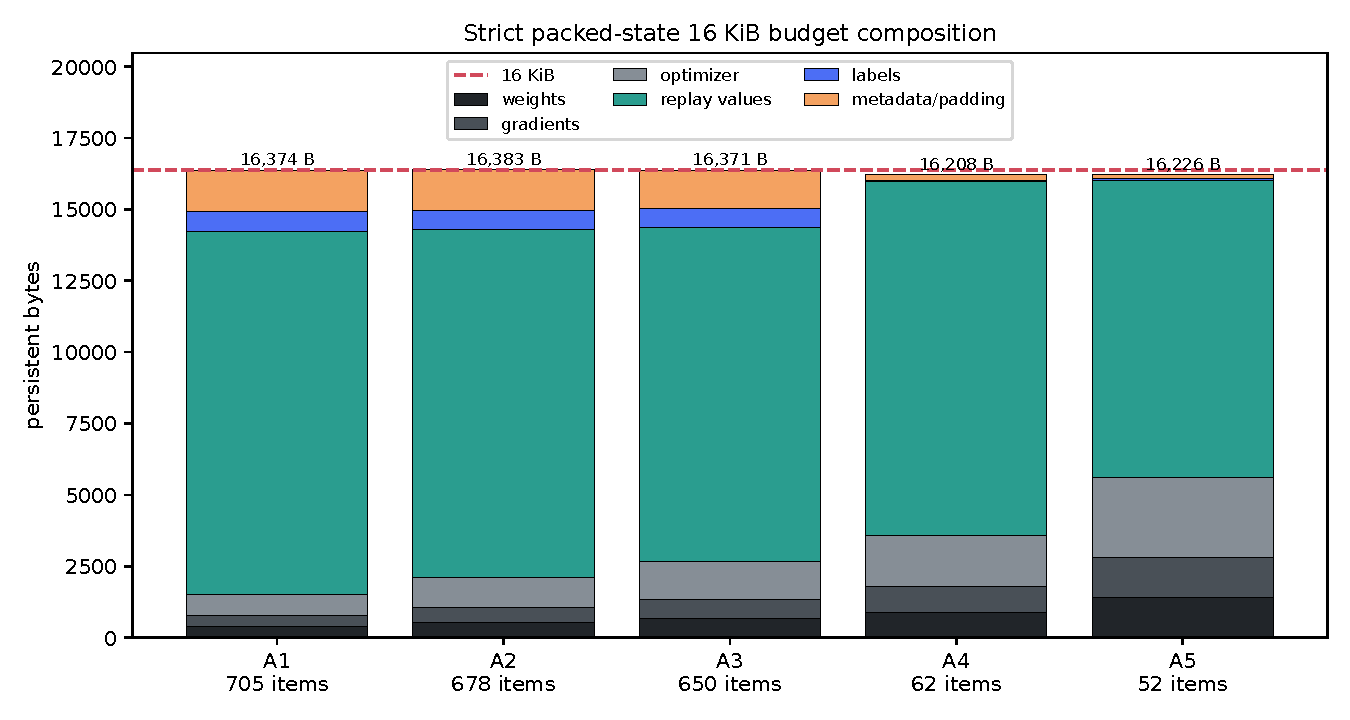
\includegraphics[width=0.80\textwidth]{fig_budget_composition.pdf}
\caption{Persistent-state composition of each arm at 16\,KiB. Volume arms
(A1--A3) allocate almost the entire budget to replay values; depth arms
(A4--A5) shift bytes into trainable weights, gradients, and optimizer moments,
leaving room for only tens of raw exemplars.}
\label{fig:budget}
\end{figure}

\section{Experimental Protocol}
\label{sec:protocol}

\subsection{Source data and source training}

The source backbone is trained \emph{only} on the de Chazal DS1 partition of the
MIT--BIH Arrhythmia Database. As published, DS1 and DS2 are \emph{record}-disjoint
rather than patient-disjoint (Section~\ref{sec:cohort}); the cohort correction
below is what makes the evaluation set genuinely patient-disjoint from DS1. The
model has 6{,}643
parameters and the architecture dimensions of Section~\ref{sec:method}. DS2
records never enter source training. On the held-out DS1 test split the frozen
source attains \macrof{} $=0.749$ over all five AAMI classes and $0.946$ over
the supported N/S/V classes, with strong V sensitivity but comparatively weak S
behavior---the regime in which patient-specific adaptation is expected to help.

\subsection{Primary and secondary cohorts}
\label{sec:cohort}

\paragraph{The de Chazal split is not patient-disjoint, and we correct it.} The
DS1/DS2 partition is the standard inter-patient protocol and we adopt it, but it
contains one subject that appears on both sides. MIT--BIH record 202's own WFDB
header states that it ``was taken from the same analog tape as record 201''
\cite{mitdb202note}, and
the two records carry identical demographics (68\,M, identical medication list).
Record \textbf{201 is in DS1} and record \textbf{202 is in DS2}. A source model
trained on DS1 has therefore already seen this subject, and evaluating adaptation
on record 202 as though it were an unseen patient measures partly memorization
rather than personalization.

We audited all 48 MIT--BIH records for this failure mode, comparing header
demographics and explicit same-tape annotations, and found exactly one such
cross-split pair: 201/202. \textbf{We exclude record 202 from the evaluation
cohort}, leaving \textbf{21 genuinely patient-disjoint records}. The source model
is unchanged, since 201 remains a legitimate DS1 training record; only the
evaluation set changes. Every primary and corrected analysis uses the 21-record
cohort. One explicitly labelled historical sensitivity result retains the earlier
22-record split and is not compared with the primary results
(Section~\ref{sec:lowbyte}). The primary grid is
$6\ \text{arms}\times21\ \text{records}\times5\ \text{seeds}=630$ adaptation
cells. We flag this because the contaminated 22-record version is what a
straightforward reading of the de Chazal protocol produces, and results computed
that way are not strictly patient-disjoint and may be optimistically biased ---
on our own data, removing record 202
raised every arm mean slightly but cost the A4--A3 comparison its statistical
significance.

\textbf{Primary cohort.} The 21 patient-disjoint DS2 records after the
\emph{post hoc} subject-identity correction form the primary cohort. Records are \emph{not}
selected using test-segment arrhythmia burden. This removes the selection bias of
the earlier exploratory panel and is the cohort behind every headline result.
Table~\ref{tab:dataset_manifest} lists the record IDs, seeds, class supports, and
split rule.

\textbf{Secondary cohort.} The 12-record arrhythmia-informative panel (records
whose test window contains $\ge 30$ arrhythmic beats) is retained only as
secondary evidence for class-specific behavior, and is clearly labeled as such
wherever it appears.

\begin{table}[H]
\centering
\small
\caption{Dataset, split, and preprocessing manifest for every database used.
MIT--BIH records are one per subject \emph{after} removing record 202, which
shares a subject with DS1 record 201 and would otherwise break patient
disjointness (Section~\ref{sec:cohort}). INCART contains multiple recordings per
subject, so its statistical unit is the subject; the full per-record inclusion
and exclusion manifests are released with the code.
\textbf{The eligibility rules are not symmetric, and the difference matters:}
primary MIT--BIH inclusion is \emph{outcome-blind} --- every corrected DS2
record is used and test-segment arrhythmia burden plays no part --- whereas the
external subsets additionally require $\ge 30$ S$+$V beats \emph{in the test
window}, so external eligibility uses future test labels and enriches those
cohorts for recordings where minority-class adaptation can be evaluated at
all.}
\label{tab:dataset_manifest}
\setlength{\tabcolsep}{5pt}
\begin{tabular}{llll}
\toprule
Field & MIT--BIH (primary) & INCART & SVDB \\
\midrule
Role & source (DS1) $+$ target (DS2) & external target & external target \\
Records evaluated & \textbf{21} (DS2) & 11 & 46 \\
Unique subjects & \textbf{21} & \textbf{6} & 46 \\
Records available & 48 & 75 & 78 \\
Lead & MLII & II & ECG1 \\
Native sampling rate & 360\,Hz & 257\,Hz & 128\,Hz \\
Resampling & none & \multicolumn{2}{l}{\texttt{resample\_poly} to 360\,Hz} \\
Beat window & \multicolumn{3}{l}{198 samples, R-peak centred (99 left / 99 right)} \\
R-peak source & \multicolumn{3}{l}{WFDB \texttt{atr} annotations} \\
Filtering & \multicolumn{3}{l}{baseline-wander removal $+$ low-pass} \\
RR normalization & \multicolumn{3}{l}{MIT--BIH DS1 statistics only, clipped at $\pm2$} \\
AAMI mapping & \multicolumn{3}{l}{N / S / V / F / Q; non-beat symbols ignored} \\
Adaptation protocol & \multicolumn{3}{l}{chronological first 500 labels, $\mathrm{gap\_beats}=1$, rest test} \\
Eligibility rule & \textbf{all corrected DS2;} & $\ge 30$ S$+$V beats & $\ge 30$ S$+$V beats \\
 & \textbf{no test-burden filter} & in the test window & in the test window \\
Eligibility uses test labels? & \textbf{no} (outcome-blind) & \textbf{yes} & \textbf{yes} \\
Seeds & \multicolumn{3}{l}{$\{42,43,44,45,46\}$} \\
\midrule
DS1 records & \multicolumn{3}{p{9.2cm}}{101 106 108 109 112 114 115 116 118 119 122 124 201 203 205 207 208 209 215 220 223 230} \\
DS2 records & \multicolumn{3}{p{9.2cm}}{100 103 105 111 113 117 121 123 200 210 212 213 214 219 221 222 228 231 232 233 234 \quad(\emph{202 excluded: same subject as DS1 record 201})} \\
\bottomrule
\end{tabular}
\end{table}


\subsection{Chronological adaptation}

Each record is split in annotation (temporal) order. The chronologically first
labeled beats form the adaptation set; a single unlabeled guard beat
($\mathrm{gap\_beats}=1$) is dropped to prevent centered-window overlap between
adaptation and test; all later beats are test-only. Early stopping uses only a
slice of the adaptation union and never the test segment. Streamed patient beats
are not counted as persistent replay storage---only the fixed source replay
memory $\mathcal{R}_0$ is. Every patient resets to $\theta_0$. The primary
run therefore contains $6\ \text{arms}\times21\ \text{records}\times5\
\text{seeds}=630$ adaptation cells (seeds $\{42,43,44,45,46\}$).

\subsection{Signal preprocessing, stated exactly}
\label{sec:preproc}

Every record passes through the same front end before beat extraction, applied to
the whole signal rather than per window. The pipeline is inherited unchanged from
the source architecture we adopt \cite{busia2025tiny}, so that our adaptation
results are attributable to the adaptation method rather than to a different
front end.
\textbf{Baseline-wander removal} uses two cascaded median filters: a 200\,ms
kernel strips the QRS and P complexes leaving baseline plus T-wave, a 600\,ms
kernel on that result strips the T-wave, and the remaining baseline estimate is
subtracted from the original signal. Kernel lengths are rounded to the nearest
odd sample count at the record's own sampling rate.
\textbf{Noise suppression} is a 4th-order Butterworth low-pass at 35\,Hz applied
\emph{zero-phase} (forward--backward, \texttt{filtfilt}), which is
non-causal: it uses future samples and could not run unmodified in a streaming
device. We keep it because it matches the source model's published front end, and
we flag it as a deployment gap rather than a result.
\textbf{Resampling} to 360\,Hz uses polyphase resampling
(\texttt{resample\_poly}) and is applied to external databases only (INCART
257\,Hz, SVDB 128\,Hz); MIT--BIH is already at 360\,Hz.

\paragraph{Non-causal preprocessing crosses the chronological boundary.} All
three of those operations --- both median kernels and the zero-phase low-pass ---
are applied to the \emph{whole record} before the chronological split, and all
three are non-causal. An adaptation-side sample within the filters' backward
reach of the split therefore depends on raw samples that belong to the test
segment. Test \emph{labels} are never involved, and no test beat enters
adaptation, but the test \emph{signal} is not strictly unseen, so the released
protocol is properly described as \textbf{offline chronological label
partitioning with non-causal whole-record preprocessing} rather than as strictly
causal chronological adaptation.

We bounded the reach empirically rather than assuming it: injecting a truncation
at a boundary and measuring how far the difference propagates backwards gives a
one-sided influence of $84$ samples at a $10^{-3}$ relative tolerance and
$120$ samples ($333$\,ms) at $10^{-5}$ --- shorter than a single RR interval.
Because a beat window spans $198$ samples, only the last one or two adaptation
beats of a record can be affected at all. Section~\ref{sec:splitfirst} reports a
split-first rerun that removes the dependency entirely and quantifies what it
changes.
\textbf{Beat windows} are 198 samples centred on the annotated R peak, 99 left
and 99 right; windows that would extend past a record boundary are dropped rather
than padded. \textbf{R peaks} come from the WFDB \texttt{atr} annotations, never
from a detector, so detector error is excluded from this study by construction.
\textbf{Labels} follow the AAMI N/S/V/F/Q mapping; non-beat annotation symbols
and symbols outside the mapping are skipped.
\textbf{RR features} are the preceding and following intervals in seconds,
normalized with MIT--BIH DS1 statistics only ($\mu = 0.7785$\,s,
$\sigma = 0.4956$\,s) and clipped to $\pm 2$; no target-database statistic ever
enters normalization.

\subsection{Replay quantization, stated exactly}
\label{sec:quant}

Replay values are stored INT8 with \textbf{symmetric, per-tensor} quantization.
For a stored tensor $x$ the buffer holds
\begin{equation}
q=\operatorname{clip}\!\left(\operatorname{round}\!\left(x/s\right),-127,127\right),
\qquad
\hat{x}=s\,q,
\qquad
s=\frac{\max|x|}{127},
\label{eq:quant}
\end{equation}
where the scale $s$ is calibrated by absolute maximum over the whole buffer at
the moment it is written, and the zero point is fixed at $0$ by symmetry. One
FP32 scale is stored per quantized tensor: one for a post-pool buffer, and two
for a raw buffer, which quantizes the beat and the RR pair on separate scales.
Per-row scales are deliberately \emph{not} used, because a scale per exemplar
would add 4\,B per entry and is already charged as buffer metadata in
Eq.~\eqref{eq:completebudget2}. During adaptation the buffer is dequantized back
to FP32 by Eq.~\eqref{eq:quant} before entering the graph, so training sees
exactly the INT8-rounded values a device would replay --- the quantization error
is inside the experiment, not idealized away.

\subsection{Replay-buffer construction}
\label{sec:replay_policy}

The replay policy is held fixed across every arm so that the comparison isolates
allocation rather than selection quality. The buffer is drawn once from the DS1
source pool by a \textbf{maximum-volume class-balanced selector}: each of the
five AAMI classes receives an equal quota $\lfloor N/5 \rfloor$, and because rare
classes exhaust their pool before the quota is met, the unfilled slots are
redistributed round-robin among classes that still have examples rather than
being wasted. The selector is seeded by the run seed, so the buffer is
\emph{fixed across patients} within a seed and \emph{resampled across seeds};
patient-to-patient variation therefore cannot come from a changing buffer, while
seed-to-seed variation includes buffer variation, which is the conservative
choice.

Values are stored INT8 with a per-tensor scale and zero point. A raw entry stores
the ECG window \emph{and} its RR pair, since the model consumes both and a window
alone cannot be replayed; the honest per-item cost is therefore 200\,B of values
rather than the 198\,B of the window alone, and the budget assertion uses 200.
Post-pool entries are extracted once from the frozen source encoder and are
therefore \emph{stale by construction}: they are never re-extracted as adaptation
proceeds, which is exactly why a post-pool buffer cannot track a representation
that is itself changing --- and is one reason a post-pool buffer pairs naturally
with a frozen encoder. Raw entries carry no such staleness because they are
re-forwarded through the current model on every update, at a greater but
unmeasured compute cost (Appendix~\ref{sec:embedded}). Replay and target beats are
concatenated into one training set rather than mixed at a fixed per-batch ratio,
so the effective replay ratio is $N_{\mathrm{replay}} / (N_{\mathrm{replay}} +
N_{\mathrm{target}})$. There is no eviction policy: the buffer is written once
and never replaced, since the source distribution is static.

\subsection{Metrics and statistical analysis plan}

\paragraph{The primary metric, stated exactly.} For patient $p$ let $n_{p,c}$ be
the number of test beats of AAMI class $c$. The scored class set and the primary
metric are
\begin{equation}
\mathcal{C}_p = \{c \in \{\mathrm{N},\mathrm{S},\mathrm{V}\} : n_{p,c} \ge n_{\min}\},
\qquad
F1_{\mathrm{macro},p} = \frac{1}{|\mathcal{C}_p|}\sum_{c \in \mathcal{C}_p} F1_{p,c},
\label{eq:metric}
\end{equation}
with $n_{\min} = 1$: a class counts as present if the patient's test segment
contains at least one beat of it. The remaining conventions are fixed as follows.
The class set is N/S/V. Fusion (F) is excluded from the primary metric because it
is absent from most DS2 test segments, so including it would make the
denominator $|\mathcal{C}_p|$ vary for reasons unrelated to performance; F is
reported separately as a pooled secondary metric, where the encoder arms show
their largest relative gain. The unclassifiable class Q is excluded because the
source model is not trained to separate paced and unclassifiable beats and the
protocol makes no claim about them. A class with $n_{p,c} = 0$ is omitted from
the average rather than scored as zero, since scoring an absent class as zero
would penalize a patient for the composition of their own record. Precision and
recall use the zero-division convention $0/0 = 0$, which applies only when a
present class receives no predictions.

Secondary metrics are pooled accuracy, per-class S/V/F sensitivity, precision,
and F1, the fraction of patients improved versus A0, and source-domain \macrof{}
change $\Delta^{\mathrm{src}}$ (Eq.~\ref{eq:gain_and_srcchange}), which is negative when
adaptation costs source performance. Pooled and per-patient summaries are both reported because a
single record (232) contributes a large fraction of the pooled S beats, so pooled
scores alone would be misleading. Because the improved-patient count is sensitive
to how small changes are treated, we report it both threshold-free and at a
meaningful-change threshold of $0.02$ \macrof{} (Table~\ref{tab:harm}).

The primary metric, seed count, paired tests, effect-size definition, and Holm
comparison family were fixed before the final runs. Record 202 was excluded after
a subject-identity audit showed that it belongs to the same patient as DS1
record 201 (Section~\ref{sec:cohort}); all affected analyses were rerun without
changing the methods or the comparison family.

Seeds are averaged per patient before
patient-wise paired tests. For each planned comparison we report the mean and
median paired difference, a \textbf{patient bootstrap} 95\% confidence
interval ($10{,}000$ resamples), a paired Wilcoxon signed-rank $p$-value,
rank-biserial effect size, and a Holm correction across the six-comparison
family $\{$A4--A1, A5--A1, A4--A2, A4--A3, A4--A0, A5--A0$\}$. A leakage and
reproducibility audit (no DS1/DS2 record overlap, no adaptation/test window
crossing, no \emph{primary-cohort} test label used for patient inclusion,
replay selection, early stopping, hyperparameter selection, or adaptation ---
external inclusion and the class-aware oracle deliberately do use test-window
labels and are excluded from this check (Sections~\ref{sec:rq6}
and~\ref{sec:rq7}) --- source-only
normalization statistics, stored seeds and library versions, recorded source
checkpoint hash) accompanies the run and returns PASS\,11 / FIXED\,1 / ASSESSED\,1 / WARN\,1 /
FAIL\,0.

\paragraph{The bootstrap, stated exactly.} Every interval in this paper is a
\emph{patient bootstrap}, and we name it that way consistently because seeds are
collapsed before resampling: (i) average the five seeds within each patient to
give one score per patient; (ii) resample the 21 patients with replacement;
(iii) recompute the arm mean or the paired difference on the resampled patients;
(iv) repeat $10{,}000$ times and take the $2.5$th and $97.5$th percentiles.
Seeds are therefore not resampled, and we \textbf{do not} call this a
hierarchical bootstrap --- that term is reserved for a procedure that resamples
seeds inside every resampled patient, which would be the right choice if
seed variance were the quantity of interest. External-database intervals use the
same procedure with subjects in place of patients.

\section{Results}
\label{sec:results}

We organize the evidence around seven research questions.
\textbf{RQ1:} where is replay memory-compressing? \textbf{RQ2:} does encoder
plasticity improve patient adaptation? \textbf{RQ3:} is the gain caused by
replay, plasticity, or both? \textbf{RQ4:} is the 16\,KiB operating point itself
a limitation? \textbf{RQ5:} does the result survive a class-reweighted
source model? \textbf{RQ6:} does it transfer across databases? \textbf{RQ7:} how
many labels are required?

\paragraph{Which results are pre-specified.} RQ1--RQ3 and the source-domain
change analysis follow a pre-specified plan: the primary metric (per-patient
\macrof{} over present N/S/V classes), the unit of analysis (patient), the
all-DS2 cohort, the seed count, the paired test, the effect size, and the
six-comparison Holm family were all fixed in a written analysis plan before the
final runs, and the six comparisons reported in Table~\ref{tab:pairwise_tests}
are exactly that pre-specified family with no additions. \textbf{One departure
from a strict reading of ``pre-specified'' must be stated:} record 202 was
excluded \emph{after} the subject-identity audit described in
Section~\ref{sec:protocol}, and every affected analysis was rerun. The exclusion
changed the cohort, not the methods --- no metric, test, effect size, or
comparison family was altered in response to seeing results. RQ4--RQ7 are \textbf{secondary and exploratory}: they were specified
after the primary analysis, they use reduced panels or different cohorts, and
their $p$-values are not part of the corrected family. We flag the cohort and
seed count at the head of each secondary subsection because they differ.

\subsection{RQ1 --- The replay-point cliff}

\textbf{Takeaway:} only the post-pool representation is storage-compressive;
every intermediate tap is several times larger than the raw beat, so the
architecture fixes \emph{where} replay can be cheap.

The cliff is a deterministic property of the architecture
(Table~\ref{tab:replay_bytes}, Fig.~\ref{fig:cliff}). A raw beat costs 198\,B,
the convolution/encoder tokens $1{,}056$\,B ($5.3\times$), the FFN hidden tensor
$8{,}448$\,B ($42.7\times$), and only the post-pool$+$RR vector is smaller at
18\,B ($0.09\times$). Consequently, the frozen source model can afford 705
post-pool exemplars but only 62 raw exemplars in the same 16\,KiB
(Table~\ref{tab:arm_definitions}). RQ1 confirms that the cliff constrains
\emph{where} replay is cheap; the remaining questions ask whether cheap replay
is the best use of the budget.

\subsection{RQ2 --- Patient-level adaptation gain}

\textbf{Takeaway:} both encoder-LoRA arms beat the frozen model with a large
effect (significant after Holm correction under the pre-registered primary test;
Table~\ref{tab:pairwise_tests}) and improve 16 of 21 patients, against 12 of 21
for maximum head-only replay, with stronger pooled minority-class performance.

Table~\ref{tab:primary_arms} reports the all-DS2 primary result: per-patient
\macrof{} (seeds median-aggregated within patient, the pre-registered locked
estimator), the number of patients improved versus A0, and pooled S-class F1.
Both encoder-LoRA arms dominate the frozen model and improve the most patients.
A5 reaches the best per-patient score ($0.811\pm0.179$) and A4 nearly matches it
($0.810\pm0.176$) at the same 16/21 improved count; by contrast,
maximum-volume head-only replay (A1) improves only 12/21 patients despite storing
$\approx 11\times$ more exemplars. Fig.~\ref{fig:primary} shows
the per-patient distribution and Fig.~\ref{fig:waterfall} the sorted per-patient
gain; both make clear that the mean is carried by a minority of patients.

\paragraph{Seed stability.} A descriptive point that costs nothing and does not
depend on the inconclusive superiority comparison: the arms differ sharply in how
much their arm-level score depends on the seed-aggregation rule. Comparing
mean-over-seeds and median-over-seeds central values
(\texttt{results/r0\_estimator\_matrix.csv}), maximum head-only replay (A1) moves
$0.786 \to 0.743$, a $0.043$ gap---its arm mean sits well above its median because
a minority of favourable seeds inflate it---while rank-1 LoRA (A4) moves
$0.803 \to 0.777$ ($0.026$) and rank-2 LoRA (A5) is essentially
aggregation-invariant at $0.809$ versus $0.813$ ($0.004$). Maximum head-only
replay is thus the \emph{least seed-stable} arm tested and the proposed encoder
arms the most stable. No test was pre-registered for this contrast, so we report
it descriptively.
Aggregate means hide the fact that adaptation is not uniformly beneficial, so we
report the harm side explicitly, and we report it at two thresholds because the
choice of threshold changes the story materially.

Counting any decline as harm, the encoder arms harm two (A4) and three (A5) of 21
patients and maximum head-only replay harms 8, which makes the encoder arms look
safer. That impression does not survive a meaningful threshold. Defining the harm
rate $R_{\mathrm{harm}} = |\{p : G_p < -\epsilon\}| / P$ with $\epsilon = 0.02$
stated before analysis, the counts become A1 $0/21$
($R_{\mathrm{harm}} = 0.000$), A2 $2/21$, A3 $3/21$, A4 $2/21$, and A5 $2/21$
(Table~\ref{tab:harm}) --- so on this measure \textbf{maximum head-only replay is
the \emph{safest} arm}, harming nobody measurably, while the encoder arms each
harm two patients. \textbf{Most of the apparent harm
advantage of the encoder arms is sub-threshold noise}: at $\epsilon = 0.02$ the
adapted arms harm zero (A1) to three (A3) patients each. The same correction
applies to the improvement counts: the headline 16/21 for A4 and A5 falls to
12/21 when small changes are excluded, against 10/21 for A1. The encoder arms
remain ahead on the improvement count, but by two patients rather than four, and
they are \emph{worse} on the harm count. What separates them is the size of the
tail loss rather than its frequency: A4's worst patient loses $0.029$ where A3's
loses $0.050$ and A5's $0.112$.

We keep the threshold-free counts in Table~\ref{tab:primary_arms} because they
are what the pre-specified plan defined, and report the thresholded counts beside
them so that neither is read alone. Either way the practical conclusion is the
same: personalization helps most patients, measurably harms a few, and a
deployment would need a per-patient acceptance check --- adapt, evaluate on
held-out adaptation-side data, and fall back to the frozen model if the gain is
not positive --- rather than an assumption that adaptation always helps.

\begin{table}[H]
\centering
\small
\caption{Patient-harm profile on the 21-record patient-disjoint cohort, seeds
averaged. $G_p$ is the per-patient change in the primary metric against the
frozen model A0. Improved / unchanged / harmed use a meaningful-change threshold
$\epsilon = 0.02$ stated before analysis, and
$R_{\mathrm{harm}} = |\{p : G_p < -\epsilon\}| / P$. ``Impr.\ ($>0$)'' repeats
the threshold-free count from Table~\ref{tab:primary_arms}.}
\label{tab:harm}
\setlength{\tabcolsep}{4pt}
\begin{tabular}{lrrrrrrrrrr}
\toprule
Arm & Mean $G_p$ & Med.\ $G_p$ & Impr. & Unch. & Harmed & $R_{\mathrm{harm}}$ & Min $G_p$ & 5th pct. & Max $G_p$ & Impr.\ ($>0$) \\
\midrule
A1 & $+0.119$ & $+0.028$ & 11 & 10 & \textbf{0} & \textbf{0.000} & $-0.017$ & $-0.016$ & $+0.793$ & 12 \\
A2 & $+0.124$ & $+0.040$ & 12 & 8  & 1 & 0.048 & $-0.069$ & $-0.020$ & $+0.789$ & 15 \\
A3 & $+0.109$ & $+0.037$ & 11 & 8  & 2 & 0.095 & $-0.052$ & $-0.036$ & $+0.770$ & 13 \\
A4 & $+0.136$ & $+0.035$ & \textbf{12} & 7 & 2 & 0.095 & $\mathbf{-0.034}$ & $-0.027$ & $+0.804$ & \textbf{17} \\
A5 & $+0.143$ & $+0.037$ & \textbf{12} & 7 & 2 & 0.095 & $-0.123$ & $-0.024$ & $+0.804$ & \textbf{17} \\
\bottomrule
\end{tabular}
\end{table}


% GENERATED FILE -- do not edit by hand.
% Regenerate with: python3 scripts/r1_regen_primary_tables.py
\begin{table}[H]
\centering
\small
\caption{Per-patient \macrof{} over the 21-record patient-disjoint cohort, five seeds \textbf{median-aggregated within patient} (the pre-registered locked estimator). Intervals are patient bootstraps ($10{,}000$ resamples).}
\label{tab:primary_arms}
\begin{tabular}{lrrrl}
\toprule
Arm & Mean & SD & Median & 95\% CI \\
\midrule
A0 (frozen) & $0.666$ & $0.245$ & $0.666$ & $[0.563, 0.766]$ \\
A1 (head $+$ max replay) & $0.785$ & $0.177$ & $0.743$ & $[0.712, 0.859]$ \\
A2 (post-pool $r{=}1$) & $0.792$ & $0.179$ & $0.763$ & $[0.717, 0.866]$ \\
A3 (post-pool $r{=}2$) & $0.767$ & $0.180$ & $0.739$ & $[0.693, 0.844]$ \\
A4 (LoRA $r{=}1$) & $0.810$ & $0.176$ & $0.777$ & $[0.737, 0.884]$ \\
A5 (LoRA $r{=}2$) & $0.811$ & $0.179$ & $0.813$ & $[0.737, 0.886]$ \\
\bottomrule
\end{tabular}
\end{table}


\begin{figure}[H]
\centering

\includegraphics[width=0.92\textwidth]{fig_patient_distribution.pdf}
\caption{Per-patient \macrof{} across the 21-record primary cohort (five seeds
averaged within patient, so each point is one patient). Boxes show the median
and interquartile range; grey lines follow a single patient across arms. The
encoder-LoRA arms (A4, A5) shift the distribution upward, but the spread is
wide and heavily patient-dependent: the mean gain is not evenly distributed.}
\label{fig:primary}
\end{figure}

\begin{figure}[H]
\centering
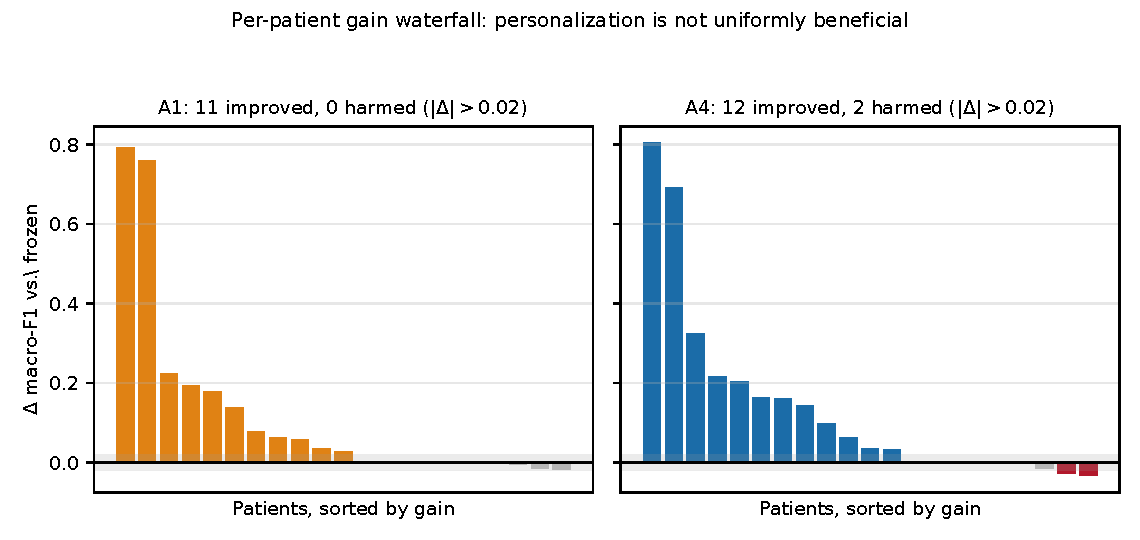
\includegraphics[width=0.95\textwidth]{fig_patient_waterfall.pdf}
\caption{Per-patient gain against the frozen model, sorted, for maximum
head-only replay (A1) and rank-1 encoder LoRA (A4) on the primary cohort. The
grey band is the meaningful-change threshold $|\Delta| \le 0.02$ \macrof{};
bars inside it are indistinguishable from no change, and red bars are harmed
patients. A small number of patients contribute most of the mean gain. At
$\epsilon = 0.02$ the encoder arm (A4) harms two patients while maximum
head-only replay (A1) harms none.}
\label{fig:waterfall}
\end{figure}

Pooled beat-level behavior tells the same story on minority classes
(Table~\ref{tab:pooled}, Fig.~\ref{fig:class}). The frozen model labels the
overwhelming majority of pooled S beats as normal (S F1 $=0.145$); every
adaptation arm recovers S, but the encoder arms are strongest, reaching S F1
$0.832$--$0.835$ and lifting fusion (F) F1 from $0.000$ to $0.578$--$0.604$ where
the post-pool arms stall near $0.39$. Pooled accuracy rises from $0.873$ (A0) to
$0.974$ (A5).

\begin{table}[H]
\centering
\small
\caption{Pooled beat-level performance over the 21-record primary cohort
($32{,}768$\,N / $1{,}385$\,S / $2{,}564$\,V / $291$\,F test beats). Each
record contributes its seed-mean confusion matrix, so the supports are test
beats rather than seed-multiplied decisions. Best in each column in bold.}
\label{tab:pooled}
\begin{tabular}{lrrrr}
\toprule
Arm & Pooled acc. & S F1 & V F1 & F F1 \\
\midrule
A0 & 0.873 & 0.145 & 0.728 & 0.000 \\
A1 & 0.962 & 0.776 & 0.915 & 0.416 \\
A2 & 0.960 & 0.786 & 0.904 & 0.395 \\
A3 & 0.960 & 0.773 & 0.909 & 0.392 \\
A4 & 0.973 & 0.832 & 0.934 & 0.578 \\
A5 & \textbf{0.974} & \textbf{0.835} & \textbf{0.938} & \textbf{0.604} \\
\bottomrule
\end{tabular}
\end{table}

\begin{figure}[H]
\centering
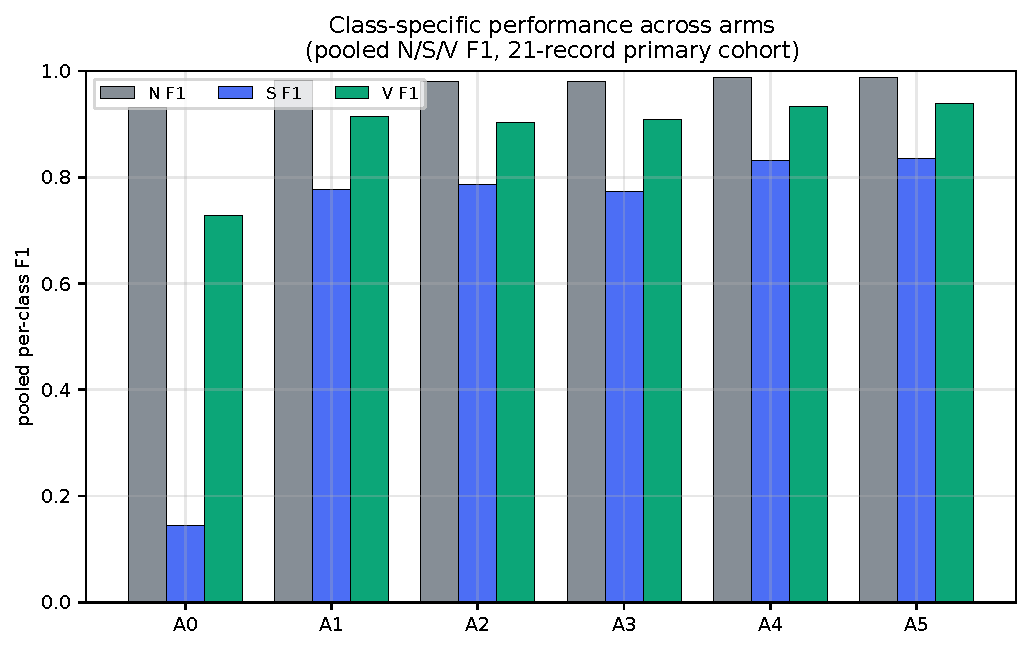
\includegraphics[width=0.90\textwidth]{fig_class_specific.pdf}
\caption{Class-specific pooled performance with the frozen baseline. Adaptation
concentrates its benefit on the minority S class while preserving N and V;
encoder arms give the largest minority-class gains. The fusion (F) class is not
shown here because it is absent from most patients' test segments; pooled F1
for F is reported in Table~\ref{tab:pooled}, where the encoder arms show their
largest relative improvement ($0.000 \to 0.58$--$0.60$ against $\approx 0.39$
for the post-pool arms).}
\label{fig:class}
\end{figure}

\paragraph{Direct paired tests.} Table~\ref{tab:pairwise_tests} and
Fig.~\ref{fig:forest} report the six pre-registered comparisons under the primary
median-seed aggregation, with Holm correction, superiority, and the
pre-registered equivalence test ($\delta = 0.02$ \macrof{}, 90\% BCa interval of
the median paired difference; Section~\ref{sec:protocol}). Both encoder arms
significantly beat the frozen model: A4--A0 median $+0.040$ (95\% BCa CI
$[0.000,0.137]$, Holm $p=0.007$, rank-biserial $0.91$) and A5--A0 median $+0.038$
(CI $[0.000,0.140]$, Holm $p=0.017$, rank-biserial $0.81$). \textbf{These are the
only two comparisons that survive Holm correction.} The \emph{direct} comparisons
against maximum head-only replay are \emph{inconclusive}, not null: A4--A1 has a
median difference of $+0.0007$ and A5--A1 of $+0.0034$ (both Holm $p=0.079$), yet
their 90\% equivalence intervals ($[0.000,0.024]$ and $[0.000,0.029]$) are not
contained in $[-0.02,+0.02]$, so equivalence within the pre-specified margin is
\emph{not} declared either. This 21-patient design detects a median shift no
smaller than its minimum detectable effect ($\approx 0.010$--$0.040$ \macrof{}
across the family; Table~\ref{tab:pairwise_tests}), and the observed A4--A1
median lies below it. The one head-only contrast that \emph{does} clear the
equivalence test is A4 versus the rank-1-equivalent post-pool adapter A2 (90\% CI
$[0.000,0.016] \subset [-0.02,+0.02]$). The honest reading is a bounded
replay--plasticity \emph{allocation} frontier: encoder plasticity reaches
significance against the frozen baseline where post-pool volume does not and
improves more patients (16/21 vs 12/21), while its direct superiority over
maximum replay is neither established nor excluded at this sample size---not
``depth beats volume.'' \textbf{The A4--A1 equivalence verdict is not robust and
turns on a single record.} With all 21 records the $90\%$ BCa upper bound is
$0.0240$, above the $\delta = 0.020$ margin, so equivalence is \emph{not}
declared; dropping record 232 alone lowers that bound to $0.0198$---below the
margin by just $0.0002$---and flips the verdict to equivalent
(\texttt{results/e8\_sensitivity\_record232.csv}). Record 232 is the
sixth-largest A4$-$A1 gain ($+0.0428$), so the equivalence conclusion rests on one
patient and a $0.0002$-\macrof{} margin and is not robust in either direction. We
report this rather than pick whichever cohort gives the tidier verdict.

\paragraph{Why the paired statistic looks smaller than the arm gap.} A reader
comparing the arm summaries (A4 at $0.810$, A1 at $0.785$) sees a gap of about
$0.025$, whereas the pre-registered test statistic---the \emph{median of the
per-patient paired differences}---is $+0.0007$, roughly $36\times$ smaller. This
is not an arithmetic error: the median of differences equals the difference of
medians only when the difference distribution is symmetric, and here it is
strongly right-skewed. The 21 per-patient A4$-$A1 differences run from $-0.033$ to
$+0.167$ with 14 positive, 3 exactly zero, and 4 negative; three patients alone
hold $61\%$ of the total positive mass. The mean paired difference ($+0.025$) and
the difference of arm central values ($+0.025$ for the locked estimator, $+0.034$
for a median-of-medians summary) are therefore an order of magnitude above the
median paired difference. The pre-registered statistic is the latter, which is why
the direct A4$-$A1 comparison is inconclusive despite the visibly larger arm gap.
The bootstrap interval reflects the same structure: the $95\%$ and $90\%$ BCa
lower bounds are \emph{exactly} $0.000$ because 3 patients have exactly zero
difference and only 4 are negative, so a resampled median can never fall below
zero. This is a property of a skewed, zero-heavy difference distribution, not a
clipping artifact in the estimator.

% Auto-generated by scripts/run_equivalence_mde.py (T2). Do not hand-edit.
\begin{tabular}{lrrrrrc}
\toprule
Comparison & Median $\Delta$ & 95\% BCa CI & Holm $p$ & $r_{rb}$ & 90\% CI (TOST) & Equiv.\ ($\delta{=}0.02$) \\
\midrule
A4--A1 & +0.0007 & [+0.000, +0.024] & 0.079 & +0.72 & [+0.000, +0.024] & -- \\
A5--A1 & +0.0034 & [+0.000, +0.029] & 0.079 & +0.74 & [+0.000, +0.029] & -- \\
A4--A2 & +0.0044 & [+0.000, +0.016] & 0.079 & +0.63 & [+0.000, +0.016] & \checkmark \\
A4--A3 & +0.0043 & [+0.000, +0.037] & 0.079 & +0.67 & [+0.000, +0.037] & -- \\
A4--A0 & +0.0401 & [+0.000, +0.137] & 0.007 & +0.91 & [+0.001, +0.137] & -- \\
A5--A0 & +0.0377 & [+0.000, +0.140] & 0.017 & +0.81 & [+0.001, +0.140] & -- \\
\bottomrule
\end{tabular}


\begin{figure}[H]
\centering
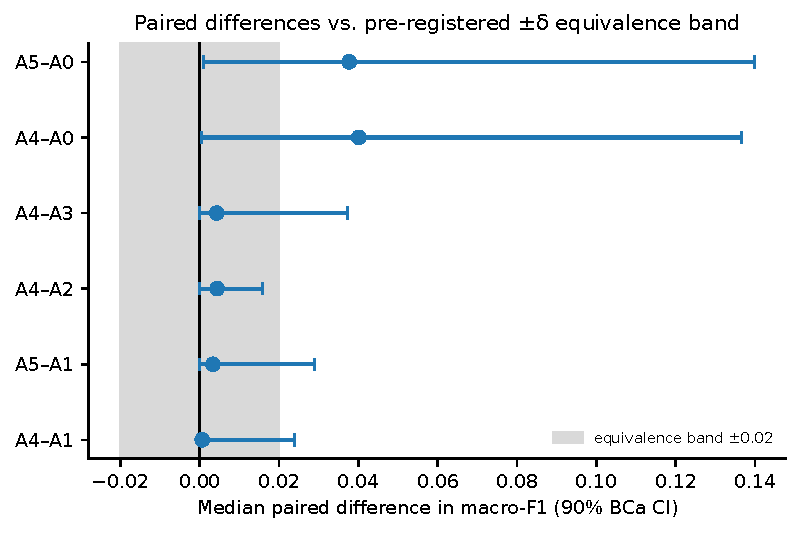
\includegraphics[width=0.82\textwidth]{fig05_paired_differences.pdf}
\caption{Planned paired comparisons: median paired \macrof{} difference with the
90\% BCa interval, against the pre-registered $\pm\delta$ equivalence band
($\delta = 0.02$). Encoder arms clear zero against the frozen model (A4--A0,
A5--A0); against maximum head-only replay (A4--A1, A5--A1) the intervals are
neither below the significance threshold after correction nor inside the
equivalence band---bounded but inconclusive.}
\label{fig:forest}
\end{figure}

\subsection{RQ3 --- Controlled replay-versus-plasticity ablations}

\textbf{Takeaway:} the encoder-plasticity contrast is statistically supported
(B4$-$B2, $p=0.005$, 16 of 21 patients improved), while replay \emph{volume} is
not; replay's clearest measured role is source retention, not target gain.

To separate replay location, replay volume, and trainable depth, we run the
B0--B7 controlled ablation matrix (Table~\ref{tab:causal_ablation},
Fig.~\ref{fig:causal}).
Arm means suggest a tidy story: adding raw replay to encoder LoRA lifts mean
\macrof{} from $0.755$ (B3, LoRA, no replay) to $0.803$ (B4, LoRA $+$ 62 raw), a
$+0.048$ apparent contribution of \emph{replay beyond plasticity}, while moving
from a frozen-encoder head at the same raw-replay budget (B2) to encoder LoRA
(B4) adds $+0.030$ from \emph{plasticity beyond replay}.

\paragraph{Only one of those two contributions survives paired testing.}
Differences of arm means are not evidence of a per-patient effect, so we test
each contrast patient-wise (Table~\ref{tab:causal_contrasts}). The plasticity
contrast is solid: B4$-$B2 gives $+0.030$ with a 95\% interval of
$[+0.007,+0.063]$ excluding zero, Wilcoxon $p = 0.005$, rank-biserial $0.74$, and
16 of 21 patients improved against 4 worsened. \textbf{The replay contrast is
not.} B4$-$B3 has a mean of $+0.048$ but a \emph{median of exactly zero}, an
interval $[-0.006,+0.112]$ that includes zero, $p = 0.473$, and a 10/11 split
between patients helped and harmed --- marginally more patients are \emph{worse}
with replay added than better. Its mean is carried by a handful of patients with
large gains, not by a consistent effect.

The two remaining contrasts sharpen the paper's central point. Replay
\emph{volume} does almost nothing: B1$-$B6 compares 705 post-pool exemplars
against 62 and yields $+0.008$ ($p = 0.232$) with only 5 patients improved and
\textbf{15 worsened} --- spending an extra 643 exemplars makes three times as
many patients worse as better. Encoder depth at matched post-pool volume
(B4$-$B7) is $+0.013$ and also not significant ($p = 0.179$).

We therefore state the controlled comparison result as: \emph{controlled ablations show a
statistically supported contribution from encoder plasticity, and a positive but
statistically unsupported mean contribution from replay, with no measurable
benefit from replay volume.} The earlier framing that replay and plasticity
``contribute independently'' overstated what the ablations establish, and we do
not use it. Replay's clearest measured role in this paper is not target gain at
all --- it is source retention, where its effect is large and consistent
(Section~\ref{sec:reg} and Section~\ref{sec:srcchange}).

\begin{table}[H]
\centering
\small
\caption{Paired uncertainty for the four controlled contrasts on the 21-record
patient-disjoint cohort, seeds averaged within patient. Arm means alone are
misleading here: only the \emph{plasticity} contrast is statistically supported.
``Mean''/``Med.'' are the paired difference, ``95\% CI'' a patient bootstrap
interval over the 21 patients ($10{,}000$ resamples), $p$ the Wilcoxon signed-rank value,
$r_{\mathrm{rb}}$ the rank-biserial effect size, ``I/W'' the threshold-free
improved/worsened split, and ``@$\epsilon$'' the same split at the $0.02$
threshold. B1, B4, and B7 are configuration-identical to A1, A4, and A2.}
\label{tab:causal_contrasts}
\setlength{\tabcolsep}{3pt}
\begin{tabular}{llrrcrrrr}
\toprule
Contrast & Interpretation & Mean & Med. & 95\% CI & $p$ & $r_{\mathrm{rb}}$ & I/W & @$\epsilon$ \\
\midrule
B4$-$B3 & replay beyond plast.      & $+0.048$ & $-0.000$ & $[-0.006,+0.112]$ & $0.473$ & $0.15$ & 10/11 & 6/4 \\
\textbf{B4$-$B2} & \textbf{plast.\ beyond replay} & $+0.030$ & $+0.006$ & $\mathbf{[+0.007,+0.063]}$ & $\mathbf{0.005}$ & $\mathbf{0.74}$ & \textbf{16/4} & 6/0 \\
B1$-$B6 & replay volume             & $+0.008$ & $-0.002$ & $[-0.027,+0.056]$ & $0.232$ & $0.37$ & 5/15 & 4/6 \\
B4$-$B7 & encoder depth             & $+0.013$ & $+0.003$ & $[-0.019,+0.043]$ & $0.179$ & $0.40$ & 14/6 & 8/4 \\
\bottomrule
\end{tabular}
\end{table}


\begin{table}[t]
\centering
\small
\caption{E9 controlled replay-versus-plasticity ablation matrix, recomputed on the
21-record patient-disjoint cohort (five seeds). \textbf{Arm means only} --- the
paired uncertainty that decides which contrasts are real is in
Table~\ref{tab:causal_contrasts}, and the mean differences here must not be read
as effects.}
\label{tab:causal_ablation}
\begin{tabular}{lllllll}
\toprule
ID & Status & Scope & Replay & Items & Mean & vs B1 \\
\midrule
B0 & complete & Frozen & none & 0 & 0.666 & $-0.119$ \\
B1 & complete & Head & postpool & 705 & 0.786 & $0.000$ \\
B2 & complete & Head & raw & 72 & 0.773 & $-0.013$ \\
B3 & complete & Encoder LoRA rank 1 & none & 0 & 0.755 & $-0.031$ \\
B4 & complete & Encoder LoRA rank 1 & raw & 62 & 0.803 & $+0.017$ \\
B5 & infeasible & Encoder LoRA rank 1 & raw & 72 &  &  \\
B6 & complete & Head & postpool & 62 & 0.778 & $-0.008$ \\
B7 & complete & Post-pool adapter rank 1 & postpool & 678 & 0.790 & $+0.004$ \\
\bottomrule
\end{tabular}
\end{table}


\begin{figure}[H]
\centering
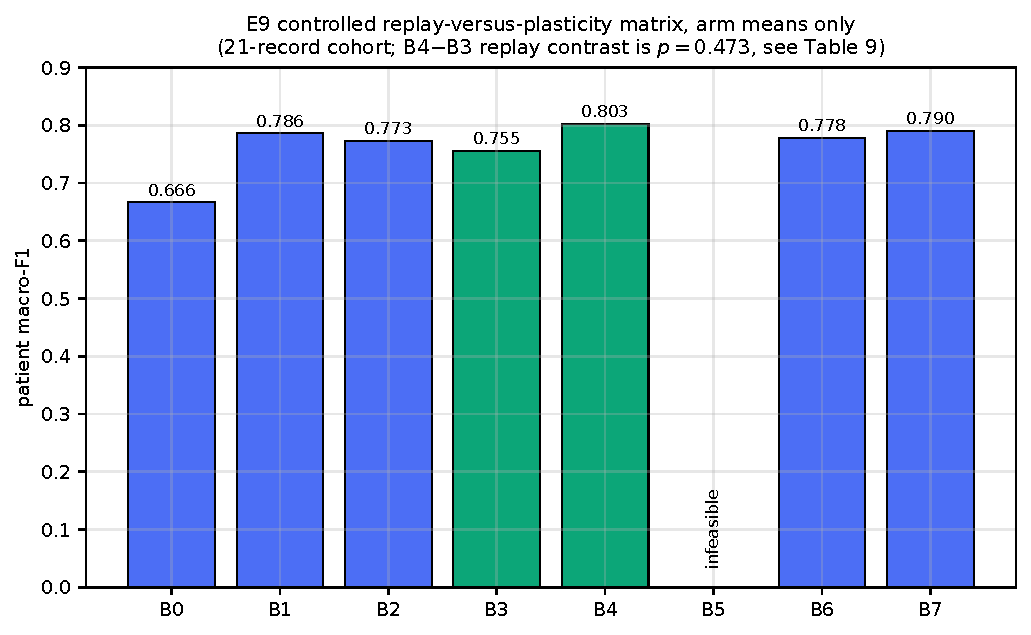
\includegraphics[width=0.86\textwidth]{fig_causal_ablation.pdf}
\caption{Replay-versus-plasticity ablation, arm means only. The apparent
ordering B4$>$B3 (replay added) and B4$>$B2 (plasticity added) is what mean
differences suggest, but \textbf{only the plasticity contrast survives paired
testing}: B4$-$B2 has $p = 0.005$ while B4$-$B3 has $p = 0.473$ with a median of
essentially zero and a 10/11 patient split. Read this figure together with
Table~\ref{tab:causal_contrasts}, which carries the uncertainty; the bars alone
overstate the replay effect.}
\label{fig:causal}
\end{figure}

\subsection{Can regularization substitute for replay?}
\label{sec:reg}

\textbf{Takeaway:} replay provides substantially better source retention than the
tested zero-byte $B$-factor anchor under the evaluated configuration --- at
matched bytes the anchor loses about five times as much source performance as
replay while adapting less. One regularizer was tested, so this is not a
statement about regularization in general.

\paragraph{What this does and does not say about EWC-LoRA.} The closest
published method is EWC-LoRA \cite{zheng2026ewclora}, which applies a
Fisher-based penalty to a shared low-rank update for task-sequential continual
learning. \textbf{We do not implement it}, so nothing here should be read as a
comparison against it. Two differences make a direct transfer non-obvious rather
than merely untested: their setting accumulates \emph{tasks} while ours is
constrained by \emph{bytes}, and a Fisher importance estimate is persistent
state that would itself have to be charged against the 16\,KiB ceiling --- a
diagonal Fisher over even the 223 trainable parameters of A4 is small, but over
the full 6{,}643-parameter model it is not (Section~\ref{sec:relatedwork}).
Evaluating EWC-LoRA under a byte budget is the single most relevant extension of
the regularization arm of this study, and we flag it as such rather than
claiming the question is closed.

The arms compared so far are all replay-based, which leaves open whether the
budget would be better spent on a regularizer than on stored exemplars. The
classical answer, elastic weight consolidation, is infeasible here: a full-model
FP32 parameter anchor plus a Fisher value costs $6643 \times 8 = 53{,}144$\,B,
more than three times the entire budget before a single exemplar is stored.

A low-rank adapter admits a much cheaper anchor. The attention delta is $(xA)B$
with $B$ zero-initialised, so shrinking $B$ pulls the adapted model back toward
the frozen source function, and it costs \textbf{zero persistent bytes} because
the anchor \emph{is} the frozen base weight the device already stores for
inference. The implemented penalty is
\begin{equation}
\mathcal{L}_{\mathrm{reg}} = \lambda \sum_{m \in \{q,k,v,o\}} \|B_m\|_F^2,
\qquad \lambda = 10^{-2},
\label{eq:anchor}
\end{equation}
applied to the $B$ factor of each of the four attention projections. We state one
caveat plainly, because it bounds the interpretation: the quantity that actually
determines the function is the product $A_mB_m$, and since
$A_mB_m = (cA_m)(B_m/c)$, penalising $B_m$ alone constrains the
\emph{parametrisation} rather than the function. $\|A_mB_m\|_F^2$ is the
better-posed penalty; Eq.~\eqref{eq:anchor} is what was run, and we report it as
such rather than describing it as a direct penalty on the source-function
deviation. This is therefore \textbf{a low-cost memory-matched regularization
baseline}, not the strongest regularizer the budget admits --- restricted EWC on
the adapter parameters, source-logit distillation, and output-consistency
regularization all remain untested. We add two arms: R1 (rank-1 LoRA, anchor, no
replay), byte-comparable with B3, and R2 (rank-1 LoRA, anchor, 62 raw exemplars),
byte-identical to A4.

The answer is clear in both directions (Table~\ref{tab:regularization}).
\emph{As a substitute for replay, the anchor is weak.} Without replay it trades a
little target gain for a little stability relative to unregularized LoRA
($0.755 \to 0.744$ target, $\Delta^{\mathrm{src}}$ $-0.159 \to -0.136$). Replay achieves far
more on both axes at once: A4 reaches $+0.136$ target gain against R1's $+0.078$,
and holds the source-domain change to $-0.027$ against R1's $-0.136$, so the anchor loses
about five times as much source performance as replay does, while also adapting
less. \emph{As a
complement to replay, the anchor is redundant.} R2 is statistically
indistinguishable from A4 on target performance ($0.803$ versus $0.803$) and
improves $\Delta^{\mathrm{src}}$ only from $-0.027$ to $-0.023$.

We take two things from this, both hedged by the caveat above. First, the paper's
replay-centric framing is not an untested assumption: at this scale, stored source
exemplars regulate stability substantially better than this parameter-space
penalty does, which is what one would expect when the shift is a change of patient
rather than a change of task. Second, the anchor is nearly free, so R2 remains a
reasonable default for a deployment wanting the small extra retention margin at no
byte cost. Because only one regularizer was tested, and in its scale-ambiguous
form, we claim only that \emph{this} anchor does not substitute for replay --- not
that regularization in general cannot.

\begin{table}[H]
\centering
\small
\caption{Memory-matched regularization baseline on the 21-record patient-disjoint
cohort (5 seeds). The source anchor is $\lambda\sum_m\|B_m\|_F^2$ on the $B$
factor of each attention projection (Eq.~\ref{eq:anchor}); because $B$ is
zero-initialised and the frozen base weights \emph{are} the anchor, it costs
\textbf{zero persistent bytes}, so R1 is byte-comparable with B3 and R2 with A4.
Penalising $B$ rather than the product $AB$ is scale-ambiguous and constrains the
parametrisation rather than the function; this is a low-cost baseline, not the
strongest regularizer available. $\Delta^{\mathrm{src}}$ is the signed
source-domain \macrof{} change.}
\label{tab:regularization}
\setlength{\tabcolsep}{4pt}
\begin{tabular}{llccrrrr}
\toprule
Arm & Mechanism & Replay & Anchor & Bytes & \macrof{} & $\Delta$ vs.\ A0 & $\Delta^{\mathrm{src}}$ \\
\midrule
A0 & frozen                    & ---  & ---  & 0        & 0.666 & ---                        & $0.000$ \\
B3 & LoRA $r{=}1$              & ---  & ---  & 3{,}568  & 0.755 & $+0.089$ ($p=0.044$)       & $-0.159$ \\
R1 & LoRA $r{=}1$ $+$ anchor   & ---  & yes  & 3{,}568  & 0.744 & $+0.078$ ($p=0.052$)       & $-0.136$ \\
A4 & LoRA $r{=}1$ $+$ replay   & 62   & ---  & 16{,}208 & 0.803 & $+0.136$ ($p=0.0012$)      & $\mathbf{-0.027}$ \\
R2 & LoRA $r{=}1$ $+$ both     & 62   & yes  & 16{,}208 & \textbf{0.803} & $\mathbf{+0.137}$ ($p=0.0011$) & $-0.023$ \\
\bottomrule
\end{tabular}
\end{table}


\subsection{RQ4 --- Adam budget sweep for rank-1 and rank-2 adaptation}
\label{sec:rq4}

\textbf{Takeaway:} within the measured 12-record Adam rank-1/rank-2 panel,
raising the adaptation-state budget from 8 to 64\,KiB produced no statistically
detectable benefit (secondary evidence, reduced panel). We do not generalize
beyond the panel that was measured.

The primary study fixes a single 16\,KiB budget, which raises the obvious
question of whether the conclusions are an artifact of that particular point. The
experiment that speaks to it, E10, was designed as a full budget $\times$
optimizer $\times$ rank grid but was executed only in part, so we name it for
what was actually measured: an \textbf{Adam budget sweep for rank-1 and rank-2
adaptation} at 8, 16, 32, and 64\,KiB. The unmeasured dimensions are not
discussed as results anywhere in this paper.

\paragraph{Scope, stated up front.} This sweep is \textbf{secondary evidence and
is not comparable to the primary cohort}. Two limitations must be read before the
numbers. First, to keep the grid tractable it was executed on a reduced panel of
\textbf{12 DS2 records and 3 seeds} (864 adaptation cells), not the 21-record,
5-seed primary cohort; absolute values are therefore not interchangeable with
Table~\ref{tab:primary_arms}, and no cell of this sweep may be ranked against a
primary-cohort arm. Second, the executed grid is a \emph{subset} of the planned
design: 49 of 140 planned configurations are measured, 5 are analytically
infeasible at their budget, and 86 remain unrun. The budget $\times$ scope
$\times$ rank surface is complete \emph{only for Adam at ranks 1 and 2}; SGD is
measured at 8\,KiB alone, SGD-with-momentum not at all, and ranks 4 and 8 are
almost entirely unmeasured (rank 8 is infeasible at 8 and 16\,KiB by the memory
model).

The single claim this experiment supports is therefore narrow and we state it
once, here: \emph{within the measured Adam rank-1/rank-2 panel, no statistically
resolvable improvement was observed when increasing the persistent-state budget
from 8 to 64\,KiB.} We make \textbf{no optimizer-ranking claim, no rank-4 or
rank-8 claim, and no claim that the 140-cell design is complete.}

\paragraph{Result: no detectable benefit above 8\,KiB.} Within the Adam panel
(Table~\ref{tab:e10_adam}, Fig.~\ref{fig:saturation}), raising the budget from 8
to 64\,KiB does not improve per-patient \macrof{} for any family. The encoder-LoRA
family is flat-to-declining ($0.805 \to 0.790 \to 0.776 \to 0.768$), the
post-pool-adapter family varies within $0.762$--$0.780$, and the head-only family
within $0.762$--$0.774$.

Overlapping confidence intervals are not evidence of equivalence, so we test the
budget effect directly. Holding optimizer, trainable scope, rank, and replay
location fixed and varying \emph{only} the budget gives a paired contrast on each
record; we test each with a Wilcoxon signed-rank test and, for equivalence, with
a two-one-sided-tests (TOST) procedure against a margin of $\delta = 0.05$
\macrof{} stated before analysis (Table~\ref{tab:e10_paired}). Of the 18
budget contrasts, \textbf{14 met the pre-specified $\pm 0.05$ equivalence
criterion} against their 8\,KiB reference, and none of the raises is
significantly positive.

\paragraph{Why $\delta = 0.05$, and what the 18 decisions are not.} The margin
was fixed before analysis at $0.05$ \macrof{} because it is roughly a third of
the primary adaptation effect this paper is built on (A4$-$A0 $= +0.136$): a
budget change that moves \macrof{} by less than $\delta$ cannot account for the
adaptation gain, which is the question the sweep exists to answer. It is a
within-panel yardstick, not a claim about clinical meaningfulness, and it is
coarser than the $\epsilon = 0.02$ per-patient harm threshold used in RQ2
because the sweep panel has 12 records rather than 21 and correspondingly wider
intervals. \textbf{The 18 TOST decisions are not multiplicity-adjusted.} They
sit outside the six-comparison Holm family, which was reserved for the primary
analysis, so each equivalence decision is an uncorrected per-contrast statement
and the count ``14 of 18'' should be read descriptively. Adjusting would make
equivalence harder to declare, not easier, so the direction of the resulting
bias is toward over-claiming equivalence --- another reason we keep the claim
inside the measured panel.

Two contrasts deserve explicit mention because they cut against a naive
``more memory is at least harmless'' reading. For rank-2 encoder LoRA, moving
from 8 to 64\,KiB \emph{significantly reduces} \macrof{} by $0.039$
(Wilcoxon $p = 0.003$), and the 32\,KiB contrast is also negative
($-0.027$, $p = 0.027$); neither is equivalent within the margin. The likely
mechanism is that a raw-replay buffer of several hundred source exemplars starts
to dominate a 500-beat target set, pulling the adapted model back toward the
source. We report this as a measured effect on the secondary panel rather than a
general law.

The defensible reading is a null result of a useful kind, stated at the scope it
was measured: \emph{within the measured 12-record Adam rank-1/rank-2 panel,
increasing the adaptation-state budget produced no statistically detectable
benefit, and for rank-2 encoder LoRA it produced a detectable cost}. On that
panel, extra persistent memory did not buy accuracy, which is consistent with
the allocation question studied in RQ2 and RQ3 --- how to spend a fixed budget
--- being the one that matters. We do not extend this to unmeasured optimizers,
ranks, or cohorts, and we do not claim that 16\,KiB is provably sufficient in
general.

\paragraph{A separate low-byte measurement.}\label{sec:lowbyte} Independently of this sweep, a
fixed-scope run on the \emph{full} 22-record, 5-seed cohort measured a rank-1
encoder-LoRA configuration holding only \textbf{8 raw replay samples} in
$5{,}246$\,B --- under a third of the budget --- reaching $0.801$ per-patient
\macrof{} on the contaminated 22-record cohort, against $0.802$ for the 16\,KiB
rank-2 arm (A5) on the same cohort. We quote this pair on the 22-record basis
because that fixed-scope run was not repeated after the cohort correction.
\textbf{It is therefore a historical sensitivity result and is \emph{not}
directly comparable with Table~\ref{tab:primary_arms}}, which is computed on the
corrected 21-record cohort; the two numbers quoted here are internally
comparable with each other and with nothing else in this paper. Read only within
itself, the pair is suggestive of the same saturation direction --- a
third-of-budget configuration landing beside a full-budget one --- but it carries
no weight against any primary-cohort figure.

\begin{table}[H]
\centering
\small
\caption{Adam budget sweep, rank-1 and rank-2 (E10): best configuration per family at each budget
(per-patient \macrof{}, N/S/V present classes). \textbf{Reduced secondary panel
of 12 DS2 records and 3 seeds, Adam only, ranks 1 and 2 --- not comparable to the
primary cohort of Table~\ref{tab:primary_arms}.} SGD and SGD-with-momentum cells
are excluded as unmeasured (except 8\,KiB SGD). Formal budget contrasts and
equivalence decisions are in Table~\ref{tab:e10_paired}; the means here are
descriptive and should not be read as a ranking.}
\label{tab:e10_adam}
\begin{tabular}{lrrrr}
\toprule
Family & 8\,KiB & 16\,KiB & 32\,KiB & 64\,KiB \\
\midrule
Encoder LoRA $+$ raw replay        & \textbf{0.805} & \textbf{0.790} & 0.776 & \textbf{0.768} \\
Post-pool adapter $+$ post-pool    & 0.762 & 0.765 & \textbf{0.780} & 0.767 \\
Head only                          & 0.762 & 0.774 & 0.765 & 0.763 \\
\bottomrule
\end{tabular}
\end{table}

% GENERATED FILE -- do not edit by hand.
% Regenerate with: make tables  (scripts/make_tables.py)
\begin{table}[H]
\centering
\small
\caption{Paired budget contrasts within the Adam rank-1/rank-2 sweep (E10). Optimizer, trainable scope, rank, and replay location are held fixed and only the budget varies, so each row is a paired comparison over the same 12 records of the secondary panel (3 seeds, Adam only). $\Delta$ is the mean paired change in per-patient \macrof{} relative to the same configuration at 8\,KiB. ``Equiv.'' is a TOST equivalence decision at the pre-stated margin $\delta = 0.05$. 14 of 18 contrasts are equivalent. Raising the budget is never significantly beneficial; for rank-2 encoder LoRA at 64\,KiB it is significantly harmful.}
\label{tab:e10_paired}
\setlength{\tabcolsep}{5pt}
\begin{tabular}{llcrrcc}
\toprule
Scope & Replay & Rank & Budget & $\Delta$ vs.\ 8\,KiB & Wilcoxon $p$ & Equiv. \\
\midrule
\multirow{3}{*}{Encoder LoRA} & \multirow{3}{*}{raw} & \multirow{3}{*}{1} & 16\,KiB & $+0.015$ & $0.204$ & yes \\
 & & & 32\,KiB & $+0.007$ & $0.424$ & yes \\
 & & & 64\,KiB & $+0.002$ & $0.380$ & yes \\
\midrule
\multirow{3}{*}{Encoder LoRA} & \multirow{3}{*}{raw} & \multirow{3}{*}{2} & 16\,KiB & $-0.013$ & $0.164$ & yes \\
 & & & 32\,KiB & $-0.027$ & $\mathbf{0.027}$ & yes \\
 & & & 64\,KiB & $-0.039$ & $\mathbf{0.003}$ & no \\
\midrule
\multirow{3}{*}{Head only} & \multirow{3}{*}{post-pool} & \multirow{3}{*}{0} & 16\,KiB & $+0.006$ & $0.577$ & yes \\
 & & & 32\,KiB & $+0.004$ & $0.898$ & yes \\
 & & & 64\,KiB & $+0.003$ & $0.831$ & yes \\
\midrule
\multirow{3}{*}{Head only} & \multirow{3}{*}{raw} & \multirow{3}{*}{0} & 16\,KiB & $+0.000$ & $0.519$ & yes \\
 & & & 32\,KiB & $-0.004$ & $0.677$ & yes \\
 & & & 64\,KiB & $+0.010$ & $0.776$ & no \\
\midrule
\multirow{3}{*}{Post-pool adapter} & \multirow{3}{*}{post-pool} & \multirow{3}{*}{1} & 16\,KiB & $+0.016$ & $0.240$ & yes \\
 & & & 32\,KiB & $+0.030$ & $0.519$ & no \\
 & & & 64\,KiB & $+0.017$ & $0.831$ & no \\
\midrule
\multirow{3}{*}{Post-pool adapter} & \multirow{3}{*}{post-pool} & \multirow{3}{*}{2} & 16\,KiB & $-0.001$ & $1.000$ & yes \\
 & & & 32\,KiB & $+0.007$ & $0.519$ & yes \\
 & & & 64\,KiB & $+0.006$ & $1.000$ & yes \\
\bottomrule
\end{tabular}

\vspace{0.4em}
{\small A contrast can be \emph{both} significantly different from zero and statistically equivalent within $\pm 0.05$: rank-2 encoder LoRA at 32\,KiB is one (Wilcoxon $p = 0.027$, TOST $p = 0.027$). Significance asks whether the difference is distinguishable from zero; equivalence asks whether it is small. The two columns answer different questions and must not be read as each other's complement. The 18 decisions are \textbf{not} multiplicity-adjusted.}
\end{table}


\begin{figure}[H]
\centering
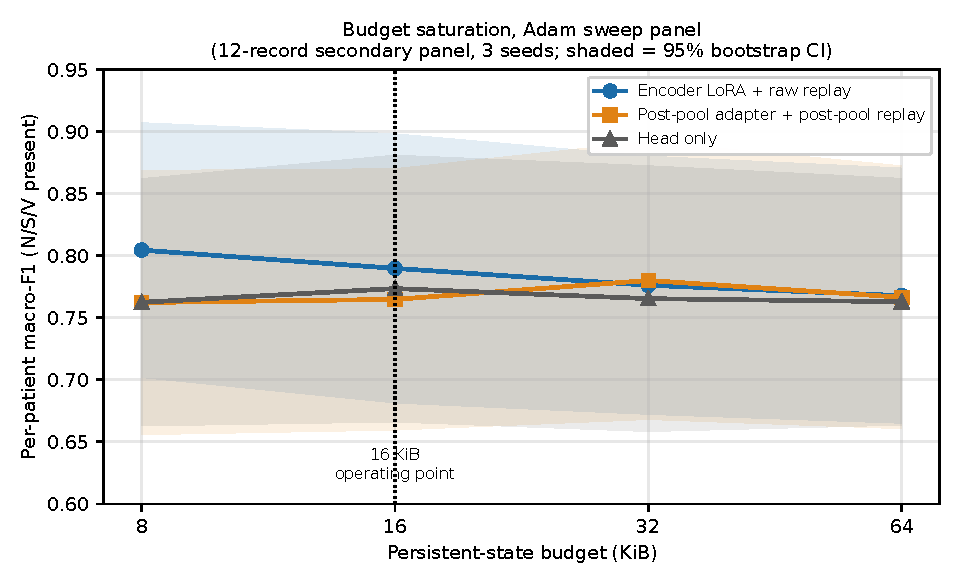
\includegraphics[width=0.80\textwidth]{fig_e10_budget_saturation.pdf}
\caption{Per-patient \macrof{} versus persistent-state budget for the Adam
rank-1/rank-2 sweep (E10). \textbf{Secondary cohort: 12 DS2 records, 3 seeds, Adam only, ranks 1 and
2; not directly comparable to Table~\ref{tab:primary_arms}.} Points are the best
configuration per family at each budget and shaded bands are 95\% bootstrap
intervals over records. The bands overlap, but overlap alone is not evidence of
equality --- the supporting claim is the paired TOST analysis of
Table~\ref{tab:e10_paired}, in which 14 of 18 budget contrasts are equivalent
within $\pm 0.05$ \macrof{} and none is significantly positive.}
\label{fig:saturation}
\end{figure}

\subsection{Does the result depend on spending the last kilobyte?}
\label{sec:reserve}

\textbf{Takeaway:} the result does not depend on saturating the budget ---
reserving 1\,KiB and regenerating replay counts leaves every adapted arm
significantly above frozen ($p\le0.010$) with encoder adaptation still among the
top allocations.

Every configuration reported so far fills the 16\,KiB budget almost exactly ---
A2 reaches $16{,}383$ of $16{,}384$ bytes. That is not a deployable margin: real
firmware needs room for a version field, a checksum, and future additions, and a
configuration generated against a ceiling it exactly saturates would break the
moment anything is added. We therefore re-ran the entire A0--A5 grid, same 21
records and five seeds, against an effective ceiling of
$B_{\mathrm{budget}} - B_{\mathrm{reserve}} = 16{,}384 - 1{,}024 = 15{,}360$\,B,
regenerating replay counts rather than reporting old results against new byte
figures. The reserve costs A1 49 exemplars, A4 five, and A5 five
(Table~\ref{tab:arm_definitions}).

The qualitative conclusion is preserved (Table~\ref{tab:reserve}): every adapted
arm remains significantly above the frozen model ($p \le 0.010$), encoder
adaptation remains among the top-performing allocations, and A4 is unchanged at
$0.802$. The \emph{exact} arm ordering is not preserved, and we say so rather
than claiming otherwise: without the reserve the order is
$\mathrm{A5} > \mathrm{A4} > \mathrm{A2} > \mathrm{A1} > \mathrm{A3}$, and with it
$\mathrm{A4} > \mathrm{A1} > \mathrm{A5} > \mathrm{A2} > \mathrm{A3}$. A1 gains
slightly ($0.786 \to 0.793$) while A5 loses more ($0.809 \to 0.792$). A5 is thus
more sensitive than A4 to losing the last few replay samples, which supports
\textbf{rank-1 encoder LoRA as the more robust engineering operating point} --- a
practical conclusion the unreserved analysis alone would have missed. We keep the unreserved configuration as the primary analysis because it
is what the pre-specified plan defined, and report the reserve replication as the
deployable-margin check. \textbf{The primary statistical conclusion is
unchanged, although the exact ordering and the preferred engineering operating
point change under the reserve.}

\begin{table}[H]
\centering
\small
\caption{Implementation-reserve replication on the 21-record patient-disjoint
cohort. The full A0--A5 grid re-run against an effective ceiling of
$15{,}360$\,B, i.e.\ holding back a 1\,KiB firmware reserve, same records and
five seeds. Replay counts fall by roughly $7$--$8\%$. Every arm still
significantly beats the frozen model and encoder adaptation stays among the top
allocations, though the exact ordering changes: A5 loses more than A4, making
rank-1 the more robust operating point. \emph{Values are seeds mean-averaged
within patient; median unification of this secondary replication is deferred
(see \texttt{BLOCKERS.md}, ESC-4).}}
\label{tab:reserve}
\setlength{\tabcolsep}{5pt}
\begin{tabular}{lrrrrrr}
\toprule
& \multicolumn{3}{c}{16{,}384\,B ceiling} & \multicolumn{3}{c}{$15{,}360$\,B ceiling ($+1$\,KiB reserve)} \\
\cmidrule(lr){2-4}\cmidrule(lr){5-7}
Arm & Items & \macrof{} & $\Delta$ vs.\ A0 & Items & \macrof{} & $\Delta$ vs.\ A0 \\
\midrule
A0 & 0   & 0.666 & ---      & 0   & 0.666 & --- \\
A1 & 705 & 0.786 & $+0.119$ & 656 & 0.793 & $+0.127$ \\
A2 & 678 & 0.790 & $+0.124$ & 629 & 0.779 & $+0.113$ \\
A3 & 650 & 0.775 & $+0.109$ & 601 & 0.771 & $+0.105$ \\
A4 & 62  & 0.803 & $+0.136$ & 57  & \textbf{0.802} & $\mathbf{+0.136}$ \\
A5 & 52  & \textbf{0.809} & $\mathbf{+0.143}$ & 47 & 0.792 & $+0.125$ \\
\bottomrule
\end{tabular}

\vspace{0.4em}
{\small All reserve-arm gains over A0 remain significant by paired Wilcoxon
($p = 0.006$, $0.003$, $0.010$, $0.004$, $0.005$ for A1--A5). Unreserved the
order is $\mathrm{A5}>\mathrm{A4}>\mathrm{A2}>\mathrm{A1}>\mathrm{A3}$; reserved
it is $\mathrm{A4}>\mathrm{A1}>\mathrm{A5}>\mathrm{A2}>\mathrm{A3}$.}
\end{table}


\subsection{Does the boundary filter dependency matter?}
\label{sec:splitfirst}

\textbf{Takeaway:} no. Removing the dependency entirely moves every arm mean by
at most $0.007$ \macrof{}, leaves both encoder-versus-frozen contrasts
significant at $p = 0.0012$, and leaves both encoder-versus-A1 contrasts
non-significant. The conclusions are not artifacts of non-causal preprocessing.

The released preprocessing filters each record as a whole before the
chronological split (Section~\ref{sec:protocol}), so adaptation-side samples
within the filters' backward reach of the boundary can depend on test-segment raw
samples. To remove that dependency rather than argue about its size, we rebuilt
the beat store \emph{split-first}: the raw signal is cut at the boundary, a
$720$-sample ($2$\,s) guard is discarded from each side --- roughly a sixfold
margin on the measured $120$-sample influence reach --- and the two pieces are
filtered independently, so no adaptation-side sample can see a test-side raw
sample. Beats whose window would straddle the cut are dropped, which costs one to
three adaptation beats per record; we then truncate every record to a uniform
$497$-beat adaptation block so the protocol stays balanced.

We reran A0, A1, A4, and A5 on this store over the same 21 patient-disjoint
records and the same five seeds. Table~\ref{tab:splitfirst} reports the result.

Three things are worth separating. First, the \textbf{frozen arm is unmoved}
($-0.0000$, largest per-record shift $0.0004$). A0 performs no adaptation, so it
isolates the effect of refiltering the test segment alone, and that effect is
numerically negligible --- which is the expected result and a useful check that
the rebuild did not perturb the evaluation data.

Second, the \textbf{adapted arms move very little, and not in the direction
leakage would predict}. A1 rises by $0.007$, A4 falls by $0.006$, and A5 is
unchanged to three decimals. If whole-record filtering had been inflating the
results, removing it should have lowered them systematically; instead the shifts
have mixed sign. \textbf{The seeds are identical across the two runs, so these
are not run-to-run fluctuations.} They reflect the combined effects of the three
things the rerun actually changes: independent segment filtering, removal of
boundary-adjacent beats, and reducing the adaptation block from $500$ to $497$
labelled beats. Their magnitude is too small to alter any inferential
conclusion.

Third, and most importantly, \textbf{no inferential conclusion changes}.
Table~\ref{tab:splitfirst_contrasts} recomputes the four contrasts that matter
on the split-first cohort, reporting both raw and family-corrected $p$-values.
These four form their own sensitivity family and are \emph{not} pooled with the
six pre-specified primary comparisons. Both
encoder arms remain significantly above the frozen model on the split-first
cohort (under the locked estimator A4 improves $16/21$ patients and A5 $17/21$;
the arm \macrof{} in Table~\ref{tab:splitfirst} is seeds mean-averaged, ESC-4),
and the two comparisons against maximum
head-only replay remain non-significant, so the paper's central refusal to claim
superiority over A1 is unaffected. The one substantive change is that the
\emph{margin} over A1 shrinks --- A4$-$A1 falls from $+0.017$ to $+0.004$ and
A5$-$A1 from $+0.023$ to $+0.017$ --- which weakens the encoder-over-head
ordering slightly rather than strengthening it. We report that in the direction
it points: the split-first evidence makes the frontier reading \emph{more}
appropriate, not less.

This is a sensitivity analysis, not a replacement primary analysis. The headline
numbers throughout the paper remain those of the released pipeline, so that they
correspond to the pre-specified plan and to the published artifacts; the
split-first rerun is reported here as the check that the boundary dependency
does not carry the result. A fully causal streaming front end --- which would
also have to replace the zero-phase filter, not merely the record boundary ---
remains future work.

% GENERATED FILE -- do not edit by hand.
% Regenerate with: make tables  (scripts/make_tables.py)
\begin{table}[H]
\centering
\small
\caption{Boundary-leakage sensitivity (E17). The split-first rerun cuts the raw signal at the boundary, discards a $2$\,s guard each side, and filters the pieces independently, so no adaptation-side sample can depend on a test-side raw sample. \textbf{Every conclusion is preserved.}}
\label{tab:splitfirst}
\begin{tabular}{lrrr}
\toprule
Arm & Whole-record & Split-first & $\Delta$ \\
\midrule
A0 (frozen) & $0.666$ & $0.666$ & $-0.000$ \\
A1 (head $+$ max replay) & $0.786$ & $0.793$ & $+0.007$ \\
A4 (LoRA $r{=}1$) & $0.803$ & $0.796$ & $-0.006$ \\
A5 (LoRA $r{=}2$) & $0.809$ & $0.809$ & $+0.000$ \\
\bottomrule
\end{tabular}
\end{table}


% GENERATED FILE -- do not edit by hand.
% Regenerate with: make tables  (scripts/make_tables.py)
\begin{table}[H]
\centering
\small
\caption{Paired contrasts recomputed on the split-first (E17) cohort, $n = 21$ patients, five seeds averaged within patient. \textbf{These four sensitivity contrasts form their own family and are not pooled with the six pre-specified primary comparisons}; the Holm column corrects within these four only. Both frozen-model contrasts remain significant and neither encoder arm clears maximum head-only replay, matching the primary cohort.}
\label{tab:splitfirst_contrasts}
\setlength{\tabcolsep}{4pt}
\begin{tabular}{lrrcrrr}
\toprule
Contrast & Mean $\Delta$ & Med. $\Delta$ & 95\% CI & Raw $p$ & Holm $p$ & Impr./Wors. \\
\midrule
\textbf{A4$-$A0} & $+0.130$ & $+0.040$ & $[+0.050,+0.231]$ & $0.0012$ & \textbf{$0.0047$} & 17 / 4 \\
\textbf{A5$-$A0} & $+0.143$ & $+0.039$ & $[+0.060,+0.245]$ & $0.0012$ & \textbf{$0.0047$} & 17 / 4 \\
A4$-$A1 & $+0.004$ & $+0.001$ & $[-0.021,+0.027]$ & $0.3135$ & $0.4359$ & 14 / 6 \\
A5$-$A1 & $+0.017$ & $+0.001$ & $[-0.014,+0.047]$ & $0.2180$ & $0.4359$ & 14 / 6 \\
\bottomrule
\end{tabular}

\vspace{0.4em}
{\small ``Raw $p$'' is the unadjusted paired Wilcoxon signed-rank value; ``Holm $p$'' corrects across these four sensitivity contrasts. Intervals are patient bootstraps ($10{,}000$ resamples).}
\end{table}



\subsection{RQ5 --- Robustness to alternative class-reweighted source checkpoints}

\textbf{Takeaway:} the adaptation gain persists under two alternative
class-reweighted source-training objectives. This supports robustness to the
source \emph{objective}, but does \textbf{not} establish robustness to a
\emph{stronger unseen-patient source model}, which was never demonstrated
(secondary evidence).

A key robustness question is whether the adaptation gain merely corrects an
unusually weak S-class source. We train five architecture-identical source
variants on MIT--BIH DS1 with five seeds---cross-entropy, effective-number class
weighting, and focal loss $\gamma\in\{1,2,3\}$---and measure them under the same
protocol (Table~\ref{tab:e11_source_status}).

\paragraph{We do not call these checkpoints stronger, because on the reported
metric they are not.} Intra-patient DS1 S sensitivity is $0.881$ for plain
cross-entropy, $0.843$ for focal $\gamma{=}2$, and $0.776$ for effective-number
weighting: the class-reweighted objectives are \emph{below} the cross-entropy
baseline on exactly the axis that motivated the concern, and they also cost
overall \macrof{}. Calling them \emph{stronger source checkpoints} would not be
supported by these results, so we describe them for what they are ---
\textbf{alternative source checkpoints trained with class-reweighted
objectives} --- and treat RQ5 as a test of whether the adaptation result is
\emph{robust to the choice of source objective}, not as adaptation from a
stronger starting point.

One further caution: the S sensitivities above are measured on an intra-patient
DS1 split, whereas the frozen-source weakness that motivates adaptation is an
unseen-patient DS2 property. These are different domains and we do not compare
them as if they were the same. Establishing which checkpoint is genuinely
stronger on unseen patients would require evaluating every variant frozen on DS2,
which we have not done; that is the experiment RQ5 would need to make a true
stronger-source claim.

Training five variants is not the same as adapting from five, and we separate
the two explicitly: all five variants were \emph{trained} and measured for source
quality (Table~\ref{tab:e11_source_status}), while adaptation was re-run from
\textbf{two} of them --- effective-number weighting and focal $\gamma{=}2$, the
two that most change the minority-class behaviour the concern is about
(Table~\ref{tab:strong_adapt}). The gain survives: adapting from the
effective-number source lifts per-patient \macrof{} (N/S/V) from $0.458$ (frozen)
to $0.599$ (both head-only and encoder LoRA), and from the focal-$\gamma{2}$
source from $0.515$ to $0.642$ (head) and $0.644$ (encoder LoRA). On the
encoder-versus-head question these two runs say less than they appear to:
\emph{the mean encoder-minus-head direction remains nonnegative under two
alternative class-reweighted source objectives, but the margins are small
($+0.0001$ and $+0.0024$) and no uncertainty is reported}, so they are
consistent with the primary-cohort finding of a non-significant direct
comparison rather than independent support for an ordering.
Adaptation from the remaining three trained
variants (cross-entropy and focal $\gamma \in \{1,3\}$) is not reported here, so
we claim only that \emph{the ordering was re-evaluated from two
class-reweighted source checkpoints}, not from five. The three RR-architecture
and CNN variants require new model graphs and were never trained; they are
labeled \texttt{not\_implemented\_not\_run} in the ledger.

\begin{table}[H]
\centering
\small
\caption{E11 source-checkpoint ledger. All five variants share the architecture of
the shipped backbone and differ only in the training objective; each is trained on
MIT--BIH DS1 with five seeds and scored on a held-out \emph{intra-patient} DS1
split. The right-hand column separates the checkpoints we \emph{trained} from
those we also \emph{adapted from}, because the robustness claim covers only the
latter. \textbf{None of the reweighted objectives beats plain cross-entropy on S
sensitivity} ($0.881$), so we do not describe them as stronger sources; RQ5 tests
robustness to the source objective, not adaptation from a better starting point.
These intra-patient DS1 figures are also not comparable to unseen-patient DS2
behaviour.}
\label{tab:e11_source_status}
\begin{tabular}{llrrc}
\toprule
Source variant & Status & \macrof{} & S sens. & Adapted from? \\
\midrule
Cross-entropy (\texttt{original\_ce})   & measured, 5 seeds & \textbf{0.742} & \textbf{0.881} & no \\
Effective-number weighting              & measured, 5 seeds & 0.618 & 0.776 & \textbf{yes} \\
Focal loss $\gamma = 1$                 & measured, 5 seeds & 0.741 & 0.878 & no \\
Focal loss $\gamma = 2$                 & measured, 5 seeds & 0.730 & 0.843 & \textbf{yes} \\
Focal loss $\gamma = 3$                 & measured, 5 seeds & 0.725 & 0.780 & no \\
\midrule
RR-conditioned token embedding          & not implemented   & ---   & ---   & --- \\
RR token before attention               & not implemented   & ---   & ---   & --- \\
Lightweight inter-patient CNN           & not implemented   & ---   & ---   & --- \\
\bottomrule
\end{tabular}

\vspace{0.4em}
{\small The three unimplemented rows require new model graphs and were never
trained; they are recorded here rather than omitted so the ledger matches the
experiment plan. Three further pre-existing \texttt{beat\_classifier} checkpoints
exist in the repository but were measured on an intra-patient random split rather
than the DS1-only protocol, so they are not comparable and are excluded from this
table.}
\end{table}


\begin{table}[H]
\centering
\small
\caption{Adaptation from two E11 class-reweighted source checkpoints
(per-patient \macrof{} over N/S/V, DS2, five seeds). The adaptation gain persists
under a changed source objective, which is the robustness question RQ5 answers.
The $\Delta_{\mathrm{A4-A1}}$ column is nonnegative in both cases but the margins
are small and \textbf{no uncertainty is reported for them}; it must not be read
as evidence of an encoder-over-head ordering.}
\label{tab:strong_adapt}
\begin{tabular}{lrrrr}
\toprule
Source-training objective & Frozen & Head (A1) & Encoder LoRA (A4) & $\Delta_{\mathrm{A4-A1}}$ \\
\midrule
Effective-number weighting & 0.458 & 0.599 & 0.599 & $+0.0001$ \\
Focal loss $\gamma=2$       & 0.515 & 0.642 & 0.644 & $+0.0024$ \\
\bottomrule
\end{tabular}
\end{table}

\subsection{RQ6 --- Cross-database validation}
\label{sec:rq6}

\textbf{Takeaway:} per-subject adaptation transfers across databases --- INCART
($6$ subjects) and SVDB ($46$) both show positive gains, with encoder LoRA again
with a higher mean than head-only replay on both external subsets
(secondary evidence, small INCART cohort; no paired direct-comparison interval
is reported).

External validity is evaluated on INCART (11 recordings from six unique
subjects) and the MIT--BIH
Supraventricular Arrhythmia Database (SVDB, 46 records), with a documented
preprocessing manifest (lead, resampling, R-peak source, beat window, RR
normalization, AAMI mapping, exclusions). The same chronological,
target-informed protocol is applied per record. In contrast to a database-level
aggregate evaluation---which is neutral-to-negative because it performs no
per-record adaptation---the per-record result is clearly positive
(Table~\ref{tab:e13_crossdb}, Fig.~\ref{fig:crossdb}).

\paragraph{Statistical unit: unique subjects, not recordings.} INCART contains
multiple recordings per subject, so a record-level analysis would treat
non-independent recordings as independent samples. We parsed the subject
identifier from every INCART header and grouped accordingly: the 11 evaluated
records collapse to \textbf{six unique subjects} (\texttt{I01--I02} are one
65-year-old subject, \texttt{I03--I05} a second, \texttt{I06--I07} a third,
\texttt{I08} a fourth, \texttt{I09--I10} a fifth, and \texttt{I13} a sixth).
Because the saved cross-database cells retain the source record name, we
re-aggregated the existing runs to one score per subject---mean over that
subject's recordings and seeds---and bootstrap over subjects rather than
recordings. All INCART numbers below are subject-level. SVDB recordings are one
per subject, so its unit is unchanged. Every configured recording in both
databases now carries exactly one deterministic disposition
(Table~\ref{tab:external_manifest}).

\paragraph{What is adapted, and what is aggregated.} These two things are not the
same and the distinction matters. Adaptation is \textbf{record-wise}: each
recording starts from the same frozen source checkpoint, adapts on its own early
chronological segment, and is tested on its own later segment, with the model
\emph{reset between recordings}. Only the resulting scores are then averaged
within a subject, and the bootstrap resamples subjects. The correct description
is therefore \emph{record-wise chronological adaptation, aggregated to the
subject level for statistical analysis}. We do \textbf{not} carry one persistent
model across a subject's recordings, so nothing here should be read as evidence
about a single long-lived patient model that accumulates across sessions. True
subject-level adaptation---order a subject's recordings chronologically, adapt
once on the earliest, test on the later ones---is a different and stronger
experiment, and it is left to future work. Grouping to subjects fixes the
\emph{independence} defect in the statistics; it does not convert the protocol
into a longitudinal one.

\paragraph{The external gain survives the correction.} On INCART, subject-level
\macrof{} (N/S/V) rises from $0.459$ (frozen) to $0.595$ with head-only replay
($+0.137$, 95\% CI $[+0.058,+0.215]$), $0.618$ with encoder LoRA and raw replay
($+0.160$, CI $[+0.082,+0.234]$), and $0.647$ with no-replay encoder LoRA
($+0.189$, CI $[+0.110,+0.264]$); \textbf{6 of 6 subjects improve under every
method} and no interval includes zero. Collapsing recordings to subjects lowers
the encoder-LoRA gain from the record-level $+0.194$ to $+0.160$---the
record-level figure over-weighted the multi-recording subjects---but does not
change the conclusion. With $n = 6$ the inferential power is limited, so we treat
the INCART result as descriptive evidence with an interval attached rather than
as a significance claim.

On SVDB it rises from $0.384$ to $0.580$/$0.610$/$0.626$
($+0.196$/$+0.226$/$+0.242$), with 45--46 of 46 subjects improved and intervals
excluding zero (Table~\ref{tab:e13_crossdb}, Fig.~\ref{fig:crossdb}). Two
observations matter. First, the replay--plasticity ordering \emph{reproduces
externally and with a larger margin} than on DS2: encoder LoRA has a higher mean
than maximum head-only replay by $+0.023$ on INCART and $+0.029$ on SVDB. No
paired direct-comparison interval is reported for either external subset, so
these are mean differences and not a claim of statistical superiority. Second, dropping
replay entirely yields the \emph{largest} external target gain but also the most
source-domain change ($-0.11$ on INCART, $-0.14$ on SVDB, versus $\le -0.07$ with
replay), a textbook stability--plasticity trade-off: under strong domain shift,
replay trades a little target gain for markedly better source retention.

One caveat is not statistical but selective. The INCART cohort is a
tractability-capped convenience sample: the configuration attempts only the first
13 of 75 records, of which one fails preprocessing and one lacks minority-class
support. The 62 records outside that cap were never attempted, so the INCART
cohort is not a principled selection from the database and should not be read as
representative of it. The SVDB cohort is capped at 54 of 78 recordings on the
same basis, with 8 of the attempted 54 excluded for insufficient S$+$V support in
the test window.

\begin{table}[H]
\centering
\small
\caption{External-database inclusion and exclusion flow. \textbf{External
evaluation uses convenience-capped, minority-support-filtered subsets. The
eligibility rule uses test-window class labels} --- a recording is retained only
if its later test window carries at least 30 S$+$V beats --- \textbf{and
therefore enriches the cohort for recordings where minority-class adaptation can
be evaluated at all.} These are consequently not representative full-database
validations and no claim of representative external validation is made from them.
Every configured recording nevertheless carries exactly one deterministic
disposition; the full per-record manifests (lead, beat counts, class support, and
reason) are released with the code as
\texttt{incart\_inclusion\_exclusion\_manifest.csv} and
\texttt{svdb\_inclusion\_exclusion\_manifest.csv}.}
\label{tab:external_manifest}
\begin{tabular}{lrrrr}
\toprule
Stage & \multicolumn{2}{c}{INCART} & \multicolumn{2}{c}{SVDB} \\
\cmidrule(lr){2-3}\cmidrule(lr){4-5}
 & Records & Subjects & Records & Subjects \\
\midrule
Configured in the database        & 75 & 32 & 78 & 78 \\
Attempted (within record cap)     & 13 & 7  & 54 & 54 \\
Preprocessing successful          & 12 & 6  & 54 & 54 \\
Meets minority-class requirement  & 11 & 6  & 46 & 46 \\
\textbf{Final evaluated cohort}   & \textbf{11} & \textbf{6} & \textbf{46} & \textbf{46} \\
\midrule
\multicolumn{5}{l}{\emph{Exclusion reasons}} \\
Outside configured record cap     & 62 & --- & 24 & 24 \\
Preprocessing failure             &  1 & --- &  0 & 0 \\
Insufficient S$+$V test support   &  1 & --- &  8 & 8 \\
\bottomrule
\end{tabular}
\end{table}


\begin{table}[H]
\centering
\small
\caption{E13 cross-database adaptation, \textbf{aggregated to unique subjects}.
INCART recordings are grouped by the subject identifier in the WFDB header
(11 recordings $\rightarrow$ 6 subjects); SVDB recordings are one per subject.
Scores are per-subject \macrof{} over N/S/V with 95\% bootstrap intervals over
subjects, mean paired gain versus the frozen source, and subjects improved. With
$n = 6$ the INCART rows are descriptive rather than inferential.}
\label{tab:e13_crossdb}
\setlength{\tabcolsep}{3.5pt}
\begin{tabular}{llrcrcr}
\toprule
DB & Method & \macrof{} & 95\% CI & $\Delta$ & $\Delta$ CI & Impr. \\
\midrule
\multirow{4}{*}{\shortstack[l]{INCART\\$n=6$ subj.}}
 & Frozen source         & 0.459 & $[0.372,0.548]$ & ---      & ---                 & ---  \\
 & Head $+$ post-pool     & 0.595 & $[0.567,0.621]$ & $+0.137$ & $[+0.058,+0.215]$   & 6/6  \\
 & Enc.\ LoRA $+$ raw    & 0.618 & $[0.601,0.639]$ & $+0.160$ & $[+0.082,+0.234]$   & 6/6  \\
 & Enc.\ LoRA, no replay & 0.647 & $[0.630,0.666]$ & $+0.189$ & $[+0.110,+0.264]$   & 6/6  \\
\midrule
\multirow{4}{*}{\shortstack[l]{SVDB\\$n=46$ subj.}}
 & Frozen source         & 0.384 & $[0.335,0.434]$ & ---      & ---                 & ---   \\
 & Head $+$ post-pool     & 0.580 & $[0.543,0.618]$ & $+0.196$ & $[+0.152,+0.241]$   & 45/46 \\
 & Enc.\ LoRA $+$ raw    & 0.610 & $[0.566,0.653]$ & $+0.226$ & $[+0.179,+0.274]$   & 46/46 \\
 & Enc.\ LoRA, no replay & 0.626 & $[0.578,0.674]$ & $+0.242$ & $[+0.190,+0.297]$   & 45/46 \\
\bottomrule
\end{tabular}

\vspace{0.4em}
{\small Source-domain \macrof{} change on DS1 N/S/V: INCART
$-0.039$ / $-0.045$ / $-0.115$ and SVDB $-0.066$ / $-0.068$ / $-0.137$ for
head-only replay, encoder LoRA with raw replay, and encoder LoRA without replay
respectively. Dropping replay buys the largest target gain at the largest
retention cost.}
\end{table}


\begin{figure}[H]
\centering
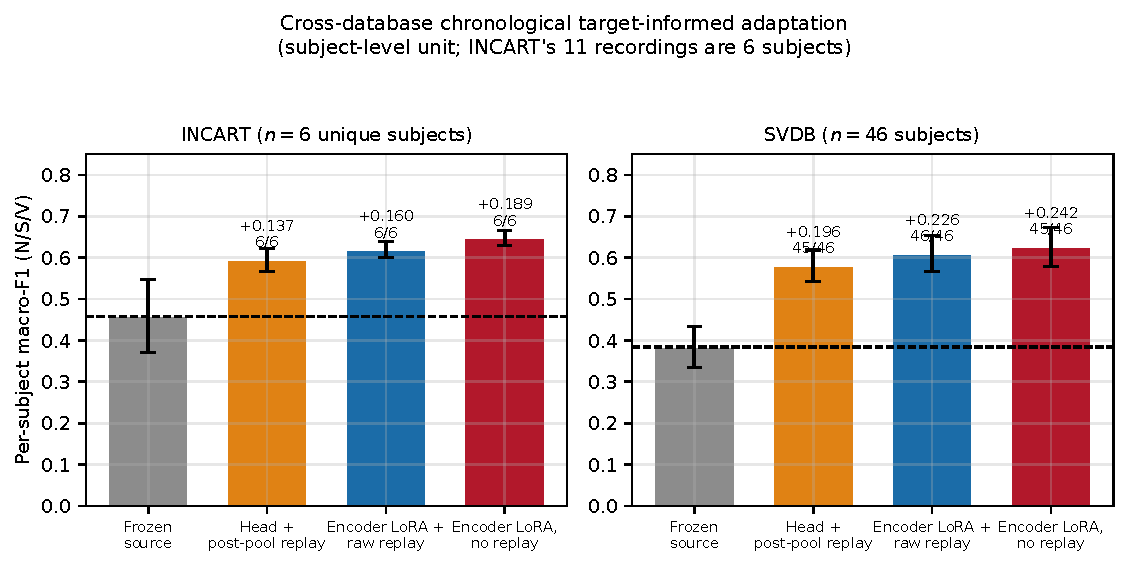
\includegraphics[width=0.9\textwidth]{fig_crossdb_summary.pdf}
\caption{Subject-level cross-database adaptation on INCART and SVDB. INCART
recordings are grouped by the subject identifier in the WFDB header, giving six
unique subjects from 11 recordings; SVDB recordings are one per subject. Every
target-informed method improves per-subject \macrof{} (N/S/V) over the frozen
source (dashed line); annotations give the mean paired gain and the fraction of
subjects improved, and error bars are 95\% bootstrap intervals over subjects.
Encoder LoRA has a higher mean than head-only replay on both external subsets;
no paired direct-comparison interval is reported, so this is not a claim of
statistical superiority. With $n = 6$ the INCART
panel is descriptive rather than inferential.}
\label{fig:crossdb}
\end{figure}

\subsection{RQ7 --- Labeling burden and class coverage}
\label{sec:rq7}

\textbf{Takeaway:} around 100 labelled beats recover roughly 80\% of the
cohort-mean adaptation gain, but \emph{which} labels matter more than how many
--- coverage of the patient's minority class roughly doubles per-patient recovery
(secondary evidence).

Table~\ref{tab:e12_label_curve} and Fig.~\ref{fig:labels} give the label-budget
curve for A4 on the primary cohort under class-aware-oracle and repeated-random
selection at $K \in \{25,50,100,200,500\}$, with patient-bootstrap bands.
\textbf{The class-aware policy is a deliberately non-deployable oracle: it uses
knowledge of which classes later appear in the patient's test segment to choose
which beats to label, and therefore estimates an upper bound on the value of
class coverage rather than a policy a device could execute.} The random policy
is the deployable comparator; where the two differ, the gap is the headroom a
realisable selector would be competing for.
Measured on \emph{cohort means}, the class-aware policy recovers $0.58$ of the
500-label gain at 25 labels, $0.72$ at 50, $0.83$ at 100, and $0.93$ at 200;
random selection recovers $0.54$/$0.64$/$0.78$/$0.89$.

\paragraph{The cohort mean overstates what an individual patient gets.} The
cohort figure is a ratio of mean gains. The quantity a deployment actually cares
about is the per-patient recovery ratio
$R_K = (M_K - M_0)/(M_{500} - M_0)$, and averaging \emph{those} gives a
noticeably weaker picture (Table~\ref{tab:recovery}). Under class-aware
selection the median patient recovers $0.27$ at 25 labels, $0.61$ at 50, $0.67$
at 100, and $0.94$ at 200 --- and \textbf{only $38\%$ of patients individually
reach $R_K \ge 0.8$ at 100 labels}, rising to just $52\%$ at 200. The per-patient
\emph{mean} $R_K$ is unstable at small $K$ (it goes negative) because patients
whose 500-label gain is near zero have a near-zero denominator; we therefore
report the median and the fraction above threshold rather than the mean.

The defensible claim is consequently the narrow one: \emph{around 100 labelled
beats recover roughly 80\% of the cohort-mean adaptation gain under the tested
policies}. It is \textbf{not} true that 100 labels give 80\% of the gain for a
typical individual patient, and we do not claim that 50 labels suffice.

\paragraph{Which labels matter more than how many.} Splitting patients by
whether the adaptation window happened to contain the arrhythmia class that
later appears in the test window is the strongest signal in this experiment. At
100 class-aware labels, patients with that coverage recover $R_K = 0.82$ on
average against $0.41$ for those without --- roughly double. Label \emph{budget}
is therefore the wrong lever to optimize on its own: a small annotated set that
happens to include the patient's minority beats outperforms a larger one that
does not, which argues for coverage-aware annotation prompting rather than
simply asking a clinician for more labels.

\begin{table}[H]
\centering
\small
\caption{E12 label-budget curve for A4 on the 21-record patient-disjoint cohort
(5 seeds). ``Cohort recovery'' is the fraction of the 500-label mean gain over A0
recovered at that budget. Per-patient recovery, which is materially weaker, is in
Table~\ref{tab:recovery}. \emph{Values are seeds mean-averaged within patient;
median unification of this secondary curve is deferred (\texttt{BLOCKERS.md},
ESC-4).}}
\label{tab:e12_label_curve}
\begin{tabular}{lrrrr}
\toprule
Policy & Labels & \macrof{} & 95\% CI & Cohort recovery \\
\midrule
\multirow{5}{*}{Class-aware oracle}
 & 25  & 0.745 & $[0.672,0.818]$ & 0.582 \\
 & 50  & 0.764 & $[0.692,0.835]$ & 0.716 \\
 & 100 & 0.780 & $[0.705,0.853]$ & 0.832 \\
 & 200 & 0.793 & $[0.717,0.867]$ & 0.931 \\
 & 500 & 0.802 & $[0.733,0.873]$ & 1.000 \\
\midrule
\multirow{5}{*}{Repeated random}
 & 25  & 0.740 & $[0.669,0.813]$ & 0.541 \\
 & 50  & 0.754 & $[0.681,0.828]$ & 0.643 \\
 & 100 & 0.773 & $[0.698,0.848]$ & 0.784 \\
 & 200 & 0.787 & $[0.713,0.858]$ & 0.885 \\
 & 500 & 0.802 & $[0.731,0.875]$ & 1.000 \\
\midrule
\multicolumn{5}{l}{\emph{Reference points, full 500 labels, chronological}} \\
 A0 frozen & 500 & 0.666 & $[0.563,0.766]$ & --- \\
 A1 head $+$ max replay & 500 & 0.786 & $[0.712,0.859]$ & --- \\
 A5 LoRA $r{=}2$ & 500 & 0.809 & $[0.734,0.883]$ & --- \\
\bottomrule
\end{tabular}
\end{table}


\begin{table}[H]
\centering
\small
\caption{Label-budget recovery on the 21-record patient-disjoint cohort (5 seeds).
``Cohort'' is the ratio of mean gains, the figure usually quoted; $R_K$ is the
per-patient ratio $(M_K - M_0)/(M_{500} - M_0)$. The per-patient \emph{mean} is
unstable at small $K$ --- patients whose 500-label gain is near zero give a
near-zero denominator --- so the median and the fraction clearing $R_K \ge 0.8$
are the meaningful summaries. The last two columns split patients by whether the
adaptation window contained the arrhythmia class that later appears in the test
window.}
\label{tab:recovery}
\setlength{\tabcolsep}{5pt}
\begin{tabular}{lrrrrrrr}
\toprule
Policy & $K$ & Cohort & Mean $R_K$ & Median $R_K$ & $R_K \ge 0.8$ & $R_K$ covered & $R_K$ not \\
\midrule
\multirow{5}{*}{Class-aware oracle}
 & 25  & 0.582 & $-0.75$ & 0.27 & 19\% & $-0.47$ & $-0.94$ \\
 & 50  & 0.716 & $-0.03$ & 0.61 & 38\% & $0.31$  & $-0.25$ \\
 & 100 & 0.832 & $0.57$  & 0.67 & 38\% & \textbf{0.82} & 0.41 \\
 & 200 & 0.931 & $1.08$  & 0.94 & 52\% & $0.66$  & 1.37 \\
 & 500 & 1.000 & $1.00$  & 1.00 & 100\% & 1.00   & 1.00 \\
\midrule
\multirow{5}{*}{Repeated random}
 & 25  & 0.541 & $-0.56$ & 0.29 & 24\% & $-2.61$ & $-0.36$ \\
 & 50  & 0.643 & $0.02$  & 0.38 & 29\% & $0.17$  & $-0.02$ \\
 & 100 & 0.784 & $0.53$  & 0.66 & 29\% & 0.65    & 0.50 \\
 & 200 & 0.885 & $1.01$  & 0.84 & 52\% & 0.94    & 1.03 \\
 & 500 & 1.000 & $1.00$  & 1.00 & 100\% & 1.00   & 1.00 \\
\bottomrule
\end{tabular}
\end{table}


\begin{figure}[H]
\centering
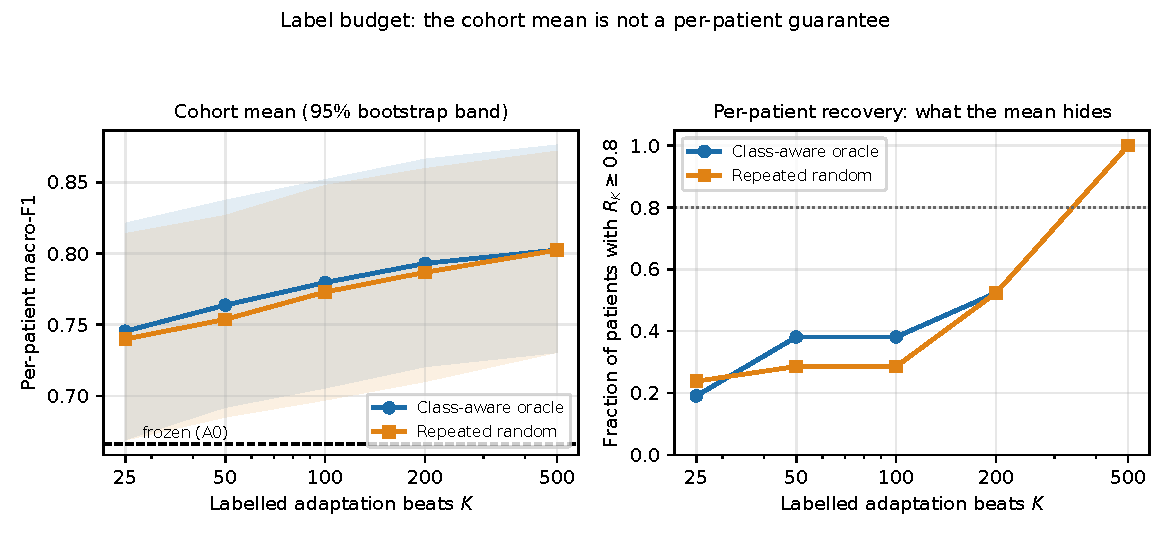
\includegraphics[width=0.78\textwidth]{fig_label_budget_curve.pdf}
\caption{Label budget for A4 on the primary cohort, shown two ways because the
two disagree. \textbf{Left:} cohort-mean \macrof{} with patient-bootstrap 95\%
bands --- the curve usually reported, on which class-aware selection reaches
$\approx 80\%$ of the 500-label gain near 100 labels. \textbf{Right:} the
fraction of \emph{individual} patients whose recovery ratio $R_K$ clears $0.8$
(dotted line). That fraction is $0.38$ at 100 labels and still only $0.52$ at
200, so the left panel must not be read as a per-patient guarantee
(Table~\ref{tab:recovery}).}
\label{fig:labels}
\end{figure}

\subsection{Source-domain change}
\label{sec:srcchange}

\textbf{Takeaway:} tens of raw replay exemplars keep source-domain loss small and
bounded --- encoder arms do not incur larger source-domain loss than head-only
arms despite touching the encoder, and no source class collapses.

Across A1--A5 the source-domain \macrof{} change on the held-out DS1 N/S/V
classes stays within $[-0.048,-0.027]$ (frozen reference $0.946$), and the
five-class change stays within $\pm0.024$. Encoder arms do not incur larger
source-domain loss than head-only arms despite touching the encoder: tens of raw
replay exemplars are enough to anchor it, and no source class collapses. Fig.~\ref{fig:srcchange}
plots per-configuration target gain against source-domain change; the encoder arms
sit in the high-gain, small-source-loss region rather than trading one for the
other.

\begin{figure}[H]
\centering
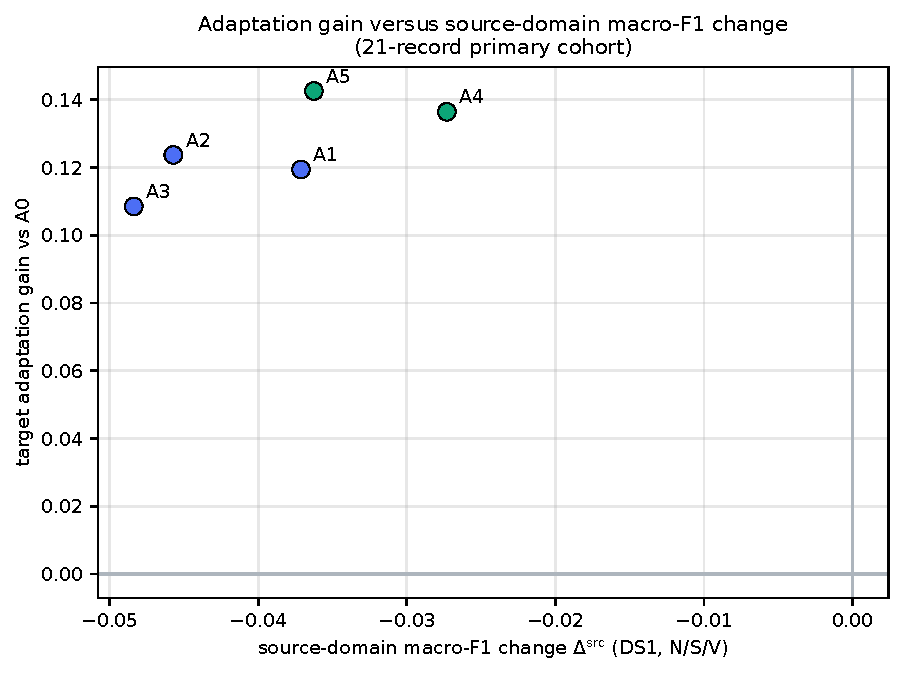
\includegraphics[width=0.80\textwidth]{fig_gain_vs_forgetting.pdf}
\caption{Target patient \macrof{} gain versus the signed source-domain
\macrof{} change $\Delta^{\mathrm{src}}$ (Eq.~\ref{eq:gain_and_srcchange}) for
sweep configurations. $\Delta^{\mathrm{src}}$ is negative when adaptation costs
source performance, so points nearer the top-right retain more of the source
while gaining more on the target. Target gains are not bought with a
proportional source-domain loss; the encoder arms sit near the
stability--plasticity Pareto edge. The axis is labelled source-domain
\macrof{} change throughout; we avoid the word ``forgetting'' because the
quantity measured is a change in DS1 score, not a mechanism.}
\label{fig:srcchange}
\end{figure}

\section{Discussion}
\label{sec:discussion}

\subsection{The replay-point cliff is not an optimization answer}

The cliff measurement is deterministic: only post-pool replay is smaller than
the raw input for this architecture. The primary results change its
interpretation. Compression determines how many exemplars \emph{fit}, but not
how useful the remaining trainable subspace is. Maximum post-pool replay (A1)
fixes the representation and buys volume; raw replay is expensive per item but
leaves budget for attention-level updates. Across all 21 patients, the second
allocation improves more patients (16/21 versus 12/21) and every pooled
minority-class metric, even though it stores an order of magnitude fewer
exemplars. The cliff tells you where you \emph{may} replay; it does not tell you
where you \emph{should}.
\footnote{All primary-cohort figures use the pre-registered locked estimator
(median over seeds within patient, then across patients). Secondary and
sensitivity analyses (E9 ablation, E15 regularization, E16 reserve, E17
split-first, E12 label curve, E13 cross-database) report seeds-mean-averaged
descriptive statistics; those values are flagged where they appear and their
median unification is deferred (\texttt{BLOCKERS.md}, ESC-4).}

\subsection{Why encoder adaptation may help}

The source model has strong V sensitivity but weak S sensitivity. S
identification depends heavily on prematurity and RR context, yet the base
architecture fuses only a two-dimensional RR projection \emph{after} pooling. An
encoder LoRA update can reshape morphology--context interactions upstream of the
pool that a replacement linear head cannot reach. The F-class result is
consistent: post-pool arms plateau near $0.39$ F1 while encoder arms reach
$0.58$--$0.60$. This remains a mechanistic \emph{hypothesis}. RQ5 is the test that
speaks to it most directly, and it is weakly consistent with the hypothesis
rather than confirmatory: starting from sources whose S sensitivity is already
$0.78$--$0.88$ \emph{on their own DS1 test split}, encoder adaptation still
matches head-only replay ($\Delta_{\mathrm{A4-A1}} = +0.0001$ and $+0.0024$).
The adaptation gain persists under two alternative class-reweighted
source-training objectives. This supports robustness to the choice of source
objective, but does not establish robustness to a demonstrably stronger
unseen-patient source model. Those margins are also small and carry no
reported uncertainty, so they do not establish an ordering.

\subsection{What the data support}

Supported by the 21-record patient-disjoint, five-seed primary evidence:
\begin{itemize}[leftmargin=*]
\item patient-specific, target-informed adaptation improves the primary cohort
under the analytical 16\,KiB budget;
\item both encoder-LoRA arms significantly beat the frozen model at patient level
(Holm $p\le0.017$), with large rank-biserial effects and CIs excluding zero ---
these are the \emph{only} two of the six pre-specified comparisons that survive
Holm correction;
\item encoder arms improve more patients and give better pooled S and F
performance than maximum head-only replay, with $\approx 12\times$ fewer
exemplars, though the margin in improved-patient count narrows from four patients
to two once a meaningful-change threshold is applied;
\item the target-side benefit is attributable to encoder plasticity (B4$-$B2,
$p = 0.005$, 16/21 patients); the replay contrast is positive in mean but not
statistically supported (B4$-$B3, $p = 0.473$, median $\approx$ zero), and replay
\emph{volume} shows \textbf{no statistically supported target-side benefit
under the tested selector, replay ratio, optimizer, and patient cohort}
(B1$-$B6, 5 improved / 15 worsened);
\item replay provides substantially better source retention than the tested
zero-byte $B$-factor anchor under the evaluated configuration: at matched bytes,
replay gives $+0.136$ target gain against the anchor's $+0.078$ while losing
about a fifth as much source performance ($-0.027$ versus $-0.136$ \macrof{}),
and the anchor adds nothing once replay is present. Only this one
scale-ambiguous regularizer was tested, so this does not speak to EWC,
distillation, output consistency, or a $\|AB\|_F^2$ penalty
(Section~\ref{sec:reg});
\item about 100 labeled beats recover $\approx 80\%$ of the \emph{cohort-mean}
500-label gain, and whether the adaptation window covers the patient's future
arrhythmia class matters more than the label count (RQ7);
\item the conclusions do not depend on saturating the budget: re-running the
whole grid against a $15{,}360$\,B ceiling, i.e.\ holding back a 1\,KiB firmware
reserve, preserves every significant gain over the frozen model and keeps
encoder adaptation among the top allocations. The \emph{exact arm ordering is
not preserved} --- A1 rises to $0.793$ while A5 falls to $0.792$, putting A4
first --- which is why we read rank-1 as the more robust operating point
(Section~\ref{sec:reserve}).
\end{itemize}

Supported by secondary evidence, on reduced panels or other cohorts:
\begin{itemize}[leftmargin=*]
\item (RQ4) within the measured 12-record Adam panel at ranks 1 and 2, raising
the adaptation-state budget from 8 to 64\,KiB produced no statistically
detectable benefit; 14 of 18 fixed-configuration contrasts met the
pre-specified $\pm 0.05$ equivalence criterion, uncorrected for multiplicity;
\item the adaptation gain survives adaptation from two class-reweighted DS1
sources, of five trained; the encoder-minus-head margins there are nonnegative,
but they are small and carry no reported uncertainty (RQ5);
\item chronological target-informed adaptation transfers to two external
databases at \emph{subject} level, with $+0.14$ to $+0.24$ mean gains on INCART
($6/6$ subjects) and SVDB ($45$--$46/46$); encoder LoRA has the higher mean on
both external subsets, without a paired direct-comparison interval (RQ6).
\end{itemize}

Not supported:
\begin{itemize}[leftmargin=*]
\item direct statistical superiority of A4/A5 over A1 on the primary cohort (the
direct comparisons remain non-significant, and the reweighted-source and
external margins, while consistently positive, are small);
\item any optimizer ranking, or any rank-4/rank-8 statement: SGD is measured only
at 8\,KiB, SGD-with-momentum not at all, and 86 of 140 planned sweep cells are
unrun;
\item \emph{inferential} external validity on INCART: the subject-level gain is
positive with an interval excluding zero, but $n = 6$ subjects supports a
descriptive reading only, and the cohort is a tractability-capped sample of 13 of
75 records rather than a principled selection;
\item RR-architecture and CNN source baselines (three E11 variants still require
new model graphs);
\item any hardware runtime, SRAM, latency, or energy claim;
\item a ``50 labels are sufficient'' claim, or any per-patient reading of the
label curve: at 100 labels only $38\%$ of patients individually reach $80\%$
recovery, so the cohort-mean figure must not be read as a per-patient guarantee.
\end{itemize}

\subsection{Embedded interpretation}

Everything reported here is persistent-state accounting (Appendix~\ref{sec:embedded}
gives the packed record layouts, the memory-category table, and a qualitative
discussion of the unmatched compute paths): trainable weights,
gradients, optimizer moments, replay values, labels, and metadata, packed and
asserted per configuration. It excludes forward and backward activations, stack
and workspace, allocator overhead, and DMA buffers, all of which are peak-SRAM
rather than persistent-state quantities and all of which are implementation- and
toolchain-specific. The 16\,KiB figure is therefore a statement about what a
device must \emph{retain} between adaptation steps, not about what it must have
free at any instant; a hardware study would need to add the runtime terms.

The budget is also accompanied by a firmware implementation reserve. An arm
consuming 16{,}383 of 16{,}384 bytes is not shippable, so we re-generated all
configurations against an effective ceiling of 15{,}360\,B and re-ran every arm
at the reduced replay counts rather than reporting old numbers against new byte
figures. That costs A1 49 exemplars and the encoder arms five each. It changes no
significance conclusion, but it does reshuffle the arm ordering --- A5 is the
arm most sensitive to losing its last few replay samples --- so the reserve
replication is what identifies rank-1 as the safer engineering choice
(Section~\ref{sec:reserve}).

There is one cost of the encoder allocation that the byte budget hides. Raw
replay requires re-forwarding stored beats through the encoder and propagating
gradients through the LoRA training path, whereas post-pool replay enters the
graph after the encoder and bypasses it. Encoder adaptation therefore has
substantially greater compute and energy cost per adaptation step, but
\textbf{this study does not measure or reliably estimate its magnitude} and we
quote no ratio (Appendix~\ref{sec:embedded} explains why the earlier analytical
figure was withdrawn). The arms are matched in bytes and not in compute, which on
a duty-cycled device is an energy difference a deployment study would have to
quantify before choosing between them.

The external result adds a nuance to the frozen-replay story: under strong domain
shift, the no-replay encoder LoRA achieves the \emph{largest} target gain but the
\emph{most} source-domain change. Replay is therefore best understood not as a pure
accuracy lever but as a stability regulator whose value grows with the cost of
source-domain loss.

The regularization comparison sharpens that reading. A parameter-space anchor and
a replay buffer are both stability mechanisms, but they are not
interchangeable: the anchor constrains \emph{how far the weights may move},
whereas replay constrains \emph{what the function must still do}. On a shift that
is a change of patient rather than a change of task, the second constraint is the
useful one, and the measurements bear that out --- at equal persistent bytes,
replay incurs roughly one fifth of the anchor's source-domain loss while also
adapting further. We hold this to its tested scope: \emph{replay provides
substantially better source retention than the tested zero-byte $B$-factor
anchor under the evaluated configuration}. It is one regularizer, in a
scale-ambiguous form, so it does not license the broader claim that a budget
should never be spent on regularization --- restricted EWC, source-logit
distillation, output-consistency regularization, and a $\|AB\|_F^2$ penalty are
all untested here and could behave differently.

\subsection{Backprop memory is not negligible at the KiB scale}

A recent survey of on-device learning in TinyML states the prevailing
assumption directly: ``since all continual learning solutions maintain a replay
buffer of sufficient size to prevent catastrophic forgetting, the memory cost
of backpropagation is unlikely to constitute a bottleneck relative to the buffer
itself'' \cite{pavan2026odlsurvey}. Our two-axis account contradicts this in the
16\,KiB regime. The replay buffer is bounded at 16\,KiB by construction, but the
peak transient working set of the raw-replay encoder arms is $41.3\kib$ even
under block rematerialisation at FP16 (Section~\ref{sec:method},
Appendix~\ref{sec:embedded})---roughly $2.5\times$ the buffer, not a fraction of
it. The assumption holds when the frozen frontend is deep and the buffer is
large; it fails precisely at the KiB scale and pooled-transformer topology
studied here, where a single $8{,}448$-element feed-forward tensor and its
gradient dominate. The correct statement is conditional: backprop memory is
negligible against the buffer only when the trainable subgraph is shallow (as in
post-pool adaptation, whose transient is under $0.1\kib$); for encoder-level
adaptation it is the larger of the two transient charges, and whether it is
affordable depends on how much of it aliases the inference arena the device
already provisions.

There is a corollary for the standard memory-for-compute trade. Block-level
rematerialisation buys the encoder arms a $1.87\times$ peak-transient reduction
($79{,}164 \to 42{,}312\bytes$) at a $1.993\times$ forward-compute multiplier
(\texttt{results/e6\_two\_axis\_accounting.csv}), so at this scale you pay
marginally more in compute than you recover in memory and checkpointing is close
to value-neutral. The reason is structural: the $8{,}448$-element feed-forward
hidden tensor and its gradient dominate the working set so completely that
checkpointing at block granularity cannot escape them, which implies that further
shrinking the encoder-adaptation transient requires finer-grained
rematerialisation or a topology change, not more block checkpointing.

\subsection{Responder structure (exploratory, post-hoc)}

\emph{This subsection is exploratory and post-hoc. It was not pre-registered, it
is hypothesis-generating rather than confirmatory, and it would need its own
pre-registration to be treated as a test. No inferential statistic is reported for
it, and it does not change the pre-registered primary result.}

Looking at where the A4-versus-A1 contrast lives across patients is descriptively
informative. The per-patient median-within A4$-$A1 differences
(\texttt{results/r8\_responder\_exploratory.csv}) split 14 better, 3 exactly
tied, and 4 worse, and range from $-0.033$ to $+0.167$; three patients alone
account for $61\%$ of the total positive mass. In other words the two allocations
look interchangeable for most patients and materially apart for a small
minority. This single observation is consistent, descriptively, with the whole
cluster of otherwise puzzling numbers in Table~\ref{tab:pairwise_tests}: a median
paired difference near zero, a rank-biserial around $0.72$, a mean paired
difference an order of magnitude above the median, and an equivalence test that
fails on its upper bound alone. A natural next question---whether the responding
minority is characterised by higher minority-class support in the adaptation
window---cannot be answered from the released files, which carry no per-record
class-support counts (\texttt{BLOCKERS.md}, ESC-6); we flag it as the follow-up a
dedicated, pre-registered analysis would pursue rather than reporting an untraceable
correlation here.

\subsection{Clinical interpretation}

The method is not an autonomous diagnostic system. It assumes supervised labels
for an early patient segment and evaluates heartbeat classification on curated
research databases. The strong patient heterogeneity---a few records personalize
dramatically, most gain modestly, and a minority regress---is itself a clinical
finding: personalization is unevenly beneficial, and a deployment would need a
per-patient safeguard rather than a blanket ``adaptation always helps''
assumption. The results are algorithmic evidence about memory allocation, not
clinical validation.

\section{Limitations and Remaining Work}
\label{sec:limitations}

We state the current status of each limitation explicitly, including the two that
were previously hard submission gates.

\textbf{The evaluation cohort had to be corrected for a subject leak, and this
matters.} The de Chazal DS1/DS2 split is record-disjoint but not
subject-disjoint: records 201 (DS1) and 202 (DS2) are the same person, per
record 202's own WFDB header. Any result computed on the full 22-record DS2 set
includes one patient the source model was trained on. We audited all 48 records,
found this to be the only such pair, and excluded record 202. The correction is
not cosmetic --- it removed the statistical significance of the A4--A3 contrast
(Holm $p$ $0.047 \to 0.075$), leaving only the two comparisons against the frozen
model surviving correction. Published results on this split that do not exclude
202 are not strictly patient-disjoint and may be optimistically biased by the
same mechanism, and we recommend the check
be run as standard.

\begin{sloppypar}
\textbf{Robustness to source-training objective (RQ5) --- partially addressed.}
Five architecture-identical DS1 source variants (cross-entropy, effective-number
weighting, focal $\gamma\in\{1,2,3\}$) are trained with five seeds and reach
S sensitivity $0.78$--$0.88$ on their own DS1 test split, a figure that motivated
the concern. The adaptation gain persists under two alternative
class-reweighted source-training objectives (Table~\ref{tab:strong_adapt}).
This supports robustness to the choice of source \emph{objective}, but does
\textbf{not} establish robustness to a demonstrably stronger unseen-patient
source model. Three gaps remain.
Adaptation was re-run from two of the five trained
variants, so the robustness claim covers two sources rather than five. The three
RR-placement and CNN variants (RR-conditioned token embedding, RR token before
attention, and a lightweight inter-patient CNN) require new model graphs and
were never trained. The encoder-minus-head margins from the reweighted
checkpoints, while nonnegative, are small and carry no reported uncertainty, so
RQ5 does not independently support an encoder-over-head ordering.
 These
checkpoints are also not \emph{stronger} sources --- on intra-patient DS1 S
sensitivity they are below the cross-entropy baseline --- so RQ5 tests
robustness to the source objective, not adaptation from a stronger start.
\end{sloppypar}

\textbf{Cross-database transfer (RQ6) --- closed at subject level, with a
cohort caveat.} INCART recordings were grouped by the subject identifier in the
WFDB header and the saved cells re-aggregated to one score per subject, so the
external analysis no longer treats repeated recordings from one person as
independent. The gain survives the correction: $+0.160$ \macrof{} for encoder
LoRA over 6 subjects with a bootstrap interval excluding zero and 6/6 subjects
improved, against $+0.226$ over 46 subjects on SVDB. Two limits remain. With
$n = 6$ the INCART result is descriptive rather than inferential, and the INCART
cohort is a tractability-capped convenience sample --- only the first 13 of 75
records were attempted --- so it is not a principled sample of the database. Both
external cohorts now have itemized inclusion and exclusion manifests
(Table~\ref{tab:external_manifest}) in which every configured recording carries
exactly one deterministic disposition. Source-only cross-database generalization
remains weak; it is the target-informed adaptation that is positive.

\textbf{The budget sweep is partial, and named accordingly (RQ4).} Of 140 planned budget $\times$
optimizer $\times$ rank $\times$ replay-location configurations, 49 are measured,
5 are analytically infeasible, and 86 are unrun (Table~\ref{tab:exp_status}). The measured surface is complete
only for Adam at ranks 1--2, and only on a reduced 12-record, 3-seed panel. This
supports only the narrow claim we make---that \emph{within the measured
12-record, three-seed Adam rank-1/rank-2 panel, increasing the budget from 8 to
64\,KiB produced no statistically detectable benefit}, tested by paired contrasts
and TOST equivalence rather than by interval overlap---and supports nothing about
optimizer choice, higher ranks, or budgets outside that panel. Numbers from
this panel are never compared against primary-cohort arms. Following the
completed scope, we describe E10 as an \emph{Adam budget sweep for rank-1 and
rank-2 adaptation}, not as the full optimizer grid it was originally designed
to be.

\textbf{Remaining limitations.} (i)~The primary-cohort direct A4/A5-vs-A1
comparison remains non-significant ($n=21$), so a definitive ``plasticity beats
volume'' claim is not licensed; a larger patient cohort is the most plausible
route to settling it, and the cohort is now one record smaller than the
protocol's nominal size. (ii)~Persistent-state totals are packed and asserted per cell, and the whole grid
was replicated against a 1\,KiB firmware implementation reserve with no change in
conclusions (Section~\ref{sec:reserve}); a byte-exact MCU port would still add
allocator overhead not modeled here. (iii)~Peak SRAM, update latency, update
energy, and Flash write volume are all unmeasured, and no hardware training loop
was executed. \textbf{Training compute, update latency, cycles, and energy are
unmeasured, and no numerical compute ratio is reported}, because the
encoder-LoRA backward cost requires layer-level profiling or a complete
reverse-mode derivation that this study does not provide
(Appendix~\ref{sec:embedded}). (iv)~The regularization family is represented
here by \emph{one inexpensive, memory-matched $B$-factor anchor}
(Section~\ref{sec:reg}), chosen because full-model FP32 EWC costs
$53{,}144$\,B and is infeasible at this budget. Note it anchors the $B$ factor,
not the functional update $BA$. Restricted EWC, distillation from the frozen
model, output-consistency regularization, and functional-delta ($\|AB\|_F^2$)
regularization all remain untested, so this is a comparison against one
convenient member of the family and not against the family. (v)~MIT--BIH is small and old, and Q/paced beats are unsupported in the
primary cohort. (vi)~The reproducibility audit (Table~\ref{tab:audit}) returns 11 PASS, 0 FAIL,
and one WARN: configuration values are fixed in a versioned config file, but no automated
provenance proves the hyperparameters were chosen without access to final test
results. We report the WARN rather than suppressing it; the mitigation is that
hyperparameters are shared across all arms, so any residual selection effect
applies to every arm equally and cannot by itself produce the between-arm
ordering. (vii)~The method assumes supervised labels for an early patient segment
and has had no prospective clinical evaluation.

\textbf{Framing rule.} Under a fixed analytical adaptation-state budget,
patient-specific adaptation of the tiny ECG transformer exhibits a
\emph{replay--plasticity allocation frontier}. Encoder low-rank adaptation with
limited raw replay significantly improves over the frozen model, produces
stronger pooled minority-class performance, and yields more threshold-free
positive patient changes than maximum-volume post-pool replay. However, the
direct average difference from maximum-volume head-only replay is
\textbf{not statistically significant}. The evidence therefore supports co-design
and several competitive operating points rather than a universal winner, and no
sentence in this paper should be read as establishing superiority over A1.

\section{Conclusion}
\label{sec:conclusion}

This software study establishes an algorithmic replay--plasticity trade-off for
memory-constrained, patient-specific adaptation of a tiny ECG transformer, under
a hardware-motivated 16\,KiB persistent-state constraint. The architecture
exhibits a deterministic replay-point cliff---tokens and feed-forward tensors
are several times larger than the raw beat, and only the post-pool
representation is storage-com\-pres\-sive---which makes maximum-volume post-pool
replay the naive budget-optimal design. Over all 21 eligible MIT--BIH DS2
records and five seeds, that naive choice is not established as uniquely optimal:
rank-1 and
rank-2 encoder low-rank adapters with only tens of raw replay samples raise
per-patient \macrof{} from $0.666$ to $0.810$ and $0.811$, improve 16 of 21
patients (versus 12 of 21 for maximum head-only replay), and are both
significant against the frozen model under the pre-registered primary test
(Holm $p\le0.017$) with large effect sizes.
Paired ablations attribute the target gain to encoder plasticity ($p = 0.005$)
but leave replay's direct contribution statistically unsupported ($p = 0.473$),
while replay provides substantially better source retention than the tested
zero-byte $B$-factor anchor under the evaluated configuration; within the
measured 12-record Adam rank-1/rank-2 panel, increasing the adaptation-state
budget from 8 to 64\,KiB produced no statistically detectable benefit, with 14 of
18 fixed-configuration contrasts meeting the pre-specified $\pm 0.05$ equivalence
criterion; and source-domain change stays bounded with no class collapse.

The direct comparison between encoder adaptation and maximum head-only replay is
not statistically significant on the primary cohort, so the honest conclusion is
a \emph{replay--plasticity allocation frontier} rather than ``depth beats
volume.'' Encoder plasticity is more consistent and more replay-efficient at the
same budget, and it carries a higher compute cost; it is not proven strictly
superior to maximum replay, which is simply not established as uniquely optimal.
The frontier holds up under stress, with one caveat we state rather than bury:
the adaptation gain survives when adaptation starts from two class-reweighted
DS1 source checkpoints (of five trained, with S sensitivity $0.78$--$0.88$),
though the encoder-minus-head margins there are small and carry no reported
uncertainty; and the gain reproduces at subject level on two external databases,
where INCART ($6/6$ subjects) and SVDB ($45$--$46/46$) show $+0.14$ to $+0.24$
mean gains, with encoder LoRA again showing the higher mean than head-only
replay. Holding back a
1\,KiB firmware reserve preserves every gain over the frozen model but reshuffles
the arm ordering, which is what makes rank-1 the more robust operating point. What remains is well defined: adaptation from the three
remaining trained source variants, three RR-architecture / CNN variants that were
never trained, the unrun optimizer and higher-rank cells of the budget grid, a
larger external cohort than six INCART subjects, and---for the strong
``plasticity beats volume'' claim---a larger patient cohort that could resolve the
direct comparison, which at $n = 21$ is bounded but inconclusive (neither
superior after correction nor equivalent within the pre-registered
$\delta = 0.02$ margin; minimum detectable effect $\approx 0.01$--$0.04$).
We make no claim of microcontroller deployment; the budget is
analytical persistent state, and peak transient state is reported analytically
under three regimes (Section~\ref{sec:method}) while peak SRAM, latency, and
energy remain for future hardware-in-the-loop work.


\appendix
\section{Experiment Matrix and Reproducibility}
\label{sec:appendix}

\subsection{Experiment ledger}

The package comprises twelve experiments (E6--E17), summarized below with their
status in this manuscript. Cohort and seed count are stated because they differ
between the primary and secondary experiments.

\begingroup
\small
\setlength{\LTcapwidth}{\textwidth}
\begin{longtable}{llp{7.2cm}}
\caption{Experiment status. ``Primary'' denotes the all-DS2 cohort of 21 patient-disjoint records
with five seeds; secondary experiments use reduced panels or other databases and
are never pooled with primary results.}
\label{tab:exp_status}\\
\toprule
ID & Status & Content \\
\midrule
\endfirsthead
\toprule
ID & Status & Content \\
\midrule
\endhead
\bottomrule
\endfoot
E6 & complete & Complete persistent-state accounting for $8/16/32/64$\,KiB, Adam/SGD, INT8 replay; every arm asserted $\le 16{,}384$\,B per cell. \\
E7 & complete (primary) & All-DS2 primary evaluation: 21 patient-disjoint records $\times$ 5 seeds, $\mathrm{gap\_beats}=1$, 630 cells. Record 202 excluded as non-disjoint from DS1 (Section~\ref{sec:cohort}). \\
E8 & complete (primary) & Six pre-specified paired comparisons with Holm correction, patient-bootstrap CIs, and rank-biserial effects. \\
E9 & complete (primary) & Controlled replay-versus-plasticity matrix B0--B7 (B5 infeasible at 16\,KiB) plus fixed-count and fixed-scope controls. \\
E10 & partial (secondary) & \emph{Adam budget sweep for rank-1 and rank-2 adaptation.} Designed as a full budget $\times$ optimizer $\times$ rank grid; executed on a reduced 12-record, 3-seed panel. The subset the paper reports spans 6 configuration families $\times$ 4 budgets $=$ 24 configurations, i.e.\ $24 \times 12 \times 3 = 864$ adaptation cells. Of 140 planned configurations across the broader ledger, 49 are measured, 5 analytically infeasible, 86 unrun (SGD at 8\,KiB only, SGD-with-momentum absent, ranks 4--8 essentially unmeasured). Supports only the budget-saturation claim of Section~\ref{sec:rq4}; no optimizer or higher-rank claim is made. \\
E11 & partial & Five class-reweighted DS1 source checkpoints (CE, effective-number, focal $\gamma1/2/3$) \emph{trained} and measured for source quality with 5 seeds. Adaptation was re-run from \textbf{two} of them (effective-number, focal $\gamma{=}2$), so the robustness claim covers two sources, not five. Three RR-architecture/CNN variants \texttt{not\_implemented\_not\_run}. \\
E12 & complete & Label-budget curve (class-aware and random) with class-coverage and help/harm counts. \\
E13 & complete (subject level) & Cross-database INCART and SVDB: frozen, head-only replay, encoder-LoRA replay, and no-replay encoder-LoRA. The saved cells retain the external record name, so results were re-aggregated to unique subjects (INCART 11 recordings $\rightarrow$ 6 subjects; SVDB one recording per subject) and bootstrapped over subjects. Itemized inclusion/exclusion manifests accompany both databases. \\
E14 & complete & Leakage/reproducibility audit (PASS\,11 / FIXED\,1 / ASSESSED\,1 / WARN\,1 / FAIL\,0), split manifests, source checkpoint hash, config package. \\
E15 & complete (primary) & Memory-matched regularization baseline: rank-1 encoder LoRA with an L2 source anchor $\lambda\sum_m\|B_m\|_F^2$ on the $B$ factor of each attention projection, with (R2) and without (R1) raw replay, 21 records $\times$ 5 seeds $\times$ 2 regularization arms $=$ 210 analysed adaptation cells. The run itself executed 220 cells over the uncorrected 22-record set; the 10 cells belonging to record 202 are excluded from every reported statistic. The anchor costs zero persistent bytes because the frozen base weights are the anchor, so R1 is byte-comparable with B3 and R2 with A4. Penalising $B$ rather than the product $AB$ is scale-ambiguous; reported as a low-cost baseline, not the strongest regularizer. \\
E16 & complete (primary) & Implementation-reserve replication: the full A0--A5 grid re-run against an effective ceiling of $16{,}384 - 1{,}024 = 15{,}360$\,B, which reduces replay counts (A1 $705 \to 656$, A4 $62 \to 57$, A5 $52 \to 47$). 630 cells. Every gain over the frozen model remains significant and encoder adaptation stays among the top allocations; the exact ordering shifts (A5 loses more than A4), making rank-1 the more robust operating point. \\
E17 & complete (sensitivity) & Boundary-leakage sensitivity rerun. The beat store was rebuilt \emph{split-first}: the raw signal is cut at each record's chronological boundary, a $720$-sample ($2$\,s) guard is discarded from each side against a measured $120$-sample filter influence reach, and the two pieces are filtered independently, so no adaptation-side sample can depend on a test-side raw sample. Arms A0, A1, A4, A5 over the same 21 records $\times$ 5 seeds, 420 cells, $497$ adaptation beats per record. Every arm mean moves by $\le 0.007$ \macrof{}; both encoder-versus-frozen contrasts stay significant ($p = 0.0012$) and both encoder-versus-A1 contrasts stay non-significant (Section~\ref{sec:splitfirst}). \\
\end{longtable}
\endgroup

\subsection{Leakage and reproducibility audit}

The audit driver executes twelve automated checks against the released
configuration and the cached beat store, plus two checks added after the original
audit missed them: subject disjointness across the DS1/DS2 split, and filter
support across the chronological boundary. The summary is
\textbf{PASS\,11 / FIXED\,1 / ASSESSED\,1 / WARN\,1 / FAIL\,0}. Both added checks
initially failed. The subject-disjointness failure is \emph{resolved} by excluding
record 202, hence FIXED. The filter-support failure is \emph{characterised rather
than resolved}: the primary pipeline still filters whole records, and E17
(Section~\ref{sec:splitfirst}) shows only that removing the dependency changes no
conclusion --- hence ASSESSED, not FIXED. The warning is reproduced and explained rather than suppressed. We record
the two misses explicitly because an audit that only ever reports PASS is not
evidence of anything.

\begingroup
\small
\setlength{\LTcapwidth}{\textwidth}
\begin{longtable}{lp{3.5cm}p{5.4cm}}
\caption{Audit outcomes and their consequences for the claims in this paper.}
\label{tab:audit}\\
\toprule
Status & Check & Evidence and consequence \\
\midrule
\endfirsthead
\toprule
Status & Check & Evidence and consequence \\
\midrule
\endhead
\bottomrule
\endfoot
PASS & DS1/DS2 record-list disjoint & Record-list intersection empty. \\
\textbf{FIXED} & \textbf{DS1/DS2 \emph{subject} disjoint} & The record lists are disjoint, but records 201 (DS1) and 202 (DS2) are the same subject per 202's WFDB header. All 48 records were audited for this failure mode and 201/202 is the only cross-split pair. Record 202 is now excluded, giving 21 genuinely disjoint evaluation records. This check did not exist in the original audit. \\
PASS & Beat cache coverage & All configured DS1/DS2 records present in the cache; no silent record drops. \\
PASS & Cohort selection is outcome-blind & The primary panel equals the configured DS2 list; later-test arrhythmia burden is not used for inclusion. \\
PASS & Chronological adapt/test split & No record violates ordering; per-record index manifest released. \\
PASS & No window crosses the boundary & The guard beat prevents centred-window overlap; zero overlaps detected. \\
\textbf{ASSESSED} & \textbf{Whole-record filter dependency} & The original audit checked beat-window overlap but not filter support. Baseline-wander median filters and the zero-phase low-pass are applied to the whole record before the split, so adaptation-side samples within $\approx 120$ samples of the boundary depend on test-segment raw samples (no test label, beat, normalization statistic, or model-selection signal is involved). Measured influence reach: $84$ samples at $10^{-3}$ relative tolerance, $120$ at $10^{-5}$. \textbf{The primary pipeline retains this dependency}; E17 (Section~\ref{sec:splitfirst}) removes it and shows that no inferential conclusion changes. This check did not exist in the original audit. \\

PASS & RR normalization uses DS1 only & Computed statistics match the stored source statistics to eight decimals. \\
PASS & No future target statistics & Target RR normalization is called with adaptation-side indices only. \\
PASS & Early stopping is test-blind & Validation slices are drawn from the adaptation$+$replay union. \\
PASS & Per-patient reset & Each cell rebuilds from the frozen backbone; no adapted model carries over. \\
PASS & Source checkpoint pinned & SHA-256 of the DS1 backbone recorded and released. \\
PASS & Seed count & Primary statistics use seeds $\{42,\dots,46\}$. \\
WARN & Hyperparameter selection is final-test independent & Values are fixed in a versioned config file, but no automated provenance proves they were chosen without final-test access. Consequence: a residual selection effect cannot be excluded. Mitigation: the same hyperparameters are used for every arm, so the effect applies uniformly and cannot by itself generate the between-arm ordering. \\
\end{longtable}
\endgroup

\subsection{Runtime environment}

Results were produced with TensorFlow 2.21.0 on a single NVIDIA RTX 3050 (6\,GiB),
seeds $\{42,43,44,45,46\}$, over the \texttt{all\_ds2\_primary} cohort (21 patient-disjoint records).
Derived CSVs, publication figures, and LaTeX tables are regenerated from saved
run reports by a single driver, so each table and figure in this manuscript is
reproducible from the released configurations.

\subsection{Extended ledgers}

Tables~\ref{tab:e11_source_status} (source-baseline ledger) and \ref{tab:e13_crossdb}
(cross-database ledger) are reproduced in Section~\ref{sec:results}. The
label-budget ledger (Table~\ref{tab:e12_label_curve}) additionally reports the
\texttt{secondary\_informative\_panel} single-seed measurements, which are
retained only as secondary evidence and are not used for any headline claim.

\section{Persistent-State Serialization and Compute Scope}
\label{sec:embedded}

This appendix makes every byte in the budget claim reproducible and separates
what the budget covers from what it does not.

\subsection{What the 16\,KiB covers}

\textbf{The 16\,KiB constraint applies to persistent adaptation state, not to
peak training SRAM.} Table~\ref{tab:memcats} lists every memory category and its
status. The included categories are all quantities a device must retain between
adaptation steps; the excluded categories are transient or implementation
specific, and none of them is measured in this work.

\begin{table}[H]
\centering
\small
\caption{Memory categories and their treatment. ``Replication only'' marks the
implementation reserve, which is held back in the reserve replication of
Section~\ref{sec:reserve} but \emph{not} in the primary configuration. No
sentence in this paper claims that total training SRAM is 16\,KiB.}
\label{tab:memcats}
\begin{tabular}{lccl}
\toprule
Memory category & In the 16\,KiB? & Persistent? & Status \\
\midrule
Trainable weights          & yes & yes & analytical \\
Gradients                  & yes & assumption-dependent & analytical \\
Optimizer moments          & yes & yes & analytical \\
Replay values              & yes & yes & analytical \\
Replay labels              & yes & yes & analytical \\
Buffer and quantization metadata & yes & yes & analytical \\
Alignment padding          & yes & yes & analytical \\
Implementation reserve     & replication only & yes & analytical \\
\midrule
Forward activations        & no  & no  & unmeasured \\
Backward activations       & no  & no  & unmeasured \\
Stack and workspace        & no  & no  & unmeasured \\
DMA and allocator overhead & no  & no  & unmeasured \\
Flash write endurance      & no  & --- & unmeasured \\
\bottomrule
\end{tabular}
\end{table}

Gradients are marked assumption-dependent because an implementation that applies
updates immediately per batch need not retain a full gradient vector across
steps. We include them so the accounting is conservative.

\subsection{Packed replay records}

Replay entries are serialized as fixed-stride packed records. With INT8 replay
values, the raw record is

\begin{verbatim}
typedef struct __attribute__((packed)) {
    int8_t  ecg[198];   /* R-peak-centred beat, INT8            */
    int8_t  pre_rr;     /* normalised previous RR interval      */
    int8_t  post_rr;    /* normalised following RR interval     */
    uint8_t label;      /* AAMI class 0..4                      */
    uint8_t valid;      /* slot occupancy flag                  */
    uint8_t class_id;   /* selector bookkeeping                 */
} replay_raw_t;         /* 203 B packed                          */
\end{verbatim}

and the post-pool record is

\begin{verbatim}
typedef struct __attribute__((packed)) {
    int8_t  pooled[16]; /* post-pool embedding, INT8            */
    int8_t  pre_rr;
    int8_t  post_rr;
    uint8_t label;
    uint8_t valid;
    uint8_t class_id;
} replay_postpool_t;    /* 21 B packed                           */
\end{verbatim}

Both structures are all-\texttt{int8}/\texttt{uint8}, so the packed size, the
natural ABI size, and the 1-byte-aligned stride coincide: 203\,B and 21\,B
respectively. Under 4-byte alignment the strides become 204\,B and 24\,B, and
under 8-byte alignment 208\,B and 24\,B; we report the 1-byte figures and
account for the padding explicitly rather than assuming a favorable ABI.

Beyond the per-record fields, each buffer carries fixed metadata: a 4-byte write
index, a 4-byte occupancy count, 16 bytes of reservoir/RNG state, one 4-byte
counter per AAMI class (20\,B), and per-quantized-tensor scale and zero point
(4\,B and 1\,B each). This totals 49\,B for the post-pool buffer, which quantizes
one tensor, and 54\,B for the raw buffer, which quantizes two (the beat and the
RR pair). Table~\ref{tab:arm_definitions} reports the resulting totals.

\subsection{Implementation reserve}

A configuration that consumes 16{,}383 of 16{,}384 bytes is not deployable: it
leaves nothing for a firmware version field, a checksum, or a future field
addition. A deployable rule would hold back a reserve,
\[
B_{\mathrm{used}} \;\le\; B_{\mathrm{budget}} - B_{\mathrm{reserve}},
\]
which at $B_{\mathrm{reserve}} = 1024$\,B lowers the effective ceiling to
15{,}360\,B.

We are explicit about how this relates to the results, because the two are easy
to conflate. \textbf{The primary analysis does \emph{not} apply a reserve.} Its
configurations are generated against the full 16{,}384\,B ceiling, because that
is what the pre-specified analysis plan fixed, and changing the byte rule after
the fact would forfeit the pre-specification. The reserve is instead reported as
a \emph{separate replication} (Section~\ref{sec:reserve},
Table~\ref{tab:reserve}): the entire A0--A5 grid re-run at the 15{,}360\,B
ceiling with regenerated replay counts, which preserves every significant gain
over the frozen model but \emph{not} the exact arm ordering --- A1 rises to
$0.793$ and A5 falls to $0.792$, so A4 leads under the reserve where A5 leads
without it. Table~\ref{tab:arm_definitions} lists both count sets side
by side so no arm's performance is ever quoted against a byte figure it was not
measured under. A deployment should use the reserved counts; the primary table
documents the pre-specified configuration.

\subsection{Compute is not matched across arms}

The arms are matched on persistent bytes but \emph{not} on compute, and the
direction of the gap is unambiguous even though this paper does not quantify it.
Raw replay requires re-forwarding stored beats through the encoder and
propagating gradients through the LoRA training path, whereas post-pool replay
enters the graph after the encoder and bypasses it entirely. Encoder adaptation
therefore carries a substantially greater compute and energy cost per adaptation
step than head-only or post-pool replay.

\textbf{We do not report a numeric ratio.} An earlier version of this appendix
gave analytical MAC totals and a fixed multiplier, charging backward cost as a
multiple of the forward cost of the trainable path only. That convention is
defensible for the head and post-pool arms, whose trainable parameters sit after
the frozen encoder, but it is not a safe basis for a headline number in the
encoder-LoRA arms: reverse-mode differentiation must propagate activation
gradients \emph{through} frozen operations to reach LoRA factors inserted inside
the encoder, so a backward pass cannot be priced from the trainable parameter
count alone. Rather than publish a ratio whose derivation we cannot fully stand
behind, we state the qualitative asymmetry and leave the magnitude to a
measured study --- a layer-by-layer forward and backward derivation, or a
profiler trace on the target runtime --- in the journal version.

This matters for a deployment decision and not for the allocation result. The
memory-allocation contribution of this paper is an accounting of persistent
\emph{bytes}, and every comparison in it is byte-matched by construction; none
of the conclusions depends on the compute figures withdrawn here. A reader
choosing between these arms on a duty-cycled device should nevertheless treat
encoder adaptation as the more expensive option and measure it before
committing.


\section*{Declarations}
\addcontentsline{toc}{section}{Declarations}

\paragraph{Corresponding author.} Subhajit Roy,
\texttt{subhajitroy005@gmail.com}.

\paragraph{Ethics.} This study used publicly available, de-identified
physiological databases distributed through PhysioNet
\cite{goldberger2000physiobank,moody2001impact,greenwald1990svdb} and did not
involve new human-subject recruitment or intervention. No ethical approval was
required.

\paragraph{Data availability.} All data are public: the MIT--BIH Arrhythmia
Database, the St.\ Petersburg INCART 12-lead Arrhythmia Database, and the
MIT--BIH Supraventricular Arrhythmia Database, all obtainable from PhysioNet.
The DS1/DS2 record partitions, the external inclusion and exclusion manifests,
the INCART record-to-subject map, and every derived summary CSV behind the
tables and figures are released with the code at the repository below.

\paragraph{Code availability.} The adaptation framework, the constrained
configuration generator, the memory-accounting module, the statistical
pipeline, and the figure and table generators are released together with the
run configurations, the random seeds, and the environment specification needed
to reproduce every number in this paper. Every published value is regenerated
from released artifacts by a single driver
(\texttt{scripts/reproduce\_paper.py}); no result is transcribed by hand.

\vspace{0.3em}
\noindent
\begin{tabular}{@{}ll@{}}
Repository & \url{https://github.com/subhajitroy005/BudgetCL-ECG} \\
Software release & \texttt{v1.0.0-arxiv} (annotated, immutable tag) \\
\end{tabular}

\vspace{0.3em}
\noindent
The annotated, immutable Git tag \texttt{v1.0.0-arxiv} is the primary software
identifier and resolves unambiguously to the exact release commit. The release
manifest records artifact checksums, configuration identifiers, environment
information, and the release tag.

\noindent
The DS1 source checkpoint these results adapt from is pinned by

\vspace{0.2em}
\noindent\hspace*{\fill}%
\texttt{SHA-256 a6d4eff14caa4404eb57dc5e\-b9ecfcb9e9d3f1a1bf907d6d147fb5611eb79fce}%
\hspace*{\fill}
\vspace{0.2em}

\noindent
so a reproduction can verify it is starting from the same model. Raw PhysioNet
recordings are not redistributed; the repository provides download scripts and
itemized inclusion/exclusion manifests instead.

\paragraph{Funding.} This work received no external funding.

\paragraph{Competing interests.} The author declares no competing interests.

\paragraph{Author contributions.} S.R.\ conceived the study, implemented the
framework and experiments, performed the analysis, and wrote the manuscript.

\paragraph{Use of AI assistance.} An AI coding assistant was used for software
implementation, for generating analysis and figure scripts, and for editorial
assistance during manuscript preparation. All experimental design decisions,
all claims, and all interpretations are the author's; every reported number is
produced by the released code from saved run artifacts, and the author has
verified the correspondence between the manuscript and those artifacts.


\begin{thebibliography}{99}

\bibitem{busia2025tiny}
P. Busia, M. A. Scrugli, V. J.-B. Jung, L. Benini, and P. Meloni,
``A Tiny Transformer for Low-Power Arrhythmia Classification on
Microcontrollers,'' \emph{IEEE Transactions on Biomedical Circuits and
Systems}, vol. 19, no. 1, pp. 142--152, 2025,
doi: 10.1109/TBCAS.2024.3401858.

\bibitem{moody2001impact}
G. B. Moody and R. G. Mark,
``The Impact of the MIT-BIH Arrhythmia Database,''
\emph{IEEE Engineering in Medicine and Biology Magazine},
vol. 20, no. 3, pp. 45--50, 2001,
doi: 10.1109/51.932724.

\bibitem{goldberger2000physiobank}
A. L. Goldberger \emph{et al.},
``PhysioBank, PhysioToolkit, and PhysioNet: Components of a New Research
Resource for Complex Physiologic Signals,''
\emph{Circulation}, vol. 101, no. 23, pp. e215--e220, 2000,
doi: 10.1161/01.CIR.101.23.e215.

\bibitem{dechazal2004automatic}
P. de Chazal, M. O'Dwyer, and R. B. Reilly,
``Automatic Classification of Heartbeats Using ECG Morphology and Heartbeat
Interval Features,''
\emph{IEEE Transactions on Biomedical Engineering},
vol. 51, no. 7, pp. 1196--1206, 2004,
doi: 10.1109/TBME.2004.827359.

\bibitem{pellegrini2020latent}
L. Pellegrini, G. Graffieti, V. Lomonaco, and D. Maltoni,
``Latent Replay for Real-Time Continual Learning,''
in \emph{Proc. IEEE/RSJ International Conference on Intelligent Robots and
Systems}, 2020, pp. 10203--10209,
doi: 10.1109/IROS45743.2020.9341460.

\bibitem{ravaglia2021tinyml}
L. Ravaglia, M. Rusci, D. Nadalini, A. Capotondi, F. Conti, and L. Benini,
``A TinyML Platform for On-Device Continual Learning With Quantized Latent
Replays,''
\emph{IEEE Journal on Emerging and Selected Topics in Circuits and Systems},
vol. 11, no. 4, pp. 789--802, 2021,
doi: 10.1109/JETCAS.2021.3121554.

\bibitem{kirkpatrick2017overcoming}
J. Kirkpatrick \emph{et al.},
``Overcoming Catastrophic Forgetting in Neural Networks,''
\emph{Proceedings of the National Academy of Sciences},
vol. 114, no. 13, pp. 3521--3526, 2017,
doi: 10.1073/pnas.1611835114.

\bibitem{hu2022lora}
E. J. Hu, Y. Shen, P. Wallis, Z. Allen-Zhu, Y. Li, S. Wang, L. Wang,
and W. Chen,
``LoRA: Low-Rank Adaptation of Large Language Models,''
in \emph{International Conference on Learning Representations}, 2022.

\bibitem{douillard2022dytox}
A. Douillard, A. Ram\'e, G. Couairon, and M. Cord,
``DyTox: Transformers for Continual Learning With Dynamic Token Expansion,''
in \emph{Proc. IEEE/CVF Conference on Computer Vision and Pattern
Recognition}, 2022, pp. 9285--9295.

\bibitem{lin2022ondevice}
J. Lin, L. Zhu, W.-M. Chen, W.-C. Wang, C. Gan, and S. Han,
``On-Device Training Under 256KB Memory,''
in \emph{Advances in Neural Information Processing Systems},
vol. 35, 2022, pp. 22941--22954.

\bibitem{rebuffi2017icarl}
S.-A. Rebuffi, A. Kolesnikov, G. Sperl, and C. H. Lampert,
``iCaRL: Incremental Classifier and Representation Learning,''
in \emph{Proc. IEEE Conference on Computer Vision and Pattern Recognition},
2017, pp. 2001--2010.

\bibitem{tiwari2022gcr}
R. Tiwari, K. Killamsetty, R. Iyer, and P. Shenoy,
``GCR: Gradient Coreset Based Replay Buffer Selection for Continual
Learning,''
in \emph{Proc. IEEE/CVF Conference on Computer Vision and Pattern
Recognition}, 2022, pp. 99--108.

\bibitem{borsos2020coresets}
Z. Borsos, M. Mutn\'y, M. Tagliasacchi, and A. Krause,
``Coresets via Bilevel Optimization for Continual Learning and Streaming,''
in \emph{Advances in Neural Information Processing Systems},
vol. 33, 2020, pp. 14879--14890.


\bibitem{hu1997patient}
Y. H. Hu, S. Palreddy, and W. J. Tompkins,
``A Patient-Adaptable ECG Beat Classifier Using a Mixture of Experts
Approach,''
\emph{IEEE Transactions on Biomedical Engineering},
vol. 44, no. 9, pp. 891--900, 1997,
doi: 10.1109/10.623058.

\bibitem{kiranyaz2016realtime}
S. Kiranyaz, T. Ince, and M. Gabbouj,
``Real-Time Patient-Specific ECG Classification by 1-D Convolutional Neural
Networks,''
\emph{IEEE Transactions on Biomedical Engineering},
vol. 63, no. 3, pp. 664--675, 2016,
doi: 10.1109/TBME.2015.2468589.

\bibitem{llamedo2011heartbeat}
M. Llamedo and J. P. Mart\'inez,
``Heartbeat Classification Using Feature Selection Driven by Database
Generalization Criteria,''
\emph{IEEE Transactions on Biomedical Engineering},
vol. 58, no. 3, pp. 616--625, 2011,
doi: 10.1109/TBME.2010.2068048.

\bibitem{mar2011optimization}
T. Mar, S. Zaunseder, J. P. Mart\'inez, M. Llamedo, and R. Poll,
``Optimization of ECG Classification by Means of Feature Selection,''
\emph{IEEE Transactions on Biomedical Engineering},
vol. 58, no. 8, pp. 2168--2177, 2011,
doi: 10.1109/TBME.2011.2113395.

\bibitem{hannun2019cardiologist}
A. Y. Hannun, P. Rajpurkar, M. Haghpanahi, G. H. Tison, C. Bourn,
M. P. Turakhia, and A. Y. Ng,
``Cardiologist-Level Arrhythmia Detection and Classification in Ambulatory
Electrocardiograms Using a Deep Neural Network,''
\emph{Nature Medicine}, vol. 25, no. 1, pp. 65--69, 2019,
doi: 10.1038/s41591-018-0268-3.

\bibitem{greenwald1990svdb}
S. D. Greenwald,
``Improved Detection and Classification of Arrhythmias in Noise-Corrupted
Electrocardiograms Using Contextual Information,''
Ph.D. dissertation, Harvard--MIT Division of Health Sciences and Technology,
Massachusetts Institute of Technology, Cambridge, MA, USA, 1990.

\bibitem{ansi2012aami}
Association for the Advancement of Medical Instrumentation,
\emph{Testing and Reporting Performance Results of Cardiac Rhythm and
ST-Segment Measurement Algorithms}, ANSI/AAMI EC57:2012, 2012.

\bibitem{houlsby2019adapters}
N. Houlsby, A. Giurgiu, S. Jastrzebski, B. Morrone, Q. de Laroussilhe,
A. Gesmundo, M. Attariyan, and S. Gelly,
``Parameter-Efficient Transfer Learning for NLP,''
in \emph{Proc. International Conference on Machine Learning},
2019, pp. 2790--2799.

\bibitem{cai2020tinytl}
H. Cai, C. Gan, L. Zhu, and S. Han,
``TinyTL: Reduce Memory, Not Parameters for Efficient On-Device Learning,''
in \emph{Advances in Neural Information Processing Systems},
vol. 33, 2020, pp. 11285--11297.

\bibitem{wang2021tent}
D. Wang, E. Shelhamer, S. Liu, B. Olshausen, and T. Darrell,
``Tent: Fully Test-Time Adaptation by Entropy Minimization,''
in \emph{International Conference on Learning Representations}, 2021.

\bibitem{liang2020shot}
J. Liang, D. Hu, and J. Feng,
``Do We Really Need to Access the Source Data? Source Hypothesis Transfer for
Unsupervised Domain Adaptation,''
in \emph{Proc. International Conference on Machine Learning},
2020, pp. 6028--6039.

\bibitem{lin2017focal}
T.-Y. Lin, P. Goyal, R. Girshick, K. He, and P. Doll\'ar,
``Focal Loss for Dense Object Detection,''
in \emph{Proc. IEEE International Conference on Computer Vision},
2017, pp. 2980--2988.

\bibitem{cui2019classbalanced}
Y. Cui, M. Jia, T.-Y. Lin, Y. Song, and S. Belongie,
``Class-Balanced Loss Based on Effective Number of Samples,''
in \emph{Proc. IEEE/CVF Conference on Computer Vision and Pattern
Recognition}, 2019, pp. 9268--9277.

\bibitem{vaswani2017attention}
A. Vaswani, N. Shazeer, N. Parmar, J. Uszkoreit, L. Jones, A. N. Gomez,
{\L}. Kaiser, and I. Polosukhin,
``Attention Is All You Need,''
in \emph{Advances in Neural Information Processing Systems},
vol. 30, 2017, pp. 5998--6008.

\bibitem{li2018lwf}
Z. Li and D. Hoiem,
``Learning Without Forgetting,''
\emph{IEEE Transactions on Pattern Analysis and Machine Intelligence},
vol. 40, no. 12, pp. 2935--2947, 2018,
doi: 10.1109/TPAMI.2017.2773081.

\bibitem{chaudhry2019tiny}
A. Chaudhry, M. Rohrbach, M. Elhoseiny, T. Ajanthan, P. K. Dokania,
P. H. S. Torr, and M. Ranzato,
``On Tiny Episodic Memories in Continual Learning,''
\emph{arXiv:1902.10486}, 2019.

\bibitem{lopezpaz2017gem}
D. Lopez-Paz and M. Ranzato,
``Gradient Episodic Memory for Continual Learning,''
in \emph{Advances in Neural Information Processing Systems},
vol. 30, 2017, pp. 6467--6476.

\bibitem{zenke2017si}
F. Zenke, B. Poole, and S. Ganguli,
``Continual Learning Through Synaptic Intelligence,''
in \emph{Proc. International Conference on Machine Learning},
2017, pp. 3987--3995.

\bibitem{banbury2021mlperftiny}
C. Banbury \emph{et al.},
``MLPerf Tiny Benchmark,''
in \emph{Proc. Neural Information Processing Systems Datasets and Benchmarks
Track}, 2021.

\bibitem{david2021tflitemicro}
R. David \emph{et al.},
``TensorFlow Lite Micro: Embedded Machine Learning for TinyML Systems,''
in \emph{Proc. Machine Learning and Systems (MLSys)}, vol. 3, 2021,
pp. 800--811.


\bibitem{ruib2024tinyml}
M. R\"ub, P. Tuchel, A. Sikora, and D. Mueller-Gritschneder,
``A Continual and Incremental Learning Approach for TinyML On-Device Training
Using Dataset Distillation and Model Size Adaption,''
\emph{arXiv:2409.07114}, 2024.

\bibitem{replay2025survey}
H.-S. Park, H.-C. Chu, M.-K. Sung, C. Kim, J. Lee, D.-W. Kim, and J. Lee,
``Survey on Replay-Based Continual Learning and Empirical Validation on
Feasibility in Diverse Edge Devices Using a Representative Method,''
\emph{Mathematics}, vol. 13, no. 14, art. 2257, 2025,
doi: 10.3390/math13142257.

\bibitem{ecgfoundation2024survey}
Y. Han, V. Murino, X. Liu, X. Zhang, and C. Ding,
``A Systematic Review on Foundation Models for Electrocardiogram Analysis:
Initial Strides and Expansive Horizons,''
\emph{arXiv:2410.19877}, 2024.

\bibitem{zhang2026amrecl}
P. Zhang, J. Yang, Y. Yao, X. Ruan, Y. Chen, X. Wang, and Y. Chen,
``Adaptive Memory Replay for Plasticity-Aware Edge Continual Learning,''
\emph{Expert Systems with Applications}, in press, available online 2026;
assigned to vol. 331, art. 133393 (issue dated 15 December 2026),
doi: 10.1016/j.eswa.2026.133393.

\bibitem{ravaglia2020memlatacc}
L. Ravaglia, M. Rusci, A. Capotondi, F. Conti, L. Pellegrini, V. Lomonaco,
D. Maltoni, and L. Benini,
``Memory-Latency-Accuracy Trade-Offs for Continual Learning on a RISC-V
Extreme-Edge Node,'' in \emph{2020 IEEE Workshop on Signal Processing Systems
(SiPS)}, 2020, pp. 1--6, doi: 10.1109/SIPS50750.2020.9195220.

\bibitem{mitdb202note}
PhysioNet, ``MIT--BIH Arrhythmia Database, record 202 header (\texttt{202.hea}),''
MIT--BIH Arrhythmia Database v1.0.0, PhysioNet, 2005.
[Online]. Available: \url{https://physionet.org/content/mitdb/1.0.0/202.hea}

\bibitem{zheng2026ewclora}
Y. Zheng, Y. Zhang, J. van de Weijer, G. M. van de Ven, S. Du, X. Zhang, and
Z. Tian, ``Revisiting Weight Regularization for Low-Rank Continual Learning,''
in \emph{International Conference on Learning Representations (ICLR)}, 2026.
[Online]. Available: \url{https://arxiv.org/abs/2602.17559}

\bibitem{shahbazinia2025epismart}
A. Shahbazinia, J. Dan, J. A. Miranda, G. Ansaloni, and D. Atienza,
``Personalization on a Budget: Minimally-Labeled Continual Learning for
Resource-Efficient Seizure Detection,'' 2025.
[Online]. Available: \url{https://arxiv.org/abs/2509.13974}

\bibitem{bassobert2025binaryreplay}
Y. Basso-Bert, A. Molnos, R. Lemaire, W. Guicquero, and A. Dupret,
``Towards Experience Replay for Class-Incremental Learning in Fully-Binary
Networks,'' 2025.
[Online]. Available: \url{https://arxiv.org/abs/2503.07107}

\bibitem{barusco2026vadedge}
M. Barusco, F. Borsatti, D. Petrovic, D. Dalle Pezze, and G. A. Susto,
``Continual Visual Anomaly Detection on the Edge: Benchmark and Efficient
Solutions,'' 2026.
[Online]. Available: \url{https://arxiv.org/abs/2604.06435}

\bibitem{pavan2026odlsurvey}
M. Pavan, L. Pezzarossa, F. Pittorino, M. Roveri, and X. Fafoutis,
``What Changes After Deployment? A Survey on On-Device Learning in TinyML,''
2026. [Online]. Available: \url{https://arxiv.org/abs/2605.31226}

\end{thebibliography}


\end{document}
